%%%%%%%%%%%%%%%%%%%%%%%%%%%%%%%%%%%%%%%%%%%%%%%%%%%%%%%
%
%                                                       Example IS Template
%
% \documentclass{woosterthesis} must be at the beginning of every IS. Options are the same as
% for the report class with some additional options, abstractonly, blacklinks, code, kaukecopyright, palatino, picins,
% maple, index, verbatim, dropcaps, euler, gauss, alltt,  woolshort, colophon, woosterchicago, and
% achemso. The kaukecopyright option will put the arch symbol with the word mark on the
% copyright page. The woosterthesis class is based on the report class. One thing to note is that
% the ``%'' symbol comments out all characters that follow it on the line.
%
%%%%%%%%%%%%%%%%%%%%%%%%%%%%%%%%%%%%%%%%%%%%%%%%%%%%%%%

%%%%%%%%%%%%%%%%%%%%%%%%%%%%%%%%%%%%%%%%%%%%%%%%%%%%%%%
%
% Checked on 8/26/22 and compiles with no fatal errors. Users must have the latest version of the TeXLive software and
% have installed all available packages from CTAN to ensure this thesis class compiles with no fatal errors. Also, you must
% run pdfLaTex, Biber, MakeIndex, padfLaTeX, pdfLaTeX to get all the numbering and references resolved. This is the
% first year the template uses Biber for references.
%
%%%%%%%%%%%%%%%%%%%%%%%%%%%%%%%%%%%%%%%%%%%%%%%%%%%%%%%

%%%%%%%%%%%%%%%%%%%%%%%%%%%%%%%%%%%%%%%%%%%%%%%%%%%%%%%
% use this declaration for a draft  version of your IS
\documentclass[10pt,palatino,code,picins,tikz,kaukecopyright,openright,lshortwooster,dropcaps,verbatim,index,euler]{woosterthesis}
% \documentclass[10pt,code,picins,kaukecopyright,openright,woolshort,dropcaps,verbatim,euler,index,colophon,twoside]{woosterthesis}
% note that you can specify the chicago option to use Chicago citation style and acs to use the American Chemical Society citation format
%
%%%%%%%%%%%%%%%%%%%%%%%%%%%%%%%%%%%%%%%%%%%%%%%%%%%%%%%
%
% use this declaration for the print version of your IS
%\documentclass[12pt,code,palatino,picins,blacklinks,kaukecopyright,openright,twoside]{woosterthesis} % probably what most students would use
%
%%%%%%%%%%%%%%%%%%%%%%%%%%%%%%%%%%%%%%%%%%%%%%%%%%%%%%%
%
% use this declaration for the PDF version of your IS
% \documentclass[12pt,code,palatino,picins,kaukecopyright,openright,twoside]{woosterthesis}
%
%%%%%%%%%%%%%%%%%%%%%%%%%%%%%%%%%%%%%%%%%%%%%%%%%%%%%%%

%%%%%%%%%%%%%%%%%%%%%%%%%%%%%%%%%%%%%%%%%%%%%%%%%%%%%%%
%
%                                                       Load Packages
%
%   To load packages in addition to the ones that are loaded by default, please place your
%   usepackage commands in the packages.tex file in the styles folder.
%
%%%%%%%%%%%%%%%%%%%%%%%%%%%%%%%%%%%%%%%%%%%%%%%%%%%%%%%

%%%%%%%%%%%%%%%%%%%%%%%%%%%%%%%%%%%%%%%%%%%%%%%%%%%%%%%%%%%%%%%%%%%%%%%%%%%%%%%%%%%%%%%%%%%%%%
%
%                                                       Packages
%
% Do not add any other packages without consulting with Dr. Breitenbucher as they may break the functionality of the class.
%
%%%%%%%%%%%%%%%%%%%%%%%%%%%%%%%%%%%%%%%%%%%%%%%%%%%%%%%%%%%%%%%%%%%%%%%%%%%%%%%%%%%%%%%%%%%%%%

\ifxetex%
	\defaultfontfeatures{Mapping=tex-text,Ligatures=TeX}%
		\setmainfont[Numbers=OldStyle,BoldFont={* Semibold}]{Adobe Garamond Pro}% select the body font other choices would be Baskerville, Optima Regular, Didot, Georgia, Cochin
                      \setmathrm{Adobe Garamond Pro}
                      \setmathfont[Digits,Latin]{Adobe Garamond Pro}
		\setsansfont[Scale=.87,Fractions=On,Numbers=Lining]{Myriad Pro}% select the sans serif font other choices would be Skia, Arial, Helvetica, Helvetica Neue
%		\setmonofont[Scale=.88,Fractions=On]{Prestige Elite Std Bold}% set the mono font other choices would be Courier, Monaco, American Typewriter
	           \setmonofont[Scale=.9]{Courier Std}%
%	    \setromanfont[Fractions=On,Numbers=OldStyle, BoldFont={Warnock Pro Semibold}]{Warnock Pro}%
%	    \setsansfont[Scale=.95,Fractions=On,Numbers=Lining]{Myriad Pro}%
%	    \setmonofont[Scale=.91,Fractions=On]{Courier Std Medium}%
%	    \setmonofont[Scale=.88,Fractions=On]{American Typewriter}%
%		\setmonofont[Scale=.94,Fractions=On]{Prestige Elite Std Bold}
%    		\setromanfont[Fractions=On,Numbers=OldStyle]{Minion Pro}
 %    	\setsansfont[Scale=.9,Fractions=On,Numbers=Lining]{Myriad Pro}
%     	\setmonofont[Scale=.93,Fractions=On]{Courier Std Medium}
%     	\setromanfont[Fractions=On,Numbers=OldStyle]{Minion Pro}
%     	\setsansfont[Scale=.85,Fractions=On,Numbers=Lining]{News Gothic Std}
%    		\setmonofont[Scale=.93,Fractions=On]{Prestige Elite Std}
%		\setromanfont[Fractions=On,Numbers=OldStyle]{Minion Pro}
%		\setsansfont[Scale=.9,Fractions=On,Numbers=Lining]{Bell Gothic Std Bold}
%		\setmonofont[Scale=.95,Fractions=On]{Prestige Elite Std Bold}
\fi

%%%%%%%%%%%%%%%%%%%%%%%%%%%%%%%%%%%%%%%%%%%%%%%%%%%%%%%
%
%                                                       Load Personal commands
%                                                                    
%  There will be certain commands that you use frequently in the thesis. You can give these
%  commands new names which are easier for you to remember. You can also combine several
%  commands into a new command of your own. See The LaTeX Companion or Guide to LaTeX
%  for examples on defining your own commands. These are commands that I defined to cut
%  down on typing. You can enter your commands in the personal.tex file in the styles folder.
%
%%%%%%%%%%%%%%%%%%%%%%%%%%%%%%%%%%%%%%%%%%%%%%%%%%%%%%%

%%%%%%%%%%%%%%%%%%%%%%%%%%%%%%%%%%%%%%%%%%%%%%%%%%%%%%%%%%%%%%%%%%%%%%%%%%%%%%%%%%%%%%%%%%%%%%
%
%                                                       Personal Commands
%                                                                    
% There will be certain commands that you use frequently in the thesis. You can give these
% commands new names which are easier for you to remember. You can also combine several
% commands into a new command of your own. See The LaTeX Companion or Guide to LaTeX for
% examples on defining your own commands. These are commands that I defined to cut down on typing.
%
%%%%%%%%%%%%%%%%%%%%%%%%%%%%%%%%%%%%%%%%%%%%%%%%%%%%%%%%%%%%%%%%%%%%%%%%%%%%%%%%%%%%%%%%%%%%%%

\newcommand{\fl}{\ell}
\newcommand{\lt}{\LaTeX\ }
\newcommand{\msw}{Word\texttrademark\ }
\newcommand{\xt}{\ifthenelse{\boolean{xetex}}{\XeTeX\ }{XeTeX} }
%\newcommand{\Cl}{\ensuremath{\textup{C}_\fl}}
%\newcommand{\bCl}{C$_{\ell}$}
%\newcommand{\Al}{\ensuremath{\textup{A}_\fl}}
%\newcommand{\msum}{{(m_1+\cdots+m_\ell)}}
%\newcommand{\Nsum}{{(N_1+\cdots+N_\ell)}}
%\newcommand{\ysum}{{(y_1+\cdots+y_\ell)}}
%\newcommand{\Nsub}{{N_1+\cdots+N_\ell}}
%\newcommand{\ysub}{{y_1+\cdots+y_\ell}}
%\newcommand{\xsub}{{x_1+\cdots+x_\ell}}
%\newcommand{\ysqsum}{{y_1^2+\cdots +y_{\fl}^2}}
%\newcommand{\msqsum}{{m_1^2+\cdots +m_{\fl}^2}}
%\newcommand{\ratio}{\left(\frac{\beta}{\alpha}\right)}
%\newcommand{\LT}{\ensuremath{\LaTeX{}}}

%%%%%%%%%%%%%%%%%%%%%%%%%%%%%%%%%%%%%%%%%%%%%%%%%%%%%%%%%%%%%%%%%%%%%%%%%%%%%%%%%%%%%%%%%%%%%%
% These commands have one argument and are entered as \commandname{argument}.
%%%%%%%%%%%%%%%%%%%%%%%%%%%%%%%%%%%%%%%%%%%%%%%%%%%%%%%%%%%%%%%%%%%%%%%%%%%%%%%%%%%%%%%%%%%%%%

%\newcommand{\bd}[1]{\textbf{#1}}
\newcommand{\mbd}[1]{{\mathbf{#1}}}
%\newcommand{\abs}[1]{\vert{#1}\vert}
\newcommand{\bvec}[1]{{\mbd{#1}}}
%\newcommand{\lvec}[1]{\abs{\bvec{#1}}}
%\newcommand{\nesmallprod}[1]{\prod_{\substack{#1=1\\
%#1\neq p}}^{\fl}}
%\newcommand{\esec}[1]{e_{2}({#1}_1,\ldots ,{#1}_\fl)}
%\newcommand{\smallprod}[1]{\prod_{#1=1}^{\fl}}
%\newcommand{\incsum}[1]{{#1}_2+2{#1}_3+\cdots +(\fl -1){#1}_\fl}
%\newcommand{\binomsum}[1]{\binom{{#1}_1}{2}+\cdots +\binom{{#1}_\fl}{2}}
%\newcommand{\imultsum}[1]{\multsum{{#1}_k\ge 0}{k=1,\ldots ,\fl}}
%\newcommand{\diagsum}[1]{\sum _{\substack{{#1}_k\ge 0\\
%k=1, \ldots ,\fl\\
%\lvec{#1}=m}}}
%\newcommand{\Mb}[1][\fl]{\ensuremath{\textup{\bd{M}}_b^{(#1)}}}
%\newcommand{\HLV}[1]{\ensuremath{\textup{\bd{H}}_{#1}}}
%\newcommand{\Rq}[1][p]{\ensuremath{\textup{R}_q^{(#1)}}}
\newcommand{\degree}[1]{\ensuremath{#1^{\circ}}}
\newcommand{\ip}[1]{\texttt{#1}\index{packages!#1}}
\newcommand{\ic}[1]{\texttt{$\backslash$#1}\index{commands!#1}}
\newcommand{\ie}[1]{#1\index{#1}}

%%%%%%%%%%%%%%%%%%%%%%%%%%%%%%%%%%%%%%%%%%%%%%%%%%%%%%%%%%%%%%%%%%%%%%%%%%%%%%%%%%%%%%%%%%%%%%
% These commands have 2 or more arguments some with default values for the first argument. You
% can learn a lot about constructing complicated equations by studying the commands in this %section.
%%%%%%%%%%%%%%%%%%%%%%%%%%%%%%%%%%%%%%%%%%%%%%%%%%%%%%%%%%%%%%%%%%%%%%%%%%%%%%%%%%%%%%%%%%%%%%

%\newcommand{\qbinom}[2]{\ensuremath{\left[{#1}\atop{#2}\right]_q}}
%\newcommand{\sqprod}[2]{\prod_{#1,#2=1}^{\fl}}
%\newcommand{\triprod}[2]{\prod_{1\le #1<#2\le \fl}}
%\newcommand{\nesqprod}[2]{\prod_{\substack{#1,#2=1\\
%#1,#2\neq p}}^{\fl}}
%\newcommand{\netriprod}[2]{\prod_{\substack{1\le #1<#2\le \fl\\
%#1,#2\neq p}}}
\newcommand{\qrfac}[3][\ ]{\left({#2}\right)_{#3}^{#1}}
%\newcommand{\multsum}[2]{\sum_{\substack{{#1}\\
%\\
%{#2}}}}
%\newcommand{\fmultsum}[2][N]{\multsum{0\le {{#2}_k}\le {{#1}_k}}{k=1,\ldots ,\fl}}
%\newcommand{\pq}[2]{\ _{#1}\varphi_{#2}}
%\newcommand{\mess}[2][y_k]{\frac{\qrfac{\alpha x_k}{#2}\qrfac{qx_k\beta^{-1}}{#2}}{\qrfac{\beta x_k}{#1}
%\qrfac{qx_k\alpha^{-1}}{#1}}}
%\newcommand{\MG}[7][\fl]{\ensuremath{\left[\textup{MG}\right]_{#2}^{(#1)}{#3}q;{#4};{#5}^{#6}{#7}}}

%%%%%%%%%%%%%%%%%%%%%%%%%%%%%%%%%%%%%%%%%%%%%%%%%%%%%%%%%%%%%%%%%%%%%%%%%%%%%%%%%%%%%%%%%%%%%%
% These commands define new environments
%%%%%%%%%%%%%%%%%%%%%%%%%%%%%%%%%%%%%%%%%%%%%%%%%%%%%%%%%%%%%%%%%%%%%%%%%%%%%%%%%%%%%%%%%%%%%%

\newcounter{unnumft}
\setcounter{unnumft}{0}
\newenvironment{unnumft}[2]{\renewcommand{\thefootnote}{}\footnote{#1}\footnote{#2}} {\addtocounter{footnote}{-2}}
\newenvironment{wooexample}{\small
\begin{singlespace}
\begin{example}}{\end{example}
\end{singlespace}}

\graphicspath{{./figures/}}% for setting where to look for figures
%\citestyle{wooster}% change the style of citations. Math and CS people should leave this alone.

%%%%%%%%%%%%%%%%%%%%%%%%%%%%%%%%%%%%%%%%%%%%%%%%%%%%%%%%%%%%%%%%%%%%%%%%%%%%%%%%%%%%%%
% Modify the formatting of the back references
%%%%%%%%%%%%%%%%%%%%%%%%%%%%%%%%%%%%%%%%%%%%%%%%%%%%%%%%%%%%%%%%%%%%%%%%%%%%%%%%%%%%%%
\DefineBibliographyStrings{english}{%
	backrefpage  = {page }, % for single page number
	backrefpages = {pages } % for multiple page numbers
}

%%%%%%%%%%%%%%%%%%%%%%%%%%%%%%%%%%%%%%%%%%%%%%%%%%%%%%%%%%%%%%%%%%%%%%%%%%%%%%%%%%%%%%%%%%%%%%
% Begin Duc Commands section

\newcommand{\floor}[1]{\left\lfloor #1 \right\rfloor}
\newcommand{\inlcode}[1]{\emph{#1}}

\usepackage{multirow}
\usepackage{listings}

\colorlet{punct}{red!60!black}
\definecolor{background}{HTML}{EEEEEE}
\definecolor{delim}{RGB}{20,105,176}
\colorlet{numb}{magenta!60!black}

\lstdefinelanguage{json}{
    basicstyle=\normalfont\ttfamily,
    numbers=left,
    numberstyle=\scriptsize,
    stepnumber=1,
    numbersep=8pt,
    showstringspaces=false,
    breaklines=true,
    frame=lines,
    backgroundcolor=\color{background},
    literate=
      {:}{{{\color{punct}{:}}}}{1}
      {,}{{{\color{punct}{,}}}}{1}
      {\{}{{{\color{delim}{\{}}}}{1}
      {\}}{{{\color{delim}{\}}}}}{1}
      {[}{{{\color{delim}{[}}}}{1}
      {]}{{{\color{delim}{]}}}}{1},
}

% End Duc Commands section
%%%%%%%%%%%%%%%%%%%%%%%%%%%%%%%%%%%%%%%%%%%%%%%%%%%%%%%%%%%%%%%%%%%%%%%%%%%%%%%%%%%%%%%%%%%%%%



%%%%%%%%%%%%%%%%%%%%%%%%%%%%%%%%%%%%%%%%%%%%%%%%%%%%%%%
%
%                                                       Load Theorem formatting information
%
%  If you need to define an new theorem style or want to see what theorem like environments 
%  are available please look at the theorems.tex file in the styles folder.
%
%%%%%%%%%%%%%%%%%%%%%%%%%%%%%%%%%%%%%%%%%%%%%%%%%%%%%%%

%%%%%%%%%%%%%%%%%%%%%%%%%%%%%%%%%%%%%%%%%%%%%%%%%%%%%%%%%%%%%%%%%%%%%%%%%%%%%%%%%%%%%%%%%%%%%%
%
% This is where one would tell \LaTeX{} how to format Theorems, Definitions, etc. and also
% indicate the environment names. You need the amsthm package (loaded in the woosterthesis %class) in order for these commands to work.
%
%%%%%%%%%%%%%%%%%%%%%%%%%%%%%%%%%%%%%%%%%%%%%%%%%%%%%%%%%%%%%%%%%%%%%%%%%%%%%%%%%%%%%%%%%%%%%%

% an example of defining your own theoremstyle
%\newtheoremstyle{break}% name
%  {\topsep}%      Space above
%  {\topsep}%      Space below
%  {\itshape}%         Body font
%  {}%         Indent amount (empty = no indent, \parindent = para indent)
%  {\bfseries}% Thm head font
%  {.}%        Punctuation after thm head
%  {\newline}%     Space after thm head: " " = normal interword space;
%        %       \newline = linebreak
%  {}%         Thm head spec (can be left empty, meaning `normal')
\newtheoremstyle{scthm}{\topsep}{\topsep}{\itshape}{}{\bfseries\scshape}{}{ }{}% small cap font for the heading
\newtheoremstyle{itdefn}{\topsep}{\topsep}{\itshape}{}{\bfseries}{.}{ }{}% italic definitions
\newtheoremstyle{scdefn}{\topsep}{\topsep}{\itshape}{}{}{}{ }{\thmname{\textbf{#1}}\thmnumber{ \textbf{#2}}\thmnote{ \scshape #3:}}% small cap headings and italic text.

\theoremstyle{break}% this theoremstyle will put the text of the theorem on a new line.
\newtheorem{thm}{Theorem}[chapter]%number theorems within chapters 
%\newtheorem{cor}[thm]{Corollary}%by using [thm] we are numbering these environments with the theorems.
\newtheorem{cor}{Corollary}[chapter]%number corollaries within chapters .
%\newtheorem{lem}[thm]{Lemma}
\newtheorem{lem}{Lemma}[chapter]
%\newtheorem{prop}[thm]{Proposition}
\newtheorem{prop}{Proposition}[chapter]

\theoremstyle{scdefn}
%\newtheorem{defn}[thm]{Definition}
\newtheorem{defn}{Definition}[chapter]
\theoremstyle{remark}
%\newtheorem{rem}[thm]{Remark}
\newtheorem{rem}{Remark}[chapter]
\renewcommand{\therem}{}
%\newtheorem{ex}[thm]{Example}
\newtheorem{ex}{Example}[chapter]

\theoremstyle{plain}
%\newtheorem{note}[thm]{Notation}
\newtheorem{note}{Notation}[chapter]
\renewcommand{\thenote}{}
%\newtheorem{nts}[thm]{Note to self}%use to remind yourself of things yet to do
\newtheorem{nts}{Note to self}[chapter]
\renewcommand{\thents}{}
%\newtheorem{terminology}[thm]{Terminology}
\newtheorem{terminology}{Terminology}[chapter]
\renewcommand{\theterminology}{}

\theoremstyle{itdefn}
\newtheorem{bdefn}{Definition}[chapter]
\newsavebox{\fmbox} 
\newenvironment{boxeddefn}[2] 
{\begin{lrbox}{\fmbox}\begin{minipage}{0.9 \linewidth }\begin{singlespace}\begin{bdefn}[{#1}]\label{#2}\vspace{0.2cm}} 
{\end{bdefn}\end{singlespace}\end{minipage}\end{lrbox}\fbox{\usebox{\fmbox}}}

\setcounter{secnumdepth}{5}% controls the numbering of sections
\setcounter{tocdepth}{6}% controls the number of levels in the Contents

%%%%%%%%%%%%%%%%%%%%%%%%%%%%%%%%%%%%%%%%%%%%%%%%%%%%%%%
%
%  This is where one enters their bibilography file name.
%
%%%%%%%%%%%%%%%%%%%%%%%%%%%%%%%%%%%%%%%%%%%%%%%%%%%%%%%

\addbibresource{references.bib}

%%%%%%%%%%%%%%%%%%%%%%%%%%%%%%%%%%%%%%%%%%%%%%%%%%%%%%%
%
%  This is where one enters the information about the thesis.
%
%%%%%%%%%%%%%%%%%%%%%%%%%%%%%%%%%%%%%%%%%%%%%%%%%%%%%%%

\title{An Exploration Into Image Object Detection and Image Instance Segmentation}
\thesistype{Independent Study Thesis} % you should make this Independent Study Thesis
\author{Minh Duc Dao}
\degreetoobtain{Bachelor of Arts in Computer Science and Mathematics}
\presentschool{The College of Wooster}
\academicprogram{Department of Mathematical \& Computational Sciences}
\gradyear{2023}
\advisor{Rob Kelvey (Mathematical \& Computational Sciences)}
\secondadvisor{Max Taylor (Mathematical \& Computational Sciences)}
%\reader{Reader}
\copyrighted   
%\copyrightdate{}                  
\makeindex % comment this line if you do not have an index

%%%%%%%%%%%%%%%%%%%%%%%%%%%%%%%%%%%%%%%%%%%%%%%%%%%%%%%
%
%  This is where the commands for the document begin. All \LaTeX{} documents must have a
%  \begin{document} text .... \end{document} structure.
%
%%%%%%%%%%%%%%%%%%%%%%%%%%%%%%%%%%%%%%%%%%%%%%%%%%%%%%%

\begin{document}

%%%%%%%%%%%%%%%%%%%%%%%%%%%%%%%%%%%%%%%%%%%%%%%%%%%%%%%
%
%  The front matter includes acknowledgments, dedications, vitas, list of tables, list of figures,
%  copyright, abstract, title page, and contents.
%
%%%%%%%%%%%%%%%%%%%%%%%%%%%%%%%%%%%%%%%%%%%%%%%%%%%%%%%

\frontmatter
\maketitle
\ClearShipoutPicture
\clearpage\thispagestyle{empty}\null\clearpage
\disscopyright 

%%%%%%%%%%%%%%%%%%%%%%%%%%%%%%%%%%%%%%%%%%%%%%%%%%%%%%%
%                                                                                       
%                                                       Abstract						
%                                                                                       
%%%%%%%%%%%%%%%%%%%%%%%%%%%%%%%%%%%%%%%%%%%%%%%%%%%%%%%

\begin{abstract}
Video segmentation is a type of deep learning algorithm that enables autonomous vehicles to perceive and interpret real-world scenes in real-time \cite{grigorescu_trasnea_cocias_macesanu_2020}. Since video footage comprises multiple static frames, a fast image segmentation algorithm can be utilized for video segmentation. Image segmentation is divided into two categories: instance segmentation and semantic segmentation. Instance segmentation is superior to semantic segmentation because it preserves the 3D spatial location of objects. Furthermore, an instance segmentation algorithm is an object detection algorithm that can generate a pixel-wise mask for each object instance \cite{overview_cv_task}. This paper discusses the fundamental components of two model families, R-CNN and YOLO, as well as the evaluation metrics and a comparison between a version of the R-CNN (Mask R-CNN) model and a version of the YOLO (YOLOv5) model.
\end{abstract}

%%%%%%%%%%%%%%%%%%%%%%%%%%%%%%%%%%%%%%%%%%%%%%%%%%%%%%%
%                                                                                       
%                                                       Dedications					
%                                                                                       
%%%%%%%%%%%%%%%%%%%%%%%%%%%%%%%%%%%%%%%%%%%%%%%%%%%%%%%

\dedication{This work is dedicated to the future generations of Wooster students.}


%%%%%%%%%%%%%%%%%%%%%%%%%%%%%%%%%%%%%%%%%%%%%%%%%%%%%%%
%                                                                                       
%                                                       Acknowledgments					
%                                                                                       
%%%%%%%%%%%%%%%%%%%%%%%%%%%%%%%%%%%%%%%%%%%%%%%%%%%%%%%

% \begin{acknowl}  
% Put your acknowledgments text here -- Duc
% \end{acknowl}

%%%%%%%%%%%%%%%%%%%%%%%%%%%%%%%%%%%%%%%%%%%%%%%%%%%%%%%
%                                                                                       
%                                                       Vita					
%                                                                                       
%%%%%%%%%%%%%%%%%%%%%%%%%%%%%%%%%%%%%%%%%%%%%%%%%%%%%%%

\begin{vita} 
% You talk about yourself and how you got to where you are now. There is a structured form for the Vita that can be used if you want, but I don't encourage it.

%%%%%%%%%%%%%%%%%%%%%%%%%%%%%%%%%%%%%%%%%%%%%%%%%%%%%%%
%
%  The list below is for a thesis that requires a more structured Vita such as a masters or Ph.D.
%
%%%%%%%%%%%%%%%%%%%%%%%%%%%%%%%%%%%%%%%%%%%%%%%%%%%%%%%

%\begin{datelist}
%\item[August 11, 1990]Chosen to present an undergraduate paper at the 75th meeting of the MAA, Columbus, Ohio
%\item[August 1990--August 1991]President Wooster Student Chapter of the MAA, The College of Wooster, Wooster, Ohio
%\item[August 1991--May 1992]Secretary Wooster Student Chapter of the MAA, The College of Wooster, Wooster, Ohio
%\item[1992]\emph{Phi Beta Kappa} (on junior standing), The College of Wooster, Wooster, Ohio
%\item[1992]Elizabeth Sidwell Wagner Prize in Mathematics, The College of Wooster
%\item[1992]William H. Wilson Prize in Mathematics, The College of Wooster
%\item[May 11, 1992]B.A., Mathematics, The College of Wooster
%\item[1997]Finalist for Graduate Teaching Award, The Ohio State University, Columbus, Ohio
%\item[June 21-25, 1998]Participant in the AMS-IMS-SIAM Summer Research Conferences: q-Series, Combinatorics, and Computer Algebra, Mt. Holyoke, Massachusetts
%\item[October 1998--October 1999]Graduate student representative to The Ohio State University Department of Mathematics Graduate Studies Committee, Columbus, Ohio
%\item[January 1999]q-series seminar address, The Ohio State University, Columbus, Ohio
%\item[2000]Finalist for Departmental Teaching Award, The Ohio State University, Columbus, Ohio
%\item[2000]Nominated for Graduate Teaching Award, The Ohio State University, Columbus, Ohio
%\item[April 2000]Invited colloquium talk at The College of Wooster, Wooster, Ohio
%\item[1992-- present]Graduate Teaching and Research Associate, The Ohio State University
%\end{datelist}
%
%%%This is for any publications you might have.%%%%%

\begin{publist}  
\pubitem{\quad}
\pubitem{\quad}
\end{publist} 

\begin{fieldsstudy} 
    \majorfield{Computer Science \& Mathematics}
    \specialization{Computer Vision}
    %\begin{studieslist}
   %\studyitem{Abstract Algebra}{Hampton}
   %\end{studieslist}
  \end{fieldsstudy}
\end{vita}

%%%%%%%%%%%%%%%%%%%%%%%%%%%%%%%%%%%%%%%%%%%%%%%%%%%%%%%
%
%  We now create the contents page and if necessary the list of figures and list of tables.
%
%%%%%%%%%%%%%%%%%%%%%%%%%%%%%%%%%%%%%%%%%%%%%%%%%%%%%%%


\cleardoublepage
\phantomsection
\addcontentsline{toc}{chapter}{Contents}

\tableofcontents
% \listoffigures  %Use if you have a list of figures.
% \listoftables  %Use if you have a list of tables.
% \lstlistoflistings  % Use if you are using the code option

%%%%%%%%%%%%%%%%%%%%%%%%%%%%%%%%%%%%%%%%%%%%%%%%%%%%%%%

% %!TEX root = ../username.tex
\chapter*{Preface} \label{pref}
\addcontentsline{toc}{chapter}{Preface}
\lettrine[lines=2, lhang=0.33, loversize=0.1]{T}he purpose of this document is to provide you with a template for typesetting your IS using \LaTeX\index{LaTeX@\LaTeX}. \lt is very similar to HTML in the sense that it is a markup language. What does this mean? Well, basically it means you need only enter the commands for structuring your IS, i.e., identify chapters, sections, subsections, equations, quotes, etc. You do not need to worry about any of the formatting. The  \texttt{woosterthesis} class takes care of all of the formatting.

Here is how I plan on introducing you to \LaTeX. The Introduction gives some reasons for why one might find \lt superior to MS Word\texttrademark. Chapter \ref{text} will demonstrate how one starts typesetting a document and works with text in \LaTeX. Chapter \ref{graphics} discusses the creation of tables and how one puts figures into a thesis. Chapter \ref{bibind} talks about creating a bibliography/references section and an index. There are three Appendices which discuss typesetting mathematics and computer program code. The Afterword will discuss some of the particulars of how a \lt document gets processed and what packages the \texttt{woosterthesis} class uses and are assumed to be available on your system.

Hopefully, this document will be enough to get you started. If you have questions please refer to \citet{mgbcr04,kd03,ophs03,feu02,fly03}, or \citet{gra96}. % most theses do not have a preface so this should be commented

%%%%%%%%%%%%%%%%%%%%%%%%%%%%%%%%%%%%%%%%%%%%%%%%%%%%%%%
\mainmatter

%%%%%%%%%%%%%%%%%%%%%%%%%%%%%%%%%%%%%%%%%%%%%%%%%%%%%%%
%
%                                                       Thesis Chapters
%
% This is where the main text of the thesis goes. I have written this template assuming that
% each chapter is a separate file. You do not have to do this but it makes things easier to find
% for editing. You can use the sample chapters to help you figure out how to type things into
% your thesis. To include a chapter just use the \include{chaptername} command. Chapters are
% included in the order listed.
%
%%%%%%%%%%%%%%%%%%%%%%%%%%%%%%%%%%%%%%%%%%%%%%%%%%%%%%%

%!TEX root = ../username.tex
\chapter{Introduction} \label{sec:introduction}

% \hl{Why should one care about this paper} 
When comparing the human brain with the machine, we can see that humans excel at interpreting data on a high level and in a more abstract format. In contrast, the machine has higher computational power when it comes to raw numerical data. Additionally, by Moore's law, the number of transistors in a dense integrated circuit doubles every two years, which is associated with the computational power of machines becoming more and more powerful. Therefore, it is reasonable to believe that if a machine can interpret and understand the representation of objects beyond raw numerical data, then the machine can process and react much faster than humans. In other words, vision in machines proves to be very beneficial to humans when it comes to situations requiring quick reactions. Such situations can be seen or encountered every day through traffic. If done correctly, the machine with vision can predict and avoid traffic accidents faster than humans. Thus, the machine can help create a safer traffic flow.

%% https://www.tesla.com/blog/your-autopilot-has-arrived %
%% https://www.nbcnews.com/business/autos/driverless-tesla-will-travel-l-nyc-2017-says-musk-n670206 
Over the last decade, we have seen multiple raised startups, as well as big corporations, pour millions of dollars into research to try to obtain a piece of the autonomous vehicle market which is valued at billions of dollars. One of the leading companies in the field of the autonomous vehicle is Tesla. In October 2015, Tesla released the Tesla Version 7.0 software enabling the Autopilot feature for the Model S, and promised that the car would be fully autonomous in 2017. However, in July 2022, 2 different Tesla cars crashed while on autopilot, and each crash caused the death of a motorcyclist. Additionally, in 2019, a Tesla autopilot crashed into a Honda Civic and killed two people. Not to mention, there are 273 Tesla crashes involving the autopilot system reported just in 2019. As we can see, as of 2022, we have yet to be able to develop a fully autonomous system.

To be able to achieve a fully autonomous vehicle, it is crucial to identify which module or modules in the autonomous driving modular pipeline are at fault. The autonomous driving modular pipeline consists of four components. These components are Perception and Localization, High-Level Path Planning, Behavior Arbitration, and Motion Controllers (Figure \ref{fig:autonomous_driving_pipeline}).

\begin{figure}[!ht] \centering
    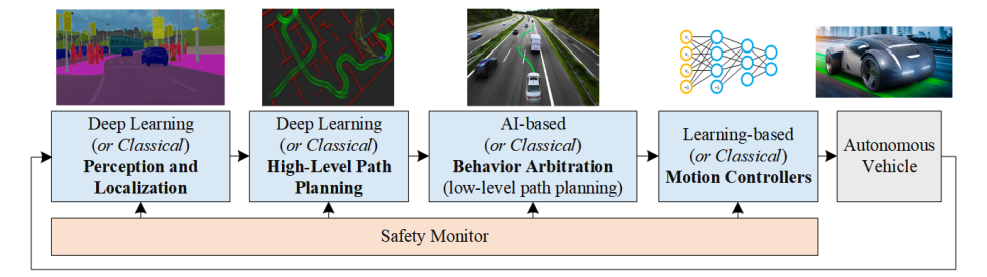
\includegraphics[keepaspectratio=true,width=6in]{figures/autonomous_driving_modular_pipeline.png}
    \caption{Deep Learning Based Autonomous Driving Modular Pipeline \cite{grigorescu_trasnea_cocias_macesanu_2020}}
    \label{fig:autonomous_driving_pipeline}
\end{figure}

To identify which module or modules are at fault, we need to understand and analyze each module of the modular pipeline. In this paper, we will only look at Perception and Localization, the first module in the autonomous vehicle pipeline. The Perception and Localization module is responsible for answering two questions: "Where is the car?" and "What is around the car?" \cite{liu_2020}. To perform this function, the module needs to utilize the sensing hardware and the software to understand the scene. Such hardware can be LiDAR, cameras, or other sensors. Nonetheless, they are all used for getting the information surround the vehicle and feeding those data to the software functionality of the module.

Getting the information surround the vehicle is straightforward as it simply records and passes those recorded data to the software functionality. However, understanding the scene is a more challenging task and not as straightforward. Unlike human beings, the machine sees and processes objects differently from our eyes and brain. While we see the object as a whole, the machine sees it as a grid of values that do not have any connection with one another. For this reason, the Computer Vision field tackles this problem and tries to create algorithms that are able to make sense of the object representation beyond the raw numerical data. The most important groups of algorithms in the Computer Vision field for understanding traffic scenes are video segmentation algorithms.

There are two types of video segmentation exist. The two are video semantic segmentation and video instance segmentation. In the video semantic segmentation algorithm, for each scene, objects in the scene are grouped and classified based on categories. On the other hand, video instance segmentation detects each instance of each category for each scene. Comparing semantic segmentation and instance segmentation, we can see that instance segmentation proposes a higher accuracy as it is able to see each instance of a class. That is, the instance segmentation algorithm will be able to distinguish between a car, a truck, and a bicycle if present instead of just vehicles class like semantic segmentation.

Since video instance segmentation algorithms give higher detection accuracy, in this paper, we will assume an algorithm from this group will be used for the Perception and Localization module. Knowing a video is a sequence of images, many video instance segmentation algorithms were proposed based on an algorithm in image instance segmentation. One example of such an algorithm is MaskTrack R-CNN which includes a new tracking branch to the well-known image instance segmentation Mask R-CNN. For that reason, to understand video instance segmentation, we first need to understand and analyze image instance segmentation. More specifically, this paper will discuss the building block of image instance segmentation algorithms. We then analyze and compare the performance of two well-known image instance segmentation algorithms, the Mask R-CNN and You Only Look Once version 7 (YOLOv7). Furthermore, we will want to identify if misidentified by these image instance segmentation algorithms causes the autonomous driving pipeline to fail and result in accidents.

%!TEX root = ../username.tex
\chapter{Neural Network} \label{chap:neural_network}

The group of Instance segmentation algorithms is a subgroup of object detection algorithms. All algorithms in the object detection group are required to do two tasks \cite{overview_cv_task}. 
\begin{enumerate}
    \item Generates a bounding box surrounding each object in the image.
    \item Classify the object in the bounding box.
\end{enumerate}
We first discuss the algorithm used for the classification task. Since in each bounding box, there is exactly one object to classify, an algorithm from the image classification task, a subset of the computer vision task, is applied \cite{overview_cv_task}.

% \hl{Conventional ML technique + limitation} \color{red} might put in the
% first para of NN section \color{black}
In the early day, as the first step toward artificial intelligence, a machine learning approach was proposed for the image classification task, but most were still designed manually by humans \cite{traditional_machine_learning}. Conventional machine learning uses feature extraction functions to map raw data to feature vectors. The feature vector is the only suitable data format that allows the learning subsystem of machine learning to detect patterns and classify the input. For that reason, the accuracy and effectiveness of machine learning methods are heavily dependent on the feature extraction function. However, the feature extraction function's responsibility is to extract features unique to the object that the machine tries to detect. Thus, the function requires an extremely detailed design and immense domain expertise to extract the feature of one object. Another disadvantage is that each object requires a different feature extraction function as they have unique features \cite{traditional_machine_learning}. The variety in features between objects causes the engineer to redesign the entire machine-learning architecture for each object which is a difficult task and inefficient.

% \hl{The paper outline}
As more studies go into the field, we start to move away from manually designed machine-learning methods to a more data-driven model. This data-driven algorithm group is now known as the artificial neural network.

% \hl{What is neural network}
Neural networks, also known as artificial neural networks (ANNs), are inspired by the human brain. Similar to the way the human brain processes and makes decisions, ANN is the core process of machine learning that gives the machine the ability to interpret the representation of raw binary data and move it toward artificial intelligence. An ANN algorithm is driven by data, the more data is supplied to the algorithm, the more accurate its interpretation ability becomes \cite{ai_data_driven}.

% \hl{Diff NN archietecture}
At the highest level of abstraction of ANN, there are two kinds of neural network architectures. The first and simplest one is feedforward architecture which allows its signal to travel from input to output \cite{lecun2015deep}. The feedforward network is widely utilized in grid patterns processing tasks, like image and video frames. The second architecture is the recurrent neural network (RNN). RNN expands the feedforward network's functionality by adding feedback connections that allow the network to feed its output back to the network \cite{lecun2015deep}. Feedback connections enable RNNs to be sufficient for processing sequences of data tasks.

% \hl{Hook to FC feedforward NN}
As this paper's interest lies in detecting objects of a scene, which require classifying individual objects in a grid of pixel values, we will only discuss the detail of a fully connected feedforward neural network.

\section{Feedforward Neural Network Architecture} \label{sec:feedforward_nn}

\begin{figure}[!ht]
    \centering
    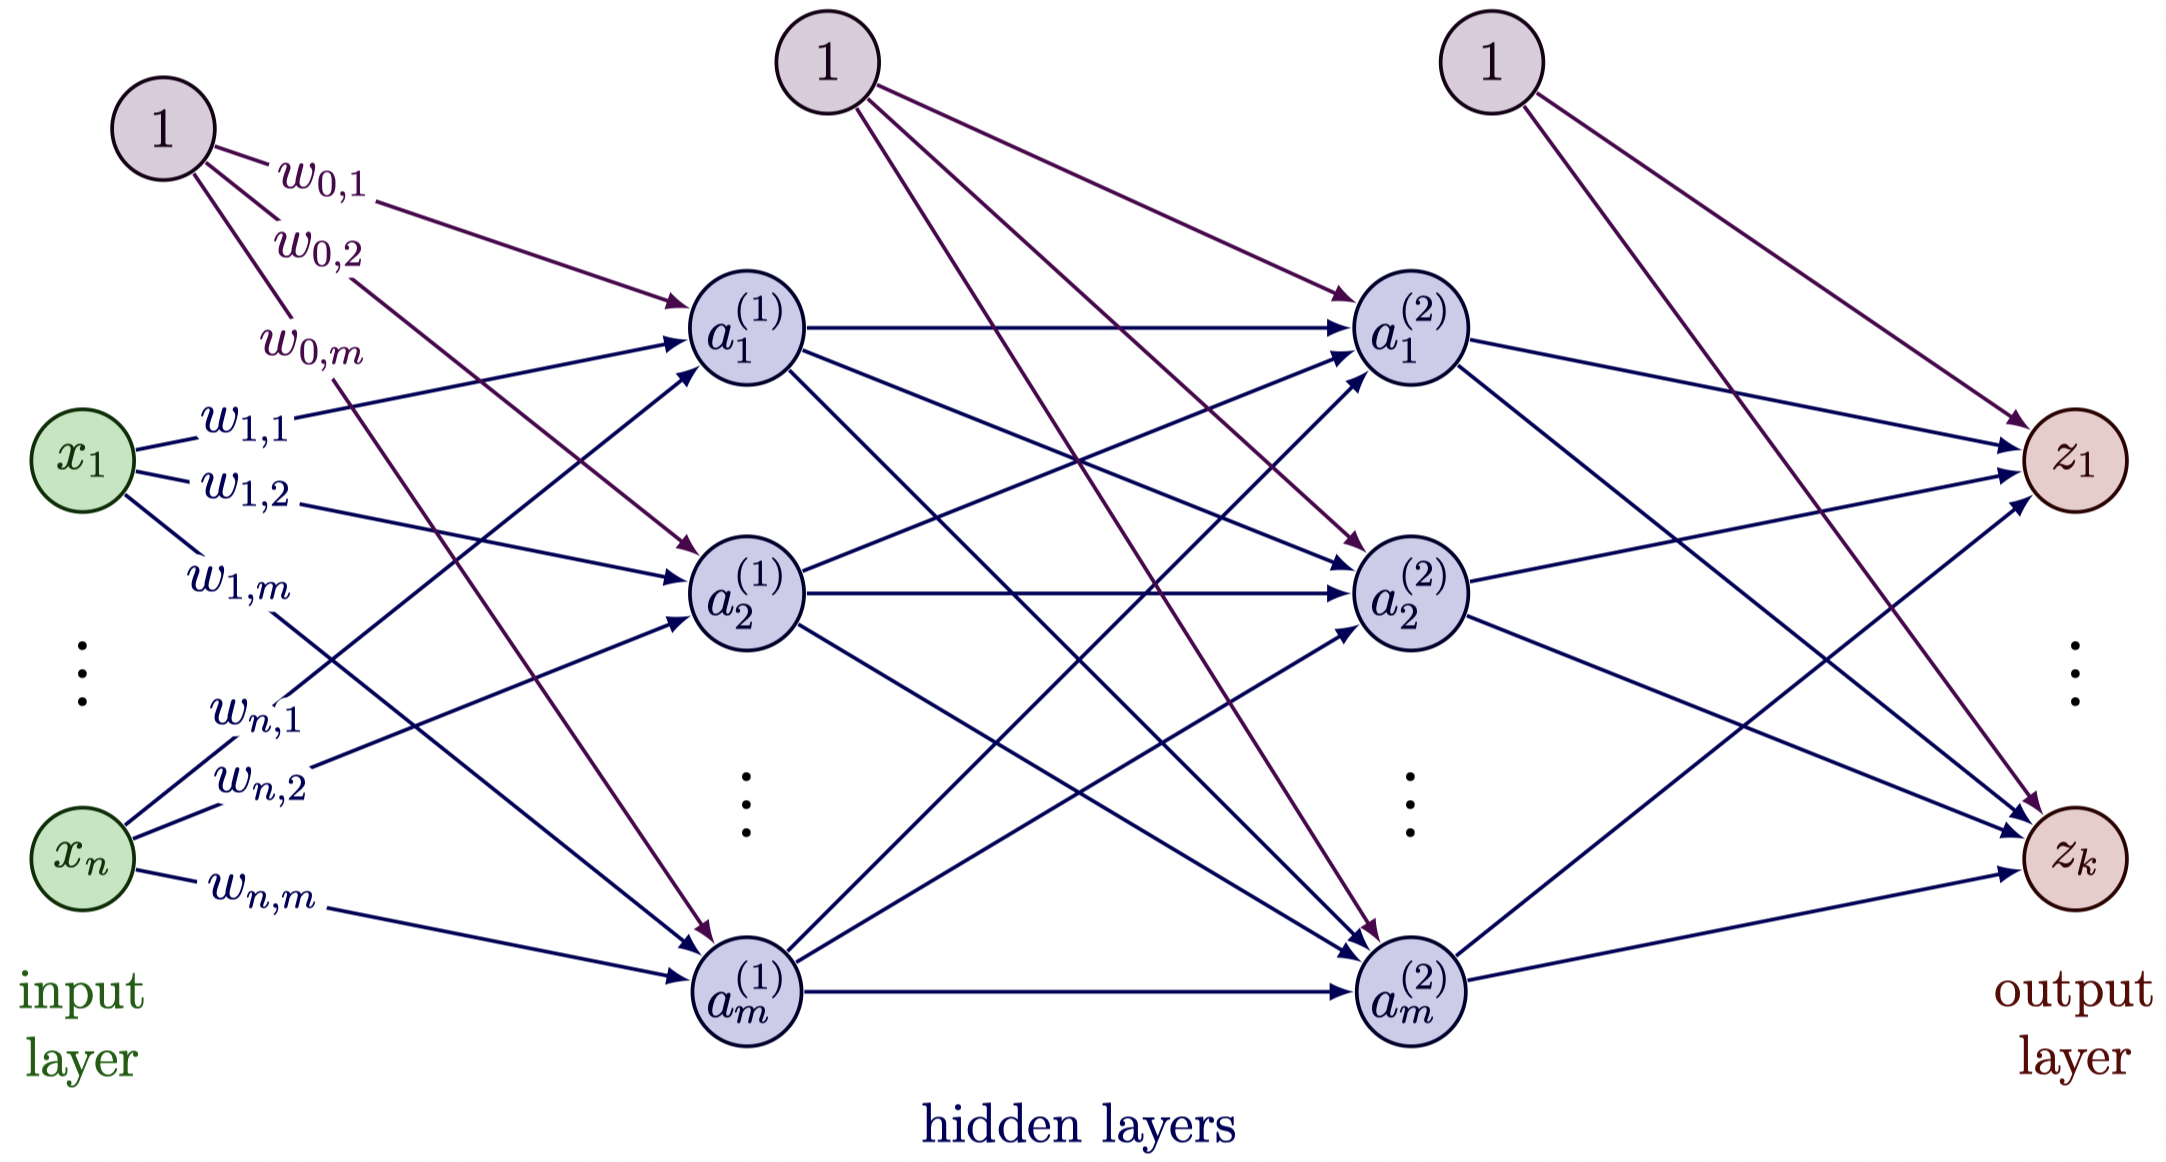
\includegraphics[width=5in]{figures/ffn_diagram.png}
    \caption{A Fully Connected Feedforward Neural Network} \label{fig:fc_ffn}
\end{figure}

Feedforward neural networks are the most basic type of deep learning model. Feedforward networks are designed to approximate a function that best maps the network's input to its output \cite{lecun2015deep}. On a high level, a feedforward neural network algorithm can be decomposed into four phases. The first phase is forward propagation, where the data flows through the network and initializes every node's values. The second phase is error evaluation, which determines how well the network does with its current setup. The third phase is gradient descent, where the algorithm determines which part of the network cause it to perform poorly. The last phase is backpropagation, where the algorithm updates the internal part of the network to make it more accurate and better fit the input data set. These four phases are applied and repeated on an extensive data set to become more precise over time. We will discuss more about each phase of the algorithm in this section, but we first need to understand the basic structure of a feedforward neural network.

\subsection{The Network Structure \label{network_structure}}
% \hl{Network layer}
To understand the feedforward network structure, we first need to define the idea of layers in the context of ANN. A \textbf{layer} in a neural network is a collection of neuron nodes at a specific network depth. A layer is represented by a column of node in Figure \ref{fig:fc_ffn}. A feedforward network can be thought of as a stack of multiple layers. Each layer in the stack is responsible for transforming the layer's input to help make sense part of the representation for later layers. On a high level, the network consists of the \textbf{input layer}, single or multiple \textbf{hidden layers}, and the \textbf{output layer}. The number of hidden and output layers is the \textbf{depth} of the network. As an example, Figure \ref{fig:fc_ffn} is a fully connected feedforward neural network with a depth of three.

% \hl{Network neuron + activation signal}
Each layer consist of one or more nodes. Each node in a layer represents an \textbf{artificial neuron}. The number of neurons in each layer can be different from one another. Each neuron holds a numerical value called the \textbf{activation signal}. In theory, the activation signal takes on any value in the real numbers set $\mathbb{R}$. However, in practice, studies have shown multiple advantages, {\color{red} like improved training time and avoiding overfitting problems [section 2.3]}, when normalizing the activation signal of every neuron \cite{lecun2012efficient}. As an example, we consider a network that receives a $23 \times 23$ RGB image and then produces a dog or cat label for the object in the image. In the input layer, the number of neurons is the total pixel in the image in each color channel, that is $23 \times 23 \times 3$ neurons, and each neuron (denoted $x_i$) holds that pixel value normalized. On the other hand, the output layer only has two neurons (denoted $z_i$); one corresponds with the dog and the other with the cat. Unlike the input and output layer, where the number of neurons needed is straightforward, the number of neurons in each hidden layer and the number of hidden layers are complicated to determine and remain outside the scope of this paper. However, studies have shown that networks with the same neurons' hidden layers perform better \cite{taylor2017neural}, and deeper networks result in more advanced learning with some issues like gradient vanishing and more {\color{red} [section 2.3]}. {\color{red} Discuss overfiting and gradient vanishing problem in section 2.3}

% \hl{Network connection + weight}
Each neuron in a layer can affect a neuron from the next layer through a \textbf{connection}. The connection is represented by a line between two neurons in Figure \ref{fig:fc_ffn}. In fully connected networks, each neuron in a layer will be affected by all the neurons from the previous layer. In other words, each neuron will have a connection with every neuron in the previous and next layer of the network. Associate with each connection is a numerical value representing the \textbf{weight}. The weight of a neuron infers how influence the neuron will be on the next layer of the neural network. A small weight value means the activation signal of this neuron has a low effect on neurons of the next layer. On the other hand, a high weight value results in a more significant effect proposed by this neuron to the next layer and the network's output. When a neural network algorithm initialize, its weights are randomly assigned using a Gaussian or uniform distribution \cite{lecun2015deep}. {\color{red} Discuss Gaussian or uniform distribution in section 2.3} These weights are adjusted as the neural network algorithm process to best approximate its mapping function. The weight from neuron $a_i$ to a neuron $a_j$ in the next layer will be denoted as $w_{i,j}$ with the exception of bias's weight.

% \hl{Network bias}
In addition to the weight, neurons in each layer other than the input layer are also influenced by a \textbf{bias node}. A bias node is represented by a node that always holds value 1. The bias node has connections to every neuron in the layer it affects. Each bias's connection also has a weight associated with it. The connection between bias and neuron $a_j$ in the affected layer will have its weight denoted as $w_{0,j}$. The role of the bias node is like a threshold to the neuron. In other words, the bias determines how significant the activation signal of a neuron must be before that neuron gets propagated to the next layer of the network. Similar to weight, when the network initializes, the bias's weight is randomly assigned a value, and this value is optimized as the algorithm process. In the forward process of the network, the algorithm will compute a net input that requires a multiplication between a neuron activation signal and its weight. Since the bias node always has an activation signal of 1, thus the bias weight is the variable that directly affects nodes in the next layer. Therefore, the bias's weight is often refers as the bias.

These basic building blocks create the internal structure of a feedforward neural network. Some internal parts are also known as internal variables or network parameters. The model parameters refer to variables that are learnable in the gradient descent process, and they are not set manually by the developers. Weights and bias weights are examples of the network's parameters. In contrast with parameters, hyperparameter refers to variables manually set by the developers and sometimes can be optimized through training. Examples of hyperparameters are the learning rate and batch size, which we will touch on more in the gradient descent section.

% \hl{Hook to forward propagation}
With the basic structure of the fully connected feedforward neural network in mind, we will discuss the first phase of an ANN algorithm. That phase is forward propagation.

\subsection{Forward Propagation} \label{forwardprop_section}
Forward propagation refers to the process by which the data move from the input layer to the output layer of the network. Regarding the image classification problem, the forward propagation process moves a list of raw pixel values through the network and gives out a number for each class label. These numbers are the \textbf{network's raw ouput}, and each number represents how likely the image is a member of this class. The forward propagation process uses two functions to evaluate the activation signal of each neuron in hidden and output layers. These two function are the \textbf{summation function} and the \textbf{activation function} \cite{taylor2017neural}.

\begin{wrapfigure}{l}{2.5in}
    \centering
    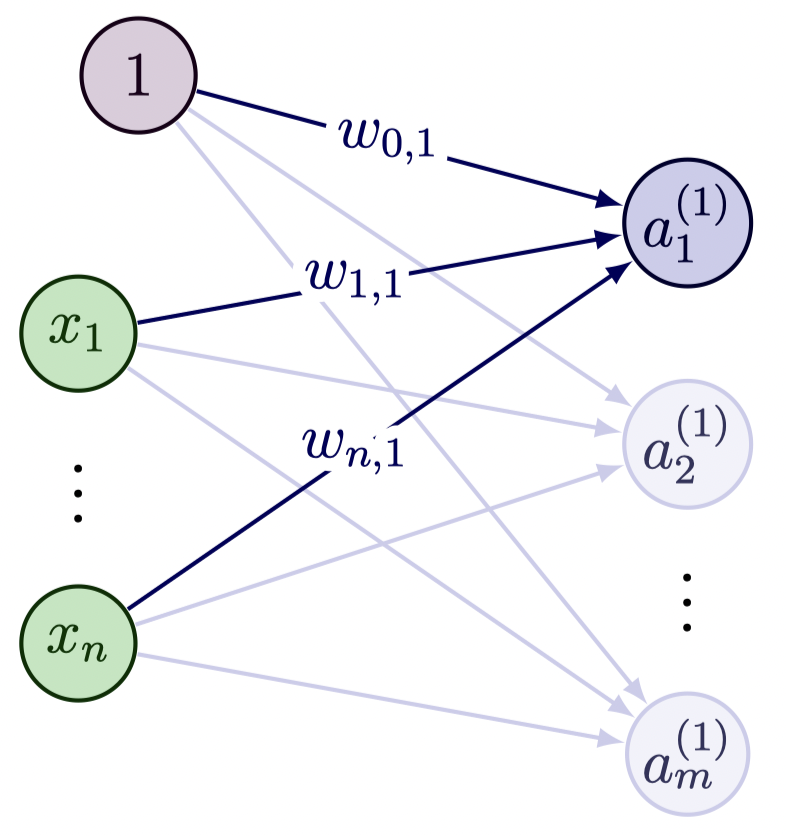
\includegraphics[width=2in]{figures/fp_diagram.png}
\end{wrapfigure}

% \hl{Summation function}
\noindent In a fully connected network, the summation function combines all neurons and their weight from the previous layer to create the net input for the current neuron. In general, the summation function can be expressed as \[net\ input\ of\ a_j = \sum_{i=1}^n (x_i w_{i,j}) + 1 \cdot w_{0,j}\] where $a_j$ represents the neuron that has the summation function compute its net input. The neuron's net input will then be transformed by an activation function.

% \hl{Activation func}
The activation function is responsible for transforming the net input into an activation signal, indicating if this neuron will affect later network layers. Additionally, linear functions are closed under addition, that is, adding or subtracting multiple linear functions from or to another function will result in a linear function. This fact implied that the feedforward network must have non-linearity terms if it approximates a non-linear function. The use of the activation function enables the network to introduce non-linearity terms to the algorithm. Furthermore, studies have shown that the output of a network - a network that only uses a linear activation function or does not use an activation function - will be a linear combination of its input, which means hidden layers have no effect \cite{He_2015_ICCV}.

% \hl{Most common activation function} 
There are numerous activation functions proposed, each with different strengths and weaknesses. However, in practice, there are four functions and their variance that are widely used by the ANN algorithm. These four activation functions are the linear, sigmoid, hyperbolic tangent (tanh), and rectified linear unit (ReLU). The formula and graphical representation of each function are shown in Table \ref{acti_func_table}.

\begin{figure}[!ht]
    \centering
    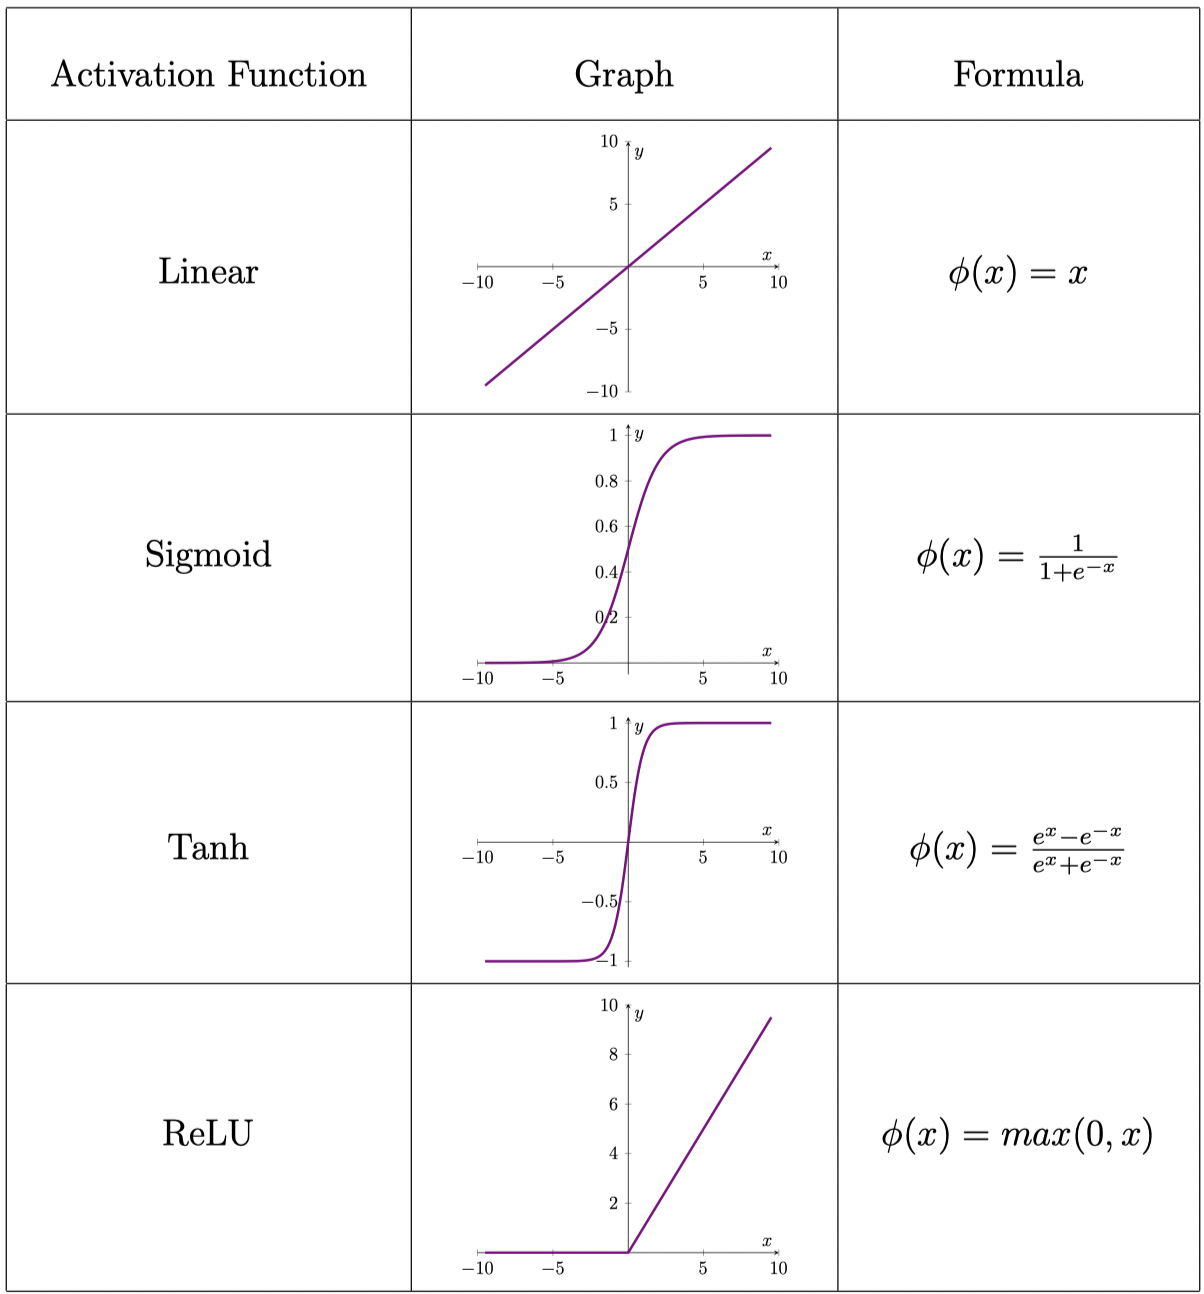
\includegraphics[width=5in]{figures/acti_func_table.png}
    \caption{Most Common Activation Function}
    \label{acti_func_table}
\end{figure}

% \hl{Activation func strength + weakness - need rewrite?} 
To understand which activation function to choose for a network, we need to know some important strengths and weaknesses of each function. First of all, the linear function is simple; thus, it forgiving and undemanding about the resources required for training. However, the linear function is close under addition; thus, the network will only be able to approximate a linear mapping function. In contrast, sigmoid and tanh are non-linear functions, thus allowing the network to approximate a non-linear mapping function. Additionally, sigmoid and tanh map real number set to (0, 1) and (-1, 1), respectively. The mapping of sigmoid and tanh allow the activation signal to be normalized, thus improving training time and avoiding exploding gradients \cite{lecun2015deep} {\color{red} [section 2.3]}. However, the mapping also causes sigmoid and tanh to suffer from the vanishing gradients problems. Different from sigmoid and tanh, ReLU map positive signal to itself, thus able to avoid the vanishing gradients problems. The first disadvantage of ReLU is it does not have any upper bound, which require the network to have some additional nomalization layer like batch normalzation (BN), weight normalizaiton (WN), and layer normalizaiton (LN) to optimize the training process \cite{relu_optimization_2020} {\color{red} [section 2.3]}. The second disadvantage of ReLU is it suffer from the dying ReLU problem which cause by the fact that all negative signal is map to 0 {\color{red} [section 2.3]}. Despite the dying ReLU problem, ReLU proves to be very efficient and accurate in practice; thus, it is the most used activation function currently \cite{li2021survey}. Furthermore, some variance of ReLU has been proposed to avoid the dying ReLU problem like Leaky ReLU and ELU. The problems possessed by these activation function is crucial when it comes to choosing an activation function and can be read more at LeCun et al., \cite{lecun2015deep}.

\subsection{Error Evaluation}
Once the forward propagation is completed, the algorithm will need to determine the correctness of the network with the current weight and bias. In order to estimate the network's correctness, the algorithm computes the difference between the network's output and the expected output. This process is known as the \textbf{error evaluation phase}, and it uses a \textbf{loss function} to quantify the difference. The three most used loss functions are \textbf{Mean Absolute Error} (MAE), \textbf{Mean Square Error} (MSE), and \textbf{Cross-Entropy}. MAE and MSE are primarily used in regression problems, while Cross-Entropy is mainly used in classification problems \cite{li2021survey}. As the focus of this paper is on the image classification task, we will only focus on Cross-Entropy.

Cross-Entropy is a loss function that is always used in conjunction with a softmax layer. A \textbf{softmax layer} is a layer that has the same number of nodes as the network's output layer. The goal of a softmax layer is to transform the raw output into probabilities for classes in the network's output, denoted $\hat{y}$. In other words, each neuron node activation signal is a class's probability after the softmax layer and is bounded by 0 and 1; and the probabilities of all classes must add to 1. The softmax layer use a softmax function to map a raw output value to the range $0-1$. The \textbf{softmax function} is defined as follow:
\[
    \hat{y_i} = \sigma(z_i)=\frac{e^{z_i}}{\sum^k_{j=1}e^{z_j}} \text{ \qquad
    with } i = 1, 2, 3, ... , k
\] 
where $z_1, z_2, z_3, ... , z_k$ are the value of network's raw output. The use of a softmax layer is crucial for output interpretation. Since a raw output does not have a lower or an upper bound for its value, thus different image might result in a different value range for the class label. This wide range of value behavior makes the raw output extremely hard to interpret and compare with the output of other images. The softmax layer standardizes the output by mapping the raw output to the range $0-1$ before comparing and calculating the error.

% \hl{cross-entropy loss} 
The softmax layer enables us to represent the network's output as a probability distribution for the object's class with a higher value means the object is more likely to be a member of that class. Similarly, we can also represent our desired classification output as a probability distribution with 1 for the object's class and 0 for all other classes. With that in mind, we have the Cross-Entropy function able to quantify the difference between two probability distributions, thus we use it to determine how far the network's output is from the actual desired output. The Cross-Entropy value of a standardized output neuron can be computed as follow: \[\text{CE of }\hat{y}_i = -\sum^k_{i=1} t_i \times \log(\hat{y}_i)\] where $t_i$ is the expected class$_i$'s value for the object present in our input image and $\hat{y}_i$ is the class$_i$'s probability for the object predicted by the network.

The Cross-Entropy for a neuron above describes the distance between the neuron's current activation signal and its expected value. By computing the Cross-Entropy for every output neurons, the sum of these Cross-Entropy values gives us the total error of the network. That is, the total Cross-Entropy describes how far the network is from its expected output in a single value and can be formularized as follow:
\[
    \text{Total Cross-Entropy} = \sum^k_{i=1} \text{Cross-Entropy of }\hat{y}_i
\]
where $k$ is the number of output neurons i.e. the number of class that we are trying to classify. Since total Cross-Entropy gives us a single value to describe the total error in the network, thus by reducing the total Cross-Entropy value, the network will become more accurate. This concept of reducing the total Cross-Entropy value to make the neural network more accurate is the core idea of gradient descent.

\subsection{Gradient Descent}
\textbf{Gradient descent} is an optimization process in which our feedforward network evaluates how the network's parameters affect total error, thus giving insight on how to reduce the total error. An ANN can have two or more parameters depending on the model; however, there are two that exist in any ANN model: weight and bias's weight. For simplicity, let us assume our network only has two learnable parameters -- weight and bias. If we were to plot the total Cross-Entropy as a function of weight and bias in 3D space, we would result in a 3D surface that describes the total Cross-Entropy values at different combinations of weight and bias. The idea of gradient descent is to have the network's total Cross-Entropy value moving toward the global minimum, which will use a specific combination of weight and bias. There are three types of gradient descent methods; to understand those, we first define the idea of an epoch, batch, and iteration.
%
\begin{itemize}
    \item An \textbf{epoch} refer to when the network see the entire training data set exact one time.
    \item A \textbf{batch} is the number of example that pass through the network exact one before updating the network's parameters.
    \item An \textbf{iteration} refer to number of time a batch of data need to pass through a network to complete an epoch. This also state the number update for an epoch.
\end{itemize}
%
As an example, if our image classification training data set have 1000 images with the batch size of 250, then we need 4 iteration to pass the entire training set throught the network and complete one epoch.

The three types of gradient descent are \textbf{Full-Batch Gradient Descent} (BGD), \textbf{Stoc-hastic Gradient Descent} (SGD), and \textbf{Mini-Batch Gradient Descent} (MGD). Each method impacts when the weight and bias will be updated during training, thus resulting in different pros and cons.

% \hl{BGD} 
The first gradient descent method is BGD which is a one iteration method. Since BGD only updates weight and bias after an epoch, it is undoubtedly the slowest of the three in terms of training time. However, by having the batch size equal to an epoch, BGD guaranteed to find a global minimum on the Cross-Entropy 3D convex surface. Thus BGD enables the network to adjust the weight and bias to move toward the optimal solution over each epoch.

% \hl{SGD}
The second gradient descent method is SGD which is an $n$ iteration method where $n$ is the number of training examples in one epoch. Since SGD updates the weight and bias after each training example pass through the network; thus it is much faster in updating weight and bias than BGD. Despite having a faster update, SGD suffers from a high variance of training examples since improving error for one example does not equate to improving error for other examples in the training set. Hence, SGD is faster for large training sets but might never reach the global minimum of the loss function. As an additional note, using SGD requires the training set to be shuffled before input to the network as the order of example can introduce unknown bias to the model.

% \hl{MGD} 
The third and most used method nowadays is MGD. MGD has the advantage of both BGD and SGD as it allows the developer to choose the trade-off between training time and accuracy through batch size. \textbf{Batch size} is one of the network's hyperparameters which is bounded by 1 and $n$, where $n$ is the number of training examples in one epoch. A larger batch size moves the network behavior toward BGD behavior, while a smaller batch size will cause the network behavior to resemble SGD. Studies have shown the value of batch size should be a relatively small power of 2 bounded by 1 and a few hundred with a reasonable default value of 32 \cite{bengio2012practical, masters2018revisiting}. Some studies also propose the use of an adaptive batch size where the network starts with small batch size, then increases after each update \cite{lecun2012efficient}. However, the rate of increase of batch size in these proposals is still challenging to determine and generalize; thus, most successful networks still only use a fixed batch size.

% \hl{compute gradient} 
By choosing one of the three methods of gradient descent, we now know when the network's weights and bias get updated. To know how much the weights and biases need to be updated to bring the model closer to the global minimum of the loss function, we need to know how much a change in weight or bias affects a change in the loss function. For this reason, the algorithm uses partial derivate to quantify the rate of change of the total Cross-Entropy with respect to a change in a specific weight or bias. This process is also known as computing the gradient for each weight and bias in the network. The gradient for weight $j$ can be computed using the following formula:
\[
    \frac{\Delta \text{Tot. CE}}{\Delta w_j}= \sum^k_{i=1}\frac{\Delta \text{CE of }\hat{y}_i}{\Delta w_j}
\]
where $\hat{y}_1, \hat{y}_2, ..., \hat{y}_k$ are the standardized output of neurons affected by weight $w_j$. To understand how to evaluate the gradient, we consider a simple network show in Figure \ref{fig:gradient_nn}.
%
\begin{figure}[H]
    \centering
    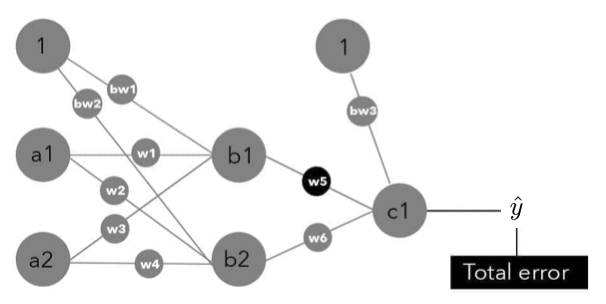
\includegraphics[width=3.5in]{figures/simple_nn_gradient.png}
    \caption{Simple Neural Network \cite{taylor2017neural}} \label{fig:gradient_nn}
\end{figure}

For this example, we will calculate the gradient of the weight $w_5$ and weight $w_1$. To calculate the gradient of weight $w_5$, we need to calculate the rate of change of the total Cross-Entropy with respect to weight $w_5$. Since this simple network only has one output neuron, denoted $c_1$, then the rate of change of total Cross-Entropy is the rate of change of the Cross-Entropy of $\hat{y}$, where $\hat{y}$ is the standardized value of output neuron $c_1$. Thus we have the gradient of weight $w_5$ as:
%
\begin{equation} \label{w5_eq1}
    \frac{\Delta \text{Tot. CE}}{\Delta w_5}= \frac{\Delta \text{CE of }\hat{y}}{\Delta w_5}
\end{equation}
%
However, weight $w_5$ does not affect the Cross-Entropy of $\hat{y}$ directly, but instead affects the net input of output neuron $c_1$, which intern affect the activation signal of $c_1$. Then and only then, output neuron $c_1$ affects the standardized value $\hat{y}$ and its Cross-Entropy. For that reason, to compute the gradient of weight $w_5$, we need to link weight $w_5$ to the Cross-Entropy of $\hat{y}$ by performing chain rule operations on the partial derivative. Apply chain rule to Equation \ref{w5_eq1} for weight $w_5$'s gradient, we have:
%
\begin{equation} \label{w5_eq2}
    \frac{\Delta \text{Tot. CE}}{\Delta w_5}
    = \frac{\Delta \text{CE of }\hat{y}}{\Delta \hat{y}}
    \times \frac{\Delta \hat{y}}{\Delta c_1}
    \times \frac{\Delta c_1}{\Delta c_1 \text{ net\_input}}
    \times \frac{\Delta c_1 \text{ net\_input}}{\Delta w_5}
\end{equation}
%
Similarly to weight $w_5$, the gradient of weight $w_1$ can also be computed using the partial derivative with the chain rule. Weight $w_1$ affects the net input of neuron $b_1$, then its activation signal. Then, Neuron $b_1$ impacts the net input of neuron $c_1$ and its activation signal. Neuron $c_1$ then affect $\hat{y}$ and its Cross-Entropy value. Notice that from neuron $c_1$ onward, the change is the same as part of weight $w_5$'s gradient formula; thus, we can expand and adapt Equation \ref{w5_eq2} to compute the gradient of weight $w_1$. The gradient of weight $w_1$ can be evaluated as follow:
%
\[
    \frac{\Delta \text{Tot. CE}}{\Delta w_1} = \frac{\Delta \text{CE of }\hat{y}}{\Delta \hat{y}} \times
    \frac{\Delta \hat{y}}{\Delta c_1} \times \frac{\Delta c_1}{\Delta c_1 \text{ netin}} \times \frac{\Delta c_1 \text{ netin}}{\Delta b_1}
    \times \frac{\Delta b_1}{\Delta b_1 \text{ netin}}
    \times \frac{\Delta b_1 \text{ netin}}{\Delta w_1}
\]
%
where "netin" stand for the net input. These examples showcase the computational process for the gradient of an in-network and an out-network weight i.e., $w_1$ and $w_5$, respectively. The same computation process for the gradient is applied to all network weights and biases, even with a more complex and higher depth network. Once the gradient is calculated for all the weights and biases, the algorithm knows how much a paticular weight or bias changes the network's total error, and thus ready to update each weight and bias accordingly.

\subsection{Backpropagation}
\textbf{Backpropagation} refer to a phase in which the algorithm using gradients of weight or bias to update their value and bring the network's total error to global minimum. Since the gradient give the slope of the loss function with respect to a weight or bias, and backpropagation update their value to approaching global minimum, thus gradient descent along with backpropagation process enable neural network to has a behavior similar to the idea of learning through the process of optimizing network's parameters. The formula to update the value of weight $w_j$ is:
%
\begin{equation} \label{backprop_func}
    \text{new } w_j = \text{old } w_j - \left( \frac{\Delta \text{Tot. CE}}{\Delta w_j} \times \eta \right)
\end{equation}
%
where old $w_j$ is the current value of weight $w_j$, $\frac{\Delta \text{Tot. CE}}{\Delta w_j}$ is the gradient of weight $w_j$, and $\eta$ refer to the algorithm's learning rate.

\textbf{Learning rate}, denoted $\eta$, is a network's hyperparameter and it determine how fast the network learn. In the updating weight function, equation \ref{backprop_func}, the learning rate directly affect the size of the step when the algorithm move toward global minimum for total error. Large leaning rate means bigger step toward minimum, thus result in faster learning, while smaller learning rate value result in slower leaning. However, a large leaning rate can also affect the network's ability to reach global minimum as it can over step and pass optimal value. Studies has shown value of a leaning rate for a multi-layer ANN should be between $10^{-16}$ and 1 with a reasonable default value of 0.01 \cite{bengio2012practical}. {\color{red} Consider put the learning rate paragraph into [section 2.3]}

As the backpropagation phase is completed, all weights and biases in the network get updated, and all four phases of the algorithm are repeated on the next batch, where the size of each batch depends on the method of gradient descent. These phases are repeated until the algorithm's total error function reaches a global minimum. At that moment, a test set will be passed through the network, and the network's total error will be returned to determine the accuracy of the algorithm.


% !TEX root = ../../username.tex
\section{Convolutional Neural Network} \label{sec:cnn}

\textbf{Convolutional Neural Network} (CNN) is a type of feedforward neural network designed to process images. A simple structure of a CNN consists of five types of layers. These layers are the input, convolutional, pooling, fully connected, and output layers. The fully connected layer is responsible for the actual classification process. Both fully connected and output layers behave the same as in a fully connected feedforward network discussed in Section \ref{sec:feedforward_nn}. A simple CNN structure for handwritten digit classification is shown in Figure \ref{fig:simple_cnn_diagram}.

\begin{figure}[!ht]
    \centering
    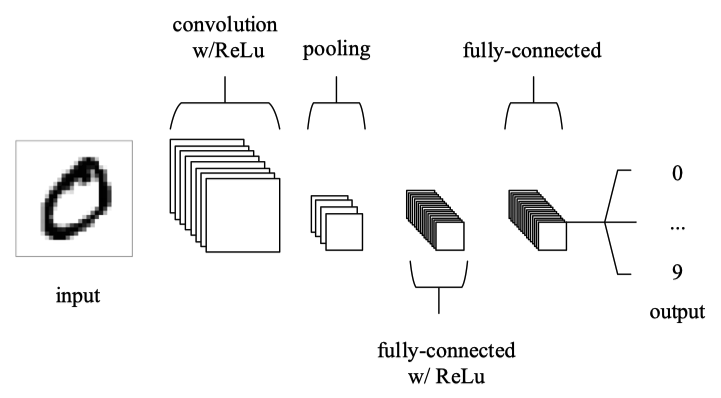
\includegraphics[width=4.5in]{figures/simple_cnn.png}
    \caption{Simple CNN structure for handwritten digit classification \cite{o2015introduction}}
    \label{fig:simple_cnn_diagram}
\end{figure}

Since an image is a 2D grid pattern data, it is possible to flatten the image and pass it through a fully connected feedforward neural network for classification directly. However, there are multiple benefits when using CNN over a standard feedforward network. The two most important benefits of CNN are spatial interaction capturing and data downsampling.

The first significant benefit is spatial interaction. \textbf{Spatial interaction} in an image refers to the connection between two or more pixel values. These connections are essential since pixels next to one another tend to describe a feature of an object, while pixels far from each other describe a different feature of the same object or a completely different object; thus, spatial interaction enhances feature extraction. On the other hand, if an image is flattened, pixels that appear close to one another will be very far away in the network, thus losing their meaning.

The second important benefit is data downsampling. \textbf{Data downsampling} refers to reducing the number of weights in the network. Consider a $64 \times 64$ RGB image, in a fully connected feedforward network, each neuron in the network will need to consider value from $64 \times 64 \times 3 = 12,288$ neurons from the previous layer. In other words, each neuron will have $12,288$ incoming connections, and the network needs to compute the gradient and do backpropagation for $12,288$ weights per neuron per network's layer. Thus, the computational and memory usage are still expensive despite the image being a low-resolution photo. Therefore, if a network could downsampling the data, it would be more efficient, have less training time, and require less computational power.

CNN is able to capture the spatial interaction and perform data downsampling using the convolutional and pooling layer before passing to a fully connected layer for classification. To further understand CNN structure, we will discuss convolutional and pooling layer functionality in detail.

\subsection{Convolutional Layer}
\textbf{Convolutional layer} is responsible for making the spatial connection and extracting features from the image. These tasks can be achieved with the use of learnable kernels. A kernel is a grid of data that has a smaller width and height but has the same depth as the input image. For example, a $64 \times 64$ RGB image will require the kernel to have the size of $x \times x \times 3$ where $x$ bounded by $2$ and $64$ inclusively. There are various types of kernels, and each type is designed to target a specific task. These tasks include blurring, sharpening, edge detection, and more. When applying the kernel to the input image, it slides from left to right and top to bottom. As it slides, the kernel's activation signal is computed by performing a scalar product of the kernel with the subregion of the image covered by it, as shown in Figure \ref{fig:kernel_op_diagram}. The kernel's activation signal represents how likely the feature -- the feature that the kernel is trying to extract -- is present at the current spatial position of the input image. The resulting grid of the kernel's activation signal is the feature map. Each kernel has an associate activation map. If multiple kernels are applied to an image, then the output feature map of these kernels will be stacked along the depth dimension.

% The kernel value are predefine for specific task. This is possible purely base on the mathematics of convolution operator. For example, a kernel with values follow the gaudience distribution, then it will give the center the kernel the highest value, and get smaller as we approach the edge of the kernel. But since the center value is effect by the value of pixels arround it, thus the sum of these make the center pixel blended in with pixels around it. Create the blurring effect.

\begin{figure}[!ht]
    \centering
    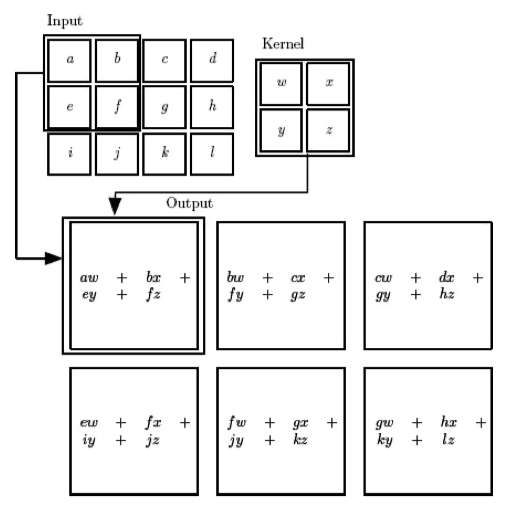
\includegraphics[width=3.5in]{figures/kernel_operation.png}
    \caption{Scalar product for a kernel's activation signal \cite{lecun2015deep}} 
    \label{fig:kernel_op_diagram}
\end{figure}
%
Notice that a kernel's width and height must be equal, and the kernel itself must be symmetric. Studies have shown that using symmetric kernels enables the algorithm to extract the inverse of a feature, thus improving the generalization for feature extraction. Additionally, since the kernel's activation signal is only based on a subregion of the image that the kernel applied to, this kernel neuron will only be connected with the neurons associated with pixels in this subregion in the network, thus reducing the number of weight in the network. The width and height of this subregion are also known as the receptive field size. Reconsider our $64 \times 64$ RGB image example, if the recaptive field is $4$, then each neuron will only have $4 \times 4 \times 3 = 48$ connections. Thus, the network will only need to compute gradient descent and do backpropagation for $48$ weights for this neuron instead of $12,288$ weights.

Other than width and height, we can also change the stride and the zero-padding to fine-tune the kernel behavior. The stride enables the kernel to slide through the image with a more significant step. That is, if the stride is 1, then the kernel will move to the left and down one pixel at a time and calculate the kernel's activation signal. Besides the stride, zero-padding also changes the convolutional behavior. The zero-padding value is the number of zero rows and columns surrounding the border of the input image. The zero-padding allows the algorithm to emphasize the border of the input image. Along with stride and zero-padding, we denoted a kernel as 
\[
    \text{kernel width} \times \text{kernel height, zero-pading size, /stride value}
\]
An the feature map size can be computed as follow:
%
\begin{equation} \label{feature_size_eq}
    \text{feature size} = \left(\frac{(\text{image size} - \text{kernel size}) + 2 \times \text{padding size}}{\text{stride}} \right) + 1
\end{equation}

\subsection{Pooling Layer}
Unlike the convolutional layer, the pooling layer only has one purpose: reducing the number of neurons in the network. The use of the pooling layer help result in fewer parameters for the network and thus require less computational power. Similar to the kernel, the pooling layer also slide through a grid of value. However, instead of sliding through the input image, the pooling layer slides through the feature map or the convoluted image to reduce the size of the feature map. There are two types of pooling layers, and they are max-pool and average-pool. As the name suggested, a max-pool layer will extract the largest activation signal in a subregion of the feature map while removing all other activation signals in the same subregion. An example of a max-pool function is shown in Figure \ref{fig:max_pool_diagram}. On the other hand, an average-pool layer takes the average value of all the activation signals in the subregion. The choice of which pooling layer to use depends on whether we care about every feature in the image equally, then the average-pool is used, or if we only care about the more prominent feature, then max-pool is used. Pooling also uses the stride to change how big of the step the pooling layer will slide through the feature map, denoted $/x$ where $x$ is stride value.
%
\begin{figure}[!ht]
    \centering
    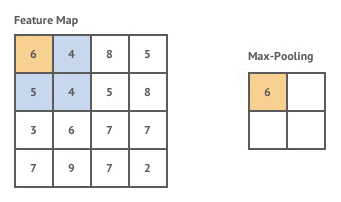
\includegraphics[width=3.5in]{figures/max_pool.png}
    \caption{$2 \times 2,\ /2$ max-pool on \cite{zeiler2014visualizing}}
    \label{fig:max_pool_diagram}
\end{figure}
%
Since pooling layer also slide throught a grid of value and output exactly one value for the subregion, thus a similar function to Equation \ref{feature_size_eq} is used to calculate the output size for pooling layer. The output size can be calculate as follow:
\[
    \text{pooling's output size} = \left(\frac{(\text{feature size} - \text{pooling size})}{\text{stride}} \right) + 1
\]

As an example, reconsider our $64 \times 64$ RGB image example, by applying a $4 \times 4, 0, \ /1$ kernel and a $2 \times 2,\ /2$ max-pool layer, the convoluted image size before passing to fully connected layer for classification is:
\[
    \text{output size} = \left[ \left( \frac{(64 - 4) + 2 \times 0}{1} + 1 \right) - 2 \right] \times \frac{1}{2} + 1 = 30 
\] 
Thus, the algorithm able to reduce from $12,288$ weights to $30 \times 30 \times 3 = 2700$ weights. In practice, it is common to have more than one kernel and one ouput apply to an input image.

% \hl{note}
% - what does NN do?
% - who came up with the idea (1-2 sentences)
% - basic des of NN architecture
% - what is limitation of NN

% Therefore, the kernel able to perform feature extraction with spatial
% connection and reduce the number of connection per neuron.
%!TEX root = ../username.tex
\chapter{Computer Vision Tasks And Evaluation Metrics} \label{chap:segmentation_metric}

\section{Object Detection, Instance Segmentation, and Other Tasks}  \label{sec:cv_tasks}

The field of computer vision aims to enable machines the ability to comprehend and derive meaning from visual scenes. This field comprises several tasks for processing images and videos, including but not limited to image classification, object detection, semantic segmentation, and instance segmentation \cite{overview_cv_task}. However, for the purpose of our study, we will focus specifically on object detection and instance segmentation. In this section, we will define these two tasks, then compare them with related tasks such as image classification and semantic segmentation. Followed by a discussion of the metrics used to evaluate object detection and instance segmentation models.

\begin{figure}[!ht]
    \centering
    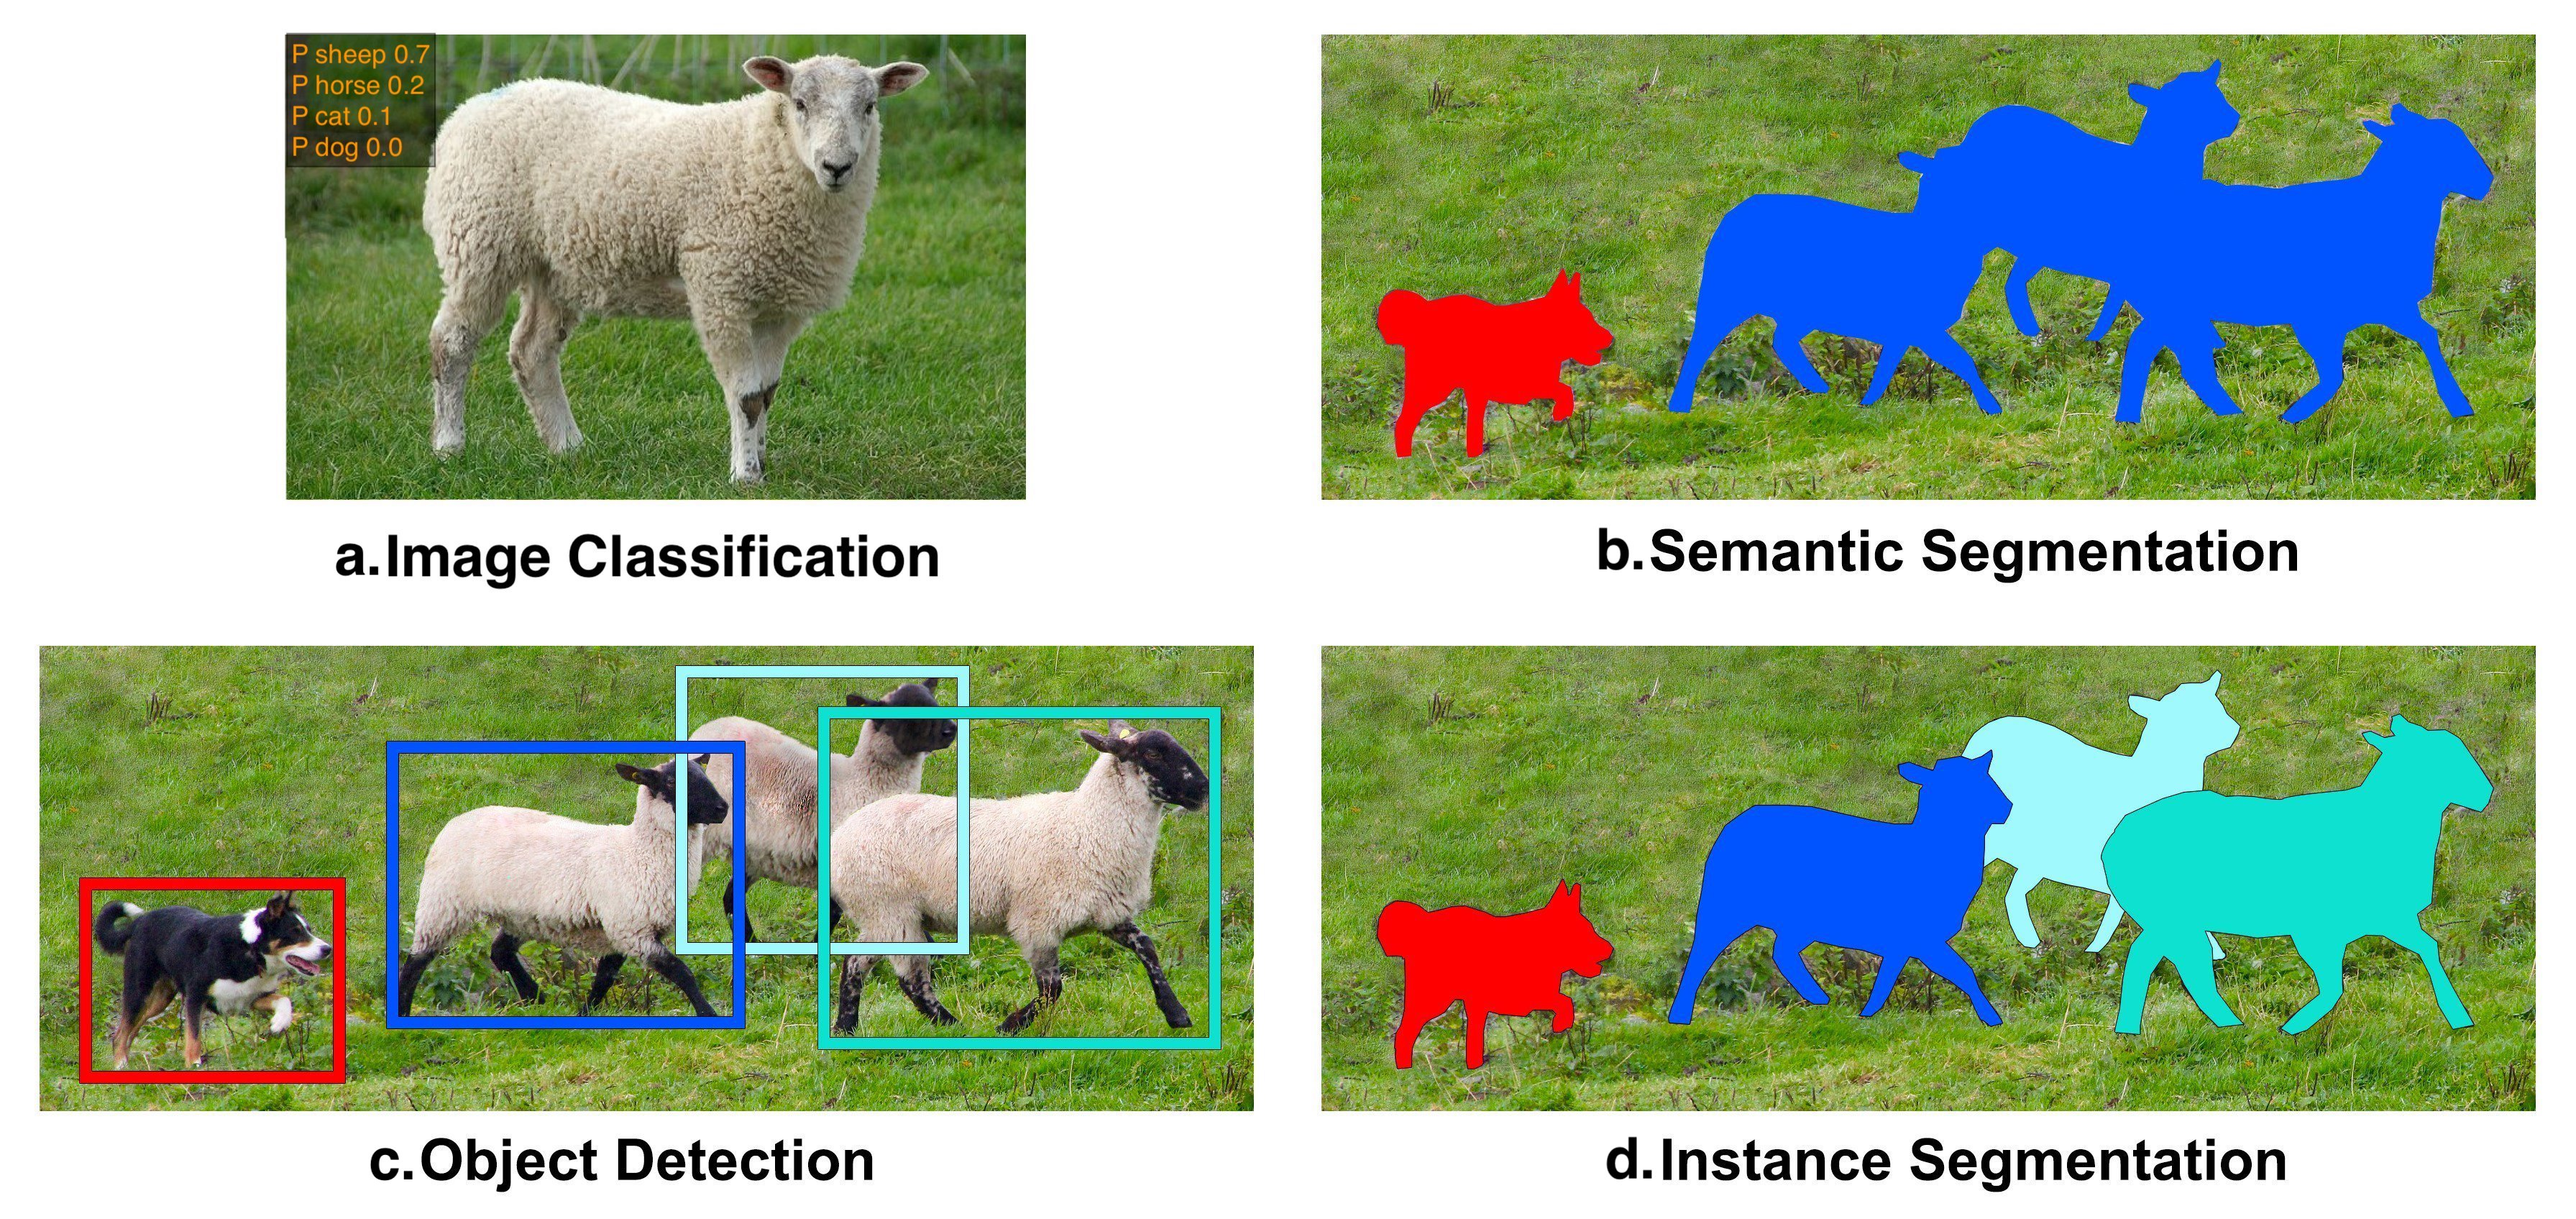
\includegraphics[width=4in]{figures/diff_cv_tasks.jpeg}
    \caption{Different Computer Vision Tasks \cite{diff_detection_segmentation_task_fig}}
    \label{fig:diff_cv_tasks}
\end{figure}

We begin with image classification, the most fundamental task in the computer vision field. The task involves assigning an object category label to an input image, assuming the input image contains exactly one object \cite{overview_cv_task}. This implies that the task allows the object classification label to be given to the entire image without specifying where the object is. As shown in Figure \ref{fig:diff_cv_tasks}a, the image classification model predicts the probability that the image shows a sheep, a horse, a cat, or a dog. Although image classification is comparatively simpler than other computer vision tasks, it presents several significant challenges due to the variability of image appearance caused by changes in scale, orientation, lighting, occlusions, and other factors.

The second task is semantic segmentation. In contrast to image classification, semantic segmentation is unconcerned with the presence or absence of objects in the input image. The objective of the task is to classify each pixel of the input image into one of several predefined classes or categories \cite{overview_cv_task}. By classifying each pixel, the task generates a detailed mapping between image pixels and classes that can be used to locate and outline objects of different classes within the image. However, when classifying each pixel without consideration of object location, the task removes the depth dimension of the image. That is, if two objects of the same class are positioned behind one another, then the semantic segmentation model will consider them as one object of this class, thus losing dimension information. Considering Figure \ref{fig:diff_cv_tasks}b, we noted the three sheep are at different locations in the depth dimension, but the semantic segmentation mask visualizes these sheep as one object in 2-dimensional space.

The third task is object detection, an improvement over image classification. The goal of object detection models is to locate and categorize each object within a given image \cite{overview_cv_task}. The process of object detection involves two main subtasks: object localization and object classification. Object localization determines the location and size of each object in an image by predicting a bounding box around the object. Once the object is localized, it can be classified using an image classification model. Compared to semantic segmentation, object detection retains all spatial information of the object in the image but loses the pixel accuracy mask. This is illustrated in Figures \ref{fig:diff_cv_tasks}c and \ref{fig:diff_cv_tasks}d, where object detection is able to detect all three sheep, but it is unclear whether a pixel within the bounding box refers to the sheep or the grass behind it.

The last task we want to discuss is instance segmentation. For every object in a given image or video frame, the instance segmentation model must identify all pixels belonging to the object and assign a category label to the object \cite{overview_cv_task}. Identifying all pixels that belong to the object creates the object's mask, which may then be used to locate pixel-precise locations and the object's outline. While object detection and instance segmentation involve locating objects, the former offers information about the location and scale of the detected objects, whereas the latter goes further by identifying all pixels associated with the object. On the other hand, the main distinction between instance and semantic segmentation lies in the level of detail they provide. While semantic segmentation divides an image into classes such as "vehicle" or "animal", instance segmentation provides more details by distinguishing between each individual object within those classes. It accomplishes this by assigning each object a unique label for identification. This means that instance segmentation can determine not only the class of each object in an image but also where it is located and how many there are - something semantic segmentation cannot achieve on its own. Considering Figure \ref{fig:diff_cv_tasks}, we observed that instance segmentation creates a pixel-accurate outline of all four animals, in contrast to the bounding box generated by object detection. In addition, the instance segmentation model's pixel-by-pixel mask must differentiate between the three sheep in contrast to semantic segmentation. In other words, the instance segmentation model combines object detection and semantic segmentation strengths while eliminating their weaknesses.
 
R-CNN and YOLO are two popular families of models used for object detection and instance segmentation. In Sections \ref{chap:rcnn_variation} and \ref{chap:yolo_variation}, we will delve into the variations of R-CNN and YOLO model, respectively. However, before we proceed, it is essential to understand the metrics used for assessing the performance of an object detection or instance segmentation model. In the next subsection, we will discuss the metrics utilized for evaluating these models.

\section{Evaluation Metrics}  \label{sec:eval_metrics}

As previously mentioned, an object detection model is responsible for localizing and classifying objects in an image by predicting a bounding box for each object and assigning a class label. Therefore, to evaluate the performance of an object detection model, the accuracy of the predicted bounding box and the given class label must be evaluated. Similarly, while evaluating an instance segmentation model, it is critical to analyze the quality of the pixel-wise mask in addition to the bounding box and category label. As a result, in this section, we will go over the metrics used to assess the accuracy of the bounding box, category label, and pixel-wise mask.

\subsection{Intersection over Union (IoU) Metric}  \label{subsec:iou_metric}
We start by discussing the evaluation metric for bounding box accuracy in the object detection task. In this task, the model predicts a bounding box for each object in the image to describe the object's location and size. The bounding boxes are commonly represented as a tuple $(x_{min},\ y_{min},\ x_{max},\ y_{max})$ indicating the coordinates of the top-left and bottom-right corners of the box. To evaluate the accuracy of the predicted bounding box, we compare its coordinates with the coordinate of a ground-truth bounding box. Each ground-truth bounding box is a manually annotated rectangle that precisely encloses an object in the image or video frame. With the ground-truth boxes, \textbf{Intersection over Union (IoU)}, also known as the Jaccard index or Jaccard similarity coefficient, the metric for measuring the degree of overlap between the predicted bounding box and the ground-truth bounding box for a given object \cite{generalized_iou}. In other words, given two rectangles represent the predicted bounding box and the ground-truth box, then the IoU can be expressed as:
\begin{equation}
    \text{IoU} = \frac{Area(BB_p \cap BB_t)}{Area(BB_p \cup BB_t)} \label{eq:iou}
\end{equation}
where $BB_p$ is the predicted bounding box, and $BB_t$ is the ground-truth bounding box. The IoU metric is defined in the range [0, 1], where a value closer to 0 indicates no overlap between bounding boxes, and 1 indicates a perfect overlap. Since $Area_{rectangle} = height \times width$, by comparing the area of two rectangles, the IoU metric incorporates the size and aspect ratio of the two boxes in comparison. As a result, the IoU metric is invariant to the size and aspect ratio. Due to its simplicity and invariance properties, IoU is widely used to measure the accuracy of predicted bounding boxes in various computer vision tasks \cite{generalized_iou}. Despite its success as a metric, IoU has a major weakness that prevents it from being used as a loss function. As shown in Equation \ref{eq:iou}, we noted that as long as the overlapping area is 0, i.e., $Area(BB_p \cap BB_t) = 0$, then IoU will be 0. In other words, when the predicted and ground-truth bounding boxes are not overlapping, the resulting IoU score does not indicate whether they are near or far from each other. The Generalized Intersection over Union (GIoU) was proposed to resolve this issue, as described in \cite{generalized_iou}.

\subsection{IoU Threshold and Confidence Threshold}  \label{subsec:iou_conf_threshold}
Next, we can assess the model's accuracy in classifying the object within each bounding box. Each bounding box requires the model to predict a categorical label and a confidence score. The label denotes the object's class within the bounding box, and the score reflects the model's confidence in identifying the object as belonging to this class. To assess the model's accuracy, we compare the predicted bounding box label with the ground-truth bounding box label. Before comparing the predicted box and ground-truth box labels, it is crucial to require that the degree of overlap between them meets a certain threshold $t_{IoU}$. If IoU $\geq t_{IoU}$, the detection is considered as a positive sample, whereas if IoU $< t_{IoU}$, the detection is considered as a negative sample. For each positive sample, we check if the model's confidence is higher than a predetermined threshold, $t_{confidence}$. If the confidence score meets the threshold, we compare the predicted label with the ground-truth label. Conversely, the comparison will result in a false if a bounding box is classified as a negative sample or has a confidence score lower than $t_{confidence}$. Therefore, to correctly classify a predicted bounding box, the model must satisfy three conditions: (1) the IoU score $\geq t_{IoU}$, (2) the confidence score $\geq t_{confidence}$, and (3) the predicted label matches the ground-truth label. If any of these conditions are not met, the model has incorrectly classified the predicted box.

The first condition (IoU score $\geq t_{IoU}$) is required because, assuming the second and third conditions are met, if the predicted bounding box and the ground-truth bounding box have little or no overlap, then the prediction should be considered false, and the model's accuracy should be reduced. The value of $t_{IoU}$ depends heavily on the task the model tries to accomplish. For tasks that require absolute precision, such as human surgery assistance, $t_{IoU}$ should be set high. However, a much lower threshold is more forgiving for tasks like checking the presence of a glass of water on the table. For evaluating the overall performance of the model, a $t_{IoU}$ value of 0.5 can be used, as demonstrated in the PASCAL VOC benchmark \cite{pascal_voc_2015}. Alternatively, the model can be evaluated at each $t_{IoU} \in \{0.50, 0.55, ..., 0.95\}$, as shown in the COCO benchmark \cite{coco_2014}. On the other hand, the second condition (confidence score $\geq t_{confidence}$) is necessary because the score directly affects the model's behavior in predicting accurately versus finding all occurrences. This behavior is denoted as the tradeoff between precision and recall, which we will discuss later in this section.

As an example, consider an image with 3 cars and 1 human. After processing the image with our object detection model, 2 cars and 1 human are identified with confidence scores of 0.76, 0.72, and 0.58, and IoU scores of 0.89, 0.32, and 0.52, respectively. The results are shown in the following table:
\begin{table}[H]
    \centering
    \begin{tabular}{rcccc}
        ground-truth labels         & car  & car  & car  & human \\ \hline
        predicted labels            & car  & car  & none & human \\ \hline
        predicted confidence scores & 0.76 & 0.72 & 0    & 0.58  \\ \hline
        predicted IoU scores        & 0.89 & 0.32 & 0    & 0.52 
    \end{tabular}
    \caption{Example's representation: Input image contains 3 cars and 1 human. The model predicts 2 cars and 1 human with respective confidence scores of 0.76, 0.72, and 0.58, and IoU scores of 0.89, 0.32, and 0.52} \label{ex:truth_pred_score_map}
\end{table}

Assuming the confidence threshold $t_{confidence}=0.6$, any predicted bounding box with confidence score lower than 0.2 will be removed. Additionally, assuming the IoU threshold $t_{IoU}=0.5$, then the truth bouding box with IoU score lower than 0.5 will be removed \cite{metrics_survey_2020}. In this example, one of the predicted car is 68\% offset from its truth location, hence the corresponding truth car label being removed. Thus the predicted labels and ground-truth labels are mapped one to one as follows:
\begin{table}[H]
    \centering
    \begin{tabular}{rcccc}
    ground-truth labels         & car  & none & car  & human \\ \hline
    predicted labels            & car  & car  & none & none
    \end{tabular}
\end{table}

\noindent Please note that changes in IoU and confidence thresholds can impact the correspondence between predicted and truth labels. For instance, if the IoU threshold ($t_{IoU}$) is adjusted to 0.7, the model will only recognize the first car as a ground-truth object, while the second car and human object (sample) will not be recognized. Similarly, if the confidence threshold ($t_{confidence}$) is set to 0.8, the model will not be able to detect any object, resulting in all predicted labels being classified as None. Therefore, it can be said that the value of $t_{IoU}$ determines whether a truth label is considered in the comparison, while $t_{confidence}$ determines whether a predicted label is considered in the comparison \cite{metrics_survey_2020}.

\subsection{Confusion Matrix}  \label{subsec:confusion_matrix}
The mapping between the predicted and ground-truth labels offers insight into the model's ability to detect and classify samples at a particular confidence and IoU threshold. We can quantify this insight using a confusion matrix, a 2 x 2 matrix that assesses the object detection model's performance in distinguishing between two categories \cite{confusion_matrix_2017}. Since the confusion matrix assumes that there are only two categories, when multiple categories are in the mapping, each category will have its unique confusion matrix. In other words, for each category, the confusion matrix measures the model's ability to differentiate between samples belonging to this category and those that do not. The confusion matrix comprises four different combinations of predicted and ground-truth labels, as shown:
\begin{table}[H]
    \centering
    \begin{tabular}{cc|cc|}
    \cline{3-4}
                                                        &          & \multicolumn{2}{c|}{Predicted}                                 \\ \cline{3-4} 
                                                        &          & \multicolumn{1}{c|}{Negative}            & Positive            \\ \hline
    \multicolumn{1}{|c|}{\multirow{2}{*}{Ground-Truth}} & Negative & \multicolumn{1}{c|}{True Negative (TN)}  & False Positive (FP) \\ \cline{2-4} 
    \multicolumn{1}{|c|}{}                              & Positive & \multicolumn{1}{c|}{False Negative (FN)} & True Positive (TP)  \\ \hline
    \end{tabular}
\end{table}

The \textbf{true negative (TN)} represents the count of times the model correctly recognizes a sample not belonging to a specific class. On the other hand, the \textbf{false negative (FN)} represents the number of ground-truth samples where the model fails to detect an object of this class at that position. The \textbf{false positive (FP)} is the count of samples that the model identifies as objects of this class at that position where there is no object or the IoU score is low. Lastly, the \textbf{true positive (TP)} denotes the number of ground-truth samples accurately recognized by the model. Consider Example \ref{ex:truth_pred_score_map}. Since we have two classes, we will have a confusion matrix for each class. Take the car class, for example, then:
\begin{itemize}
    \item True negative: The number of times the model \emph{correctly} classifies \emph{a none-car object as not a car}.
    \item False negative: The number of times the model \emph{incorrectly} classifies \emph{a car object as not a car}.
    \item False positive: The number of times the model \emph{incorrectly} classifies \emph{a none-car object as a car} or classifies \emph{a car object as a car but at a wrong location}.
    \item True positive: The number of times the model \emph{correctly} classifies \emph{a car object as a car}.
\end{itemize}
By utilizing these definitions, we can create the confusion matrix for the car class and, similarly, for the human class, with thresholds $t_{IoU}=0.5$ and $t_{confidence}=0.6$ as follow:
\begin{table}[H]
    \centering
    \begin{tabular}{cccc}
        \multicolumn{4}{c}{Confusion Matrix for Car Class} \\ \cline{3-4} 
                                                                                                          & \multicolumn{1}{c|}{}         & \multicolumn{2}{c|}{Predicted}                                \\ \cline{3-4} 
                                                                                                          & \multicolumn{1}{c|}{}         & \multicolumn{1}{c|}{Negative} & \multicolumn{1}{c|}{Positive} \\ \hline
        \multicolumn{1}{|c|}{\multirow{2}{*}{\begin{tabular}[c]{@{}c@{}}Ground\\ Truth\end{tabular}}}     & \multicolumn{1}{c|}{Negative} & \multicolumn{1}{c|}{1}        & \multicolumn{1}{c|}{1}        \\ \cline{2-4} 
        \multicolumn{1}{|c|}{}                                                                            & \multicolumn{1}{c|}{Positive} & \multicolumn{1}{c|}{1}        & \multicolumn{1}{c|}{1}        \\ \hline
    \end{tabular}
    \qquad
    \begin{tabular}{cccc}
        \multicolumn{4}{c}{Confusion Matrix for Human Class}                                                                                                                                              \\ \cline{3-4} 
                                                                                                          & \multicolumn{1}{c|}{}         & \multicolumn{2}{c|}{Predicted}                                \\ \cline{3-4} 
                                                                                                          & \multicolumn{1}{c|}{}         & \multicolumn{1}{c|}{Negative} & \multicolumn{1}{c|}{Positive} \\ \hline
        \multicolumn{1}{|c|}{\multirow{2}{*}{\begin{tabular}[c]{@{}c@{}}Ground\\ Truth\end{tabular}}}     & \multicolumn{1}{c|}{Negative} & \multicolumn{1}{c|}{3}        & \multicolumn{1}{c|}{0}        \\ \cline{2-4} 
        \multicolumn{1}{|c|}{}                                                                            & \multicolumn{1}{c|}{Positive} & \multicolumn{1}{c|}{1}        & \multicolumn{1}{c|}{0}        \\ \hline
    \end{tabular}
\end{table}
\noindent where in the car confusion matrix, FP$=1$ because ground-truth label is "none" while predicted label is "car", FN$=1$ because ground-truth label is "car" while predicted label is "none", and TN$=1$ because both ground-truth and predicted label ("human" and "none", respectively) are not "car".

\subsection{Accuracy Metric}  \label{subsec:accuracy_metric}
With the confusion matrix, we can assess the overall object detection model's performance at a particular threshold by computing the accuracy, precision, and recall metrics. First, the \textbf{accuracy (ACC) metric} describes how the model performs in detecting and classifying samples of all known classes. It is determined by dividing the number of correct detections by the total number of predictions made \cite{szeliski_cv_book}, as follows:
\begin{equation}
    ACC = \frac{TN+TP}{TN+FN+TP+FP} \label{eq:accuracy}
\end{equation}
However, the accuracy (ACC) metric is only meaningful when all classes are equally important and the input data has an approximately equal number of samples belonging to each class. The ACC metric can be misleading when some specific classes dominate the input data. For example, suppose a model processes an image of 495 cars and 5 humans. If the model classifies all 500 detections as cars, then the ACC be $\frac{0+495}{0+0+495+5}=0.99$. This result indicates that the model is 99\% correct in detecting the presence of cars and humans, even though it was unable to detect any humans.

\subsection{Precision Metric}  \label{subsec:precision_metric}
An alternative metric that can be utilized is precision. \textbf{Precision metric} assesses the dependability of the model in identifying a detection as positive for a specific class \cite{metrics_survey_2020}. Unlike ACC, precision assesses the model's reliability in classifying a particular class rather than across all classes. Thus, the precision performance of the model is different for each class at a given threshold. Precision is defined in the range of $[0,1]$  as:
\begin{equation}
    Precision = \frac{TP}{TP+FP} \label{eq:precision}
\end{equation}
A precision score of 0 signifies that all samples identified by the model as belonging to this particular class are incorrect, while a score of 1 indicates that all predictions for this class are accurate. However, precision does not reflect instances where the model fails to identify some samples of this class. Take the car class in Table \ref{ex:truth_pred_score_map} as an example. Let assume the model correctly classify the seconf car as a car at a higher IoU value of 0.8, then the ground-truth and predicted labels correspondence map is:
\begin{table}[H]
    \centering
    \begin{tabular}{rcccc}
    ground-truth labels         & car  & car & car  & human \\ \hline
    predicted labels            & car  & car & none & none
    \end{tabular}
\end{table}
\noindent Therefore, the precision score for this class is $\frac{2}{2+0}=1$, indicating that when the model predicts a sample as a car, the ground-truth label for that sample is indeed a car 100\% of the time. However, it is worth noting that the precision score does not factor in the car that the model missed in our example.

\subsection{Recall Metric}  \label{subsec:recall_metric}
As previously stated, precision only measures the correctness of detections but not the model's ability to detect all samples of a particular class. \textbf{Recall metric} are often utilized in conjunction with precision to overcome this limitation. The recall is mathematically defined in the range of $[0,1]$ as:
\begin{equation}
    Recall = \frac{TP}{TP+FN} \label{eq:recall}
\end{equation}
A value of 0 denotes that the model has missed identifying all ground-truth samples belonging to this class, while a value of 1 indicates that the model has detected all ground-truth samples of this class \cite{metrics_survey_2020}. However, similar to other metrics, recall is not flawless, as it does not account for instances where the model classifies all negative samples as belonging to this class. For instance, consider the car class in Table \ref{ex:truth_pred_score_map}. If our model predicts all ground-truth samples as belonging to the car class, the car class's recall is $\frac{3}{3+0}=1$, suggesting that the model can identify all ground-truth cars. However, as illustrated, the recall value fails to account for the model's misclassification of a non-car (human) object as a car. This error can be detected by the false positive (FP) term in the precision metric. Therefore, precision and recall are typically used together to evaluate an object detection model.

Using the definition of precision and recall, we noted that the two metrics measure the model's accuracy in classifying objects of a particular class at a particular confidence threshold $t_{confidence}$. We denote objects belonging to this class referred to as positive samples, while those that do not belong are negative samples. Based on Equation \ref{eq:precision}, we can see that as the precision approaches 1, the true positive (TP) term increase while the false positive (FP) term decrease. This implies that the model becomes more confident in classifying a sample as positive as precision increases. On the other hand, Equation \ref{eq:recall} shows that as the true positive (TP) term increases and the false negative (FN) term decreases, the recall approaches 1. This indicates that a higher recall value means the model identifies more samples as positive. 

\subsection{Precision-Recall Curve}  \label{subsec:pr_curve}
As it might be seen, there is a tradeoff between precision and recall. Suppose we establish a high $t_{confidence}$ value for the model and only classify a sample as positive when its confidence score surpasses this threshold. In this case, the model may miss multiple ground-truth positive samples, resulting in high precision but low recall. Conversely, suppose we set a low $t_{confidence}$ value; then, the model may classify most samples as positive, even those that are incorrectly classified, resulting in the model having low precision but high recall. Nonetheless, an object detector is deemed as high performance at a particular IoU threshold if its precision remains high as its recall increases \cite{metrics_survey_2020}. Since the model's precision and recall vary depending on the confidence threshold $t_{confidence}$, we can calculate both metrics for each threshold value to examine the tradeoff between optimizing for one over the other. These computed metric values can be plotted on a two-dimensional plane to visualize the tradeoff, also known as the \textbf{precision-recall curve}. Figure \ref{fig:precision-recall_curve} shows examples of the precision-recall curve for a dataset and how the curve change at different IoU threshold value.

\begin{figure}[!ht]
    \centering
    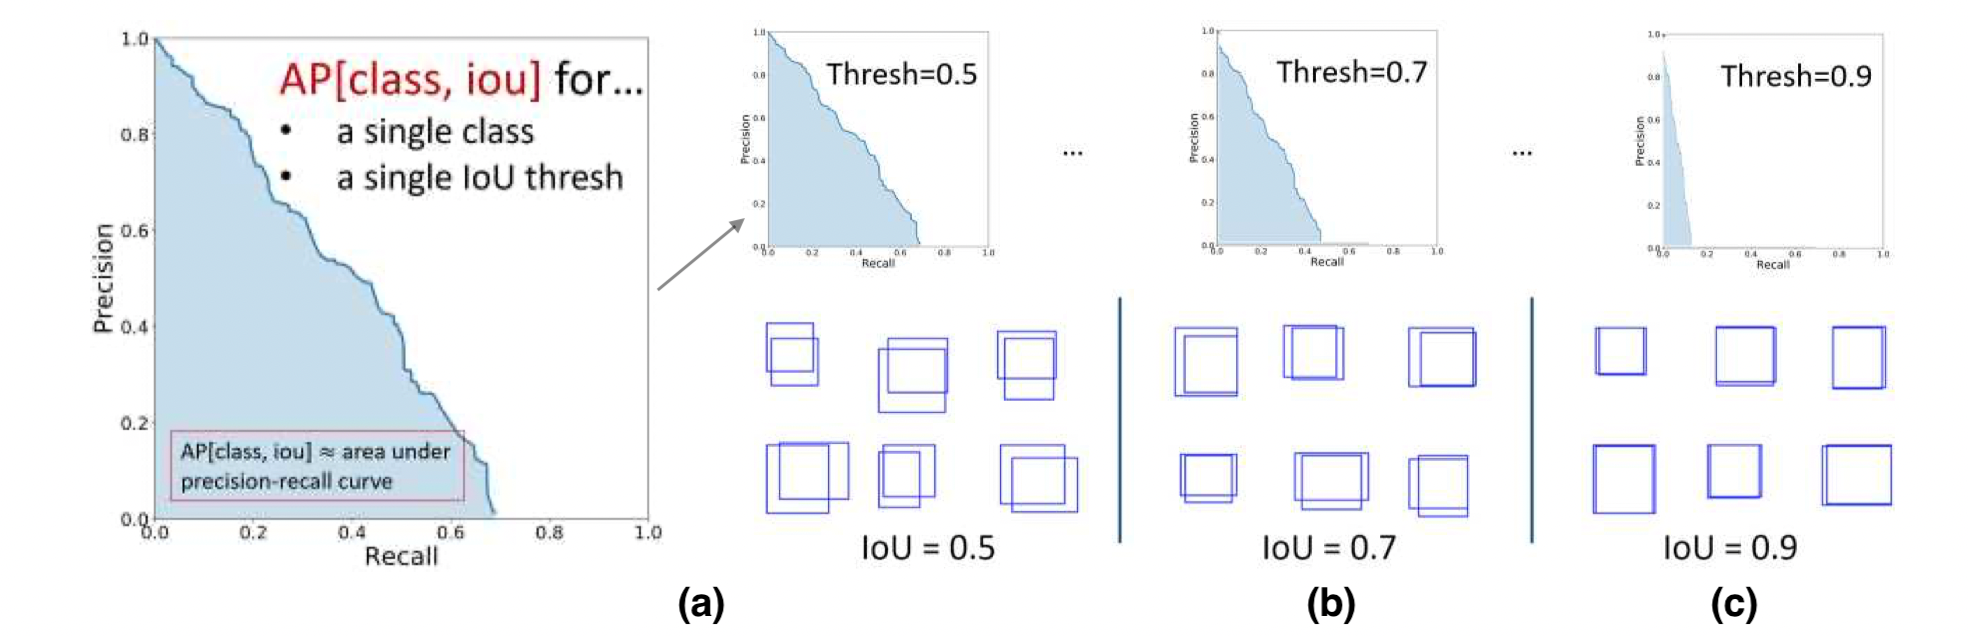
\includegraphics[width=5.5in]{figures/precision_recall_curve.png}
    \caption{\textbf{(a)} The precision-recall curve for a single class at the IoU threshold of 0.5 for a dataset. \textbf{(b, c)} the same precision-recall curve as (a) but with IoU threshold of 0.7 and 0.9, respectively. \cite{szeliski_cv_book}} 
    \label{fig:precision-recall_curve}
\end{figure}

\subsection{F-score (F1-score) Metric}  \label{subsec:f_score}
Optimizing a model for precision or recall, similar to choosing an IoU threshold value, heavily depends on the task the model tries to complete. If the model is used for a high-accuracy and detailed task, such as surgery, it should be optimized for precision metrics. On the other hand, if the task is more focused on catching as many instances as possible, such as low-cost home-based cancer diagnosis, the model should be optimized for recall. In cases where both precision and recall are equally important, we can determine the optimal combination of the two metrics by comparing their F-scores at different confidence thresholds. The F-score is the harmonic mean, a type of numerical average, of the precision and recall metrics \cite{fscore_2017}. For each pair of precision and recall, the F-score can be calculated as follows:
\begin{equation}
    \text{F-score} = 2 \times \frac{Precision \times Recall}{Precision + Recall}
\end{equation}
Given that the F-score is the harmonic mean of precision and recall metrics for a specific class at a confidence threshold $t_{confidence}$, comparing the F-score at different $t_{confidence}$ value help determine the optimal combination of precision and recall. The highest F-score obtained represents this optimal combination, allowing us to select the ideal confidence threshold value.

\subsection{Average Precision (AP) Metric}  \label{subsec:ap_metric}
Another metric that can be used to evaluate the performance of a model for each class is the average precision (AP). While the F-score describes the confidence threshold value at which the model achieves the highest performance for a particular class, the average precision (AP) summarizes the model's performance across various confidence thresholds for that class. In other words, the AP condenses the precision-recall curve for a specific class into a single value representing the average of all precisions. The AP is an estimate of the area under the precision-recall curve. There are different versions of AP; the adopted version for PASCAL VOC and COCO benchmark is the N-point interpolation AP \cite{n_point_interpolation_ap}. Let $P$ and $R$ denote precision and recall, respectively. The N-point interpolation AP is defined as follows:
\begin{equation}
    AP_N = \frac{1}{N} \sum_{R \in \mathbb{R}_N} P_{interp}(R) \qquad with \qquad P_{interp}(R) = \max_{{R}':{R}' \geq R} P({R}')
\end{equation}
where the set of $N$ interpolation $\mathbb{R}_N$ is $\left\{0, \frac{1}{N}, \frac{2}{N}, ..., \frac{N}{N}\right\}$. The term $P({R}')$ is the value of precision at recall ${R}'$. The condition $\max_{{R}':{R}' \geq R}$ implies that the $P_{interp}(R)$ is the highest precision value among all recall point ${R}'$ that are larger than $R$, instead of being the precision observed at the recall $R$ \cite{n_point_interpolation_ap}. As an example, consider using 11-point interpolation to the precision-recall curve shown in Figure \ref{fig:11AP_ex}. With this precision-recall curve, the 11-point interpolation AP is:
\begin{equation*}
    AP_{11} = \frac{1}{11} (1+0.666+3 \times 0.428 + 6 \times 0) \approx 26.818\% 
\end{equation*}
We noted that instead of using the precision value at each recall in $\left\{0, \frac{1}{10}, \frac{2}{10}, ..., \frac{10}{10}\right\}$, the $AP_{11}$ use the maximum precision value of all the remaining recall points. While the N-point interpolation technique simplifies the computation of the average precision (AP), it is an approximation method that yields a non-differentiable AP value. The difficulties in optimizing non-differentiable values make it challenging to use AP as a loss function. To address this limitation, recent research has proposed metrics like probability-based detection quality (PDQ) and Smooth-AP \cite{pdq_metric_2020, smoth_ap_metric_2020}.

\begin{figure}[!ht]
    \centering
    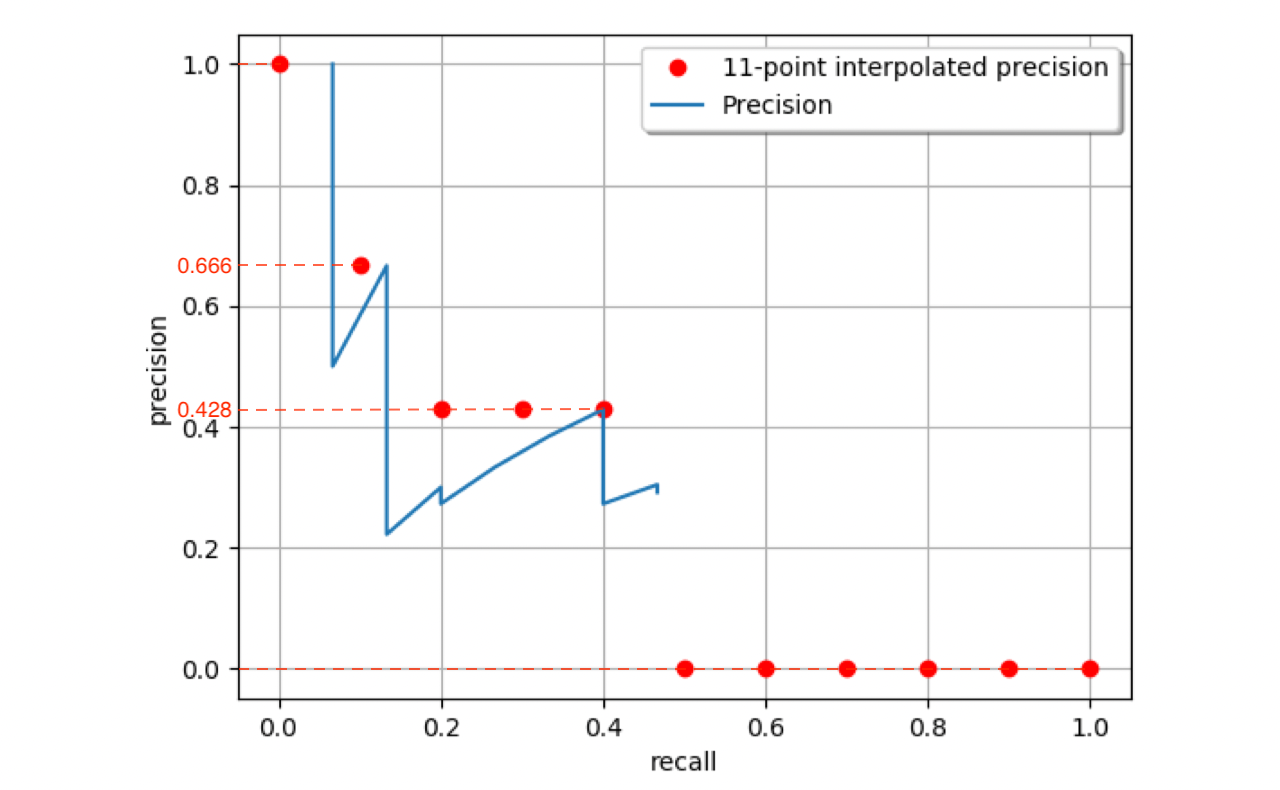
\includegraphics[width=4in]{figures/11AP_ex.png}
    \caption{Applied 11-point interpolation method on the precision-recall curve \cite{metrics_survey_2020}}
    \label{fig:11AP_ex}
\end{figure}

\subsection{Mean Average Precision (mAP) Metric}  \label{subsec:mean_ap_metric}
The mean average precision (mAP) of a class can be calculated using the average precision (AP) for that class at a specified IoU threshold \cite{szeliski_cv_book}. The mAP quantifies the model's accuracy in detecting objects of all classes above a particular IoU threshold. Let $K$ be the number of classes our model able to predict object for, then mAP is defined as follows:
\begin{equation}
    mAP = \frac{1}{K} \sum_{i=1}^{i=K}AP_i
\end{equation}
where $AP_i$ is the average precision value of the $i$th class.

In summary, evaluating object detection models is a five-step process. First, the Intersection over Union (IoU) between the predicted and ground-truth bounding boxes is calculated to determine the detection's location correctness. Second, a confusion matrix is created by comparing the predicted labels against the ground-truth labels at each IoU and confidence threshold. Third, the model's reliability and sensitivity can be quantified from the confusion matrix at each combination of the two thresholds by computing the precision and recall metrics. Moreover, the precision-recall curve and F-score can be computed to offer insights into the balance between the model's reliability and sensitivity. Fourth, the average precision (AP) metric is calculated to quantify the model's accuracy in detecting objects of a specific class at each IoU threshold. Finally, the mean average precision (mAP) metric represents the model's accuracy in detecting objects across all classes at a given IoU threshold. 

In comparison to object detection, instance segmentation models provide a more detailed output by generating a pixel-wise mask of the object, along with the object's bounding box and classification label. Therefore, to fully assess the performance of an instance segmentation model, we need to evaluate the accuracy of the detection at the pixel level. Similar to the bounding box, the accuracy of the object's mask can be measured using the Intersection over Union (IoU) metric, denoted as \emph{mask IoU} \cite{instance_segementation_metric_2022, mask_rcnn_2017}. The IoU for the object's mask is the ratio of overlapping pixels in the predicted and ground-truth masks over the total number of pixels in both. Consider representing the masks' bounding box as matrices, denoting a value of 1 to the pixels belonging to the object (i.e., inside the mask) and 0 to the pixels not (i.e., outside the mask). The union of the two mask matrices is the number of 1s in either matrix. The intersection is the number of 1s present in the output matrix of the element-wise product (Hadamard product) between the two masks' matrices. After computing the IoU for each pair of object masks, the subsequent steps for evaluating the model are identical to those used for object detection. This entails calculating the confusion matrix, precision-recall curve, F-score, AP, and mAP, but utilizing the mask's IoU rather than the bounding box's IoU.

With the understanding of object detection, instance segmentation, and their evaluation metrics, we will discuss R-CNN and YOLO, the two most popular algorithm families in these tasks, in Chapters \ref{chap:rcnn_variation} and \ref{chap:yolo_variation}, respectively. In Section \ref{sec:cnn}, we discussed the structure and building blocks of convolutional neural networks (CNNs). We also stated how CNNs classify objects in the image classification task in the discussion. However,  the image classification task assumes the image has exactly one object, and the model classifies the entire image based on that one object. Therefore, if we consider each bounding box as its own image, we can utilize a CNN to identify the object's class within the bounding box. This is the main idea behind the different variations of R-CNN and YOLO, which are designed for object detection and instance segmentation task. 
%!TEX root = ../username.tex
\chapter{R-CNN Variation} \label{chap:rcnn_variation}

Since the interested domain for this paper is the instance segmentation task,
we will analyze the Mask R-CNN. Mask R-CNN is a popular algorithm that tries to
solve instance segmentation problem in the Computer Vision field. However, Mask
R-CNN is the improved version of Faster R-CNN and Fast R-CNN, which is based on
the R-CNN algorithm. Therefore, to fully understand Mask R-CNN, we will start
with understanding the building block of R-CNN, which is an object detection
algorithm.

\section{R-CNN}

R-CNN, also known as regional-based convolutional neural networks, is an object detection algorithm. The algorithm was developed by a group of researchers at UC Berkeley in 2015. Since its development, the R-CNN model has revolutionized the field of computer vision. The model was designed to detect up to 80 different types of objects in images and provide large-scale object recognition capabilities. Additionally, before the existence of RCNN, most algorithms in object recognition task used support vector machine (SVM) with blockwise orientation histograms like Histogram of Oriented Gradients (HOG) \cite{svm_hog} or Scale-Invariant Feature Transform (SIFT) \cite{svm_sift}. SVM dominated the space until 2012. In 2012, a CNN algorithm showed an astounding image classification accuracy on ImageNet Large Scale Visual Recognition Challenge (ILSVRC). Since then, more studies have been created into developing and improving algorithms utilizing CNN. The R-CNN model is our first attempt to build an object detection model that extracts features using a pre-trained CNN.

\begin{figure}[!ht]
    \centering
    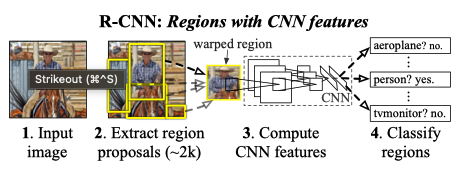
\includegraphics[width=4.5in]{figures/rcnn_archiet.png}
    \caption{R-CNN overall architecture \cite{Girshick_R_CNN_2013}} \label{fig:rcnn_archiet}
\end{figure}

In a board picture, the R-CNN model is composed of three modules [Fig. \ref{fig:rcnn_archiet}]. The first module's purpose is to generate regions of interest (RoI), i.e., regions that possibly contain an object. The second module utilizes a CNN to extract out feature vector from each proposed region. The third module then performs classification for each region using a pre-trained SVM algorithm on the feature vectors provided by the second module. As we can see R-CNN algorithm tries to find the location of each object, extract the object features, and classify these features. Next, we will dive deeper into each module of R-CNN.

\subsection{The First Module: Region Proposal}
In the first module, the algorithm used in this step must be able to propose some region of interest (RoI). A region of interest is a smaller part of the original image that could contain an object.

Given this problem, one might consider the bruce-force method by examining every small rectangle area of the original image as a potential region of interest in a systematic way. This method is the main concept behind the sliding-window technique, a type of exhaustive search algorithm used in the region proposal task. The sliding window technique involves running a window of a predefined size across the image, such that each subsection of the image is considered as a potential region proposal. Like the CNN kernel, the windows' size, stride, and padding are all customizable and can be adjusted to suit different types of images. In addition, multiple scales can also be incorporated into the sliding window technique, which allows for more robust performance in scenarios where objects may appear at different sizes within the same image. Since the sliding window technique examines every location within the image by considering every pixel as part of some RoI, it will not miss any potential object location. However, considering every location in the image as an RoI is unnecessary due to objects most likely not appearing everywhere in the image. Furthermore, classifying every sub-image at different sizes will require tremendous computational power. Therefore, even though it allows our model to detect all possible locations, the sliding window technique should not be used in autonomous cars' vision because it is computationally expensive.

In recent years, many studies have shown interest in improving the efficiency of the region proposal algorithm. One notable algorithm that gives the same strength as the sliding window technique is selective search. The selective search was designed to combine the strength of both exhaustive search and segmentation \cite{selective_search_2013}. The strength that selective search inherits from sliding windows is the ability to find all the possible locations that can be a potential region of interest. Additionally, selective search utilizes the underlying image structure to cluster pixels into different regions, taken from the strength of the segmentation technique. Selective search also aims to complete three goals. These three goals are to capture all scales, diversification, and fast to compute. Capture all scale is the idea that the algorithm must be able to detect objects of different sizes in the image. Next, diversification requirements refer to a method of grouping regions. The algorithm must be able to combine regions containing part of an object into one region. Additionally, for instance, like a person inside a car or a person in front of a car, the algorithm must be able to separate the region for the car and the region for the person under diversification requirement. Lastly, fast computing requires the algorithm not to demand heavy computational power.

As for selective search overall behavior, it can be thought of as two steps. The first step is to perform \textbf{bottom-up segmentation} -- described in Efficient Graph-Based Image Segmentation by Felzenszwalb and Huttenlocher \cite{felzenszwalb_huttenlocher_2004} -- to generate initial sub-segmentation. The second step is to combine similar sub-segmentation recursive using a similarity score between subsegments. The similarity score is a combination of four similarity grouping criteria. These four criteria are color similarity, texture similarity, size similarity, and fill similarity \cite{selective_search_2013}. The reason that color and texture similarity between regions is needed is that the same object most likely will have the same texture or shade of color. In the original paper, the color and texture similarity criteria score can be described by an equation only based on a fixed number of values taken from the histogram of each color channel. Thus, these two similarity scores require minimal to no computational power to compute. Similarly, two regions that have the majority of the area overlap with each other are most likely described the same object. Therefore, the use of a fill similarity score allows the algorithm to merge regions that mostly overlap and keep regions that are not overlapping separate from each other. The fill similarity score can be calculated using the following equation: 
%
\begin{equation*}
    S_{fill}(r_i, r_j) = 1-\frac{size(BB_{ij})-size(r_i)-size(r_j)}{size(image)}
\end{equation*}
%
where $r_i, r_j$ are two considering RoI, and $BB_{ij}$ is the bounding box around $i$ and $j$. Lastly, the similarity in size between the two regions takes into consideration to make sure that the algorithm identifies all locations for different objects at different scales. The size similarity score can be calculated using the following equation: 
%
\begin{equation*}
    S_{size}(r_i, r_j) = 1-\frac{size(r_i)+size(r_j)}{size(image)}
\end{equation*}
%
where $r_i, r_j$ are two considering RoI. As we can see, the similarity score computation is fast and take into account the diversification of the image data set. With these two steps, the selective search can quickly classify foreground and background, then downsample the number of potential RoI that existed in foreground segmentation. Therefore, utilizing selective search allow the model to reduce the number of falsified RoI compared to sliding window and requires lower computational power.

In the original paper of R-CNN, in the first module -- region proposal -- utilize selective search algorithm \cite{Girshick_R_CNN_2013}. However, as mentioned before, the R-CNN model can be thought of as three separate modules; thus, one can experiment with R-CNN with different region proposal techniques.

\subsection{The Second Module: Feature Extraction With CNN}
On completion of the first module of R-CNN, which generates all regions of interest within an image, these RoIs are passed to the AlexNet architect for feature extraction \cite{Girshick_R_CNN_2013}. AlexNet, a CNN architect, was proposed by Alex Krizhevsky at the University of Toronto in 2012 with the guidance of Ilya Sutskever and Geoffrey E. Hinton \cite{AlexNet_2017}. AlexNet was trained using ImageNet, which at the time was the most extensive picture data collection. As AlexNet required its input to have a fixed resolution with the same width and height, the photos in ImageNet were resized to $256 \times 256$ pixels. Prior to publication, AlexNet competed in ILSVRC-2010 and obtained top-one error rates of 37.5\%. In other words, 37.5\% of the time, the model assigns the highest score to the correct label. In the same competition, AlexNet also achieves top-5 error rates of 17.0\%, i.e., the correct label in the top 5 predicts 17\% of the time.

\begin{figure}[!ht]
    \centering
    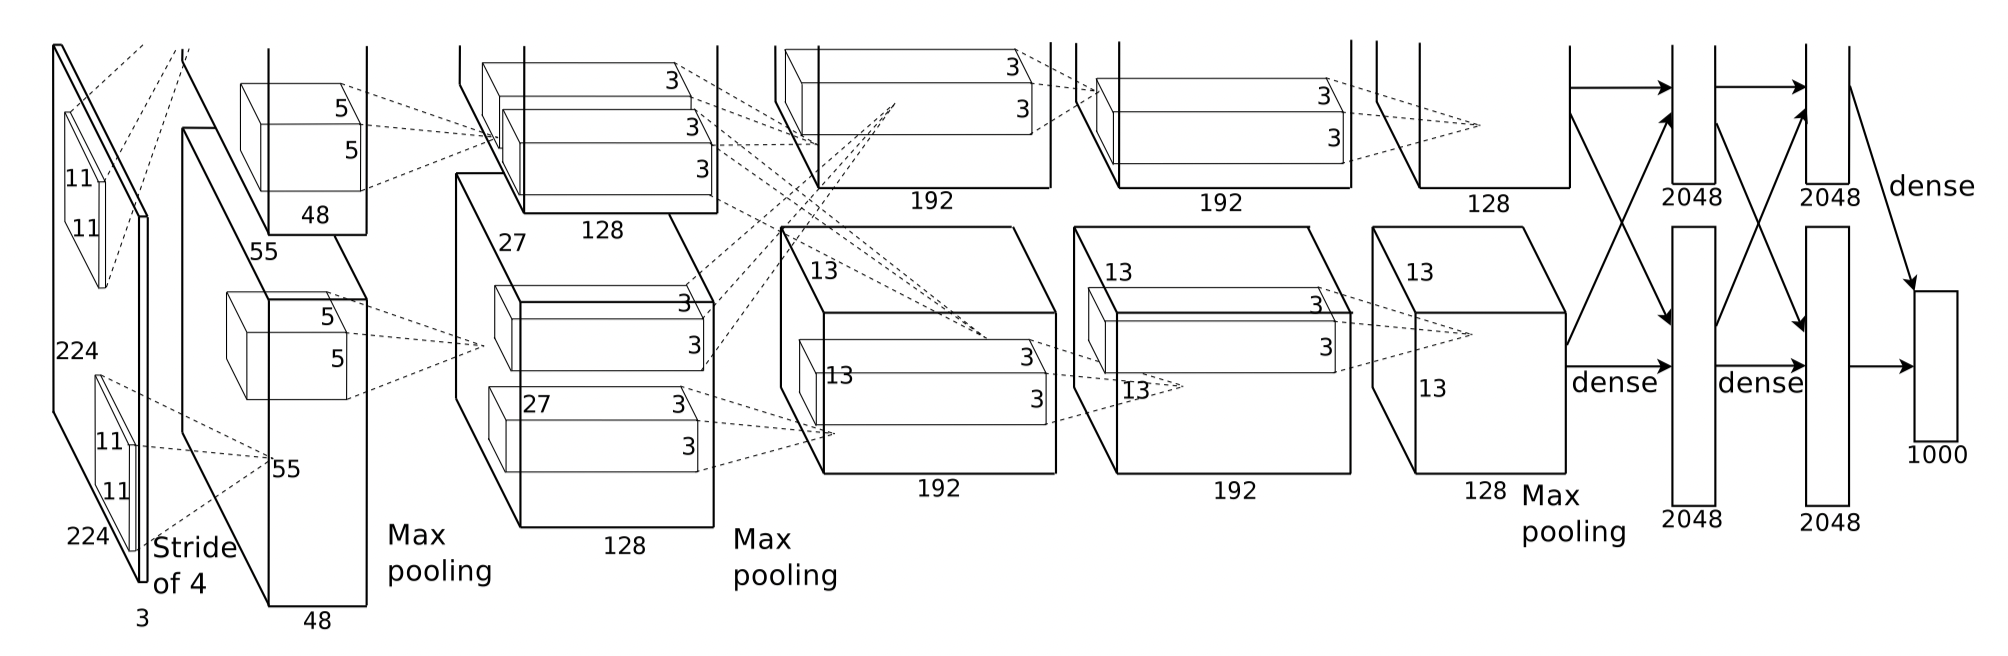
\includegraphics[width=6in]{figures/alex_net.png}
    \caption{AlexNet's overall architecture \cite{AlexNet_2017}} \label{fig:alex_net_architecture}
\end{figure}

AlexNet is regarded as one of CNN's most significant innovations. AlexNet, with 60 million parameters and 650,000 neurons as of 2012, is one of the largest neural networks ever suggested. The architecture of AlexNet consists of eight learned layers. Five convolutional layers are followed by three layers that are fully connected. Due to hardware limitations at the time, it was not possible to fit a massive network like AlexNet on a single GPU. For this reason, the model's architecture is distributed across two separate GPUs, and training must pass via both GPUs. Due to this limitation, for each layer in the network, the model has half of the neurons for that layer on each GPU and only requires particular layers to perform GPU communication. For example, in the overall architecture of AlexNet presented in Figure \ref{fig:alex_net_architecture}, we note that neurons of the first layer only connect to neurons of the second layer on the same GPU. On the contrary, we notice that all neurons of the second layer are fully connected with neurons in the third layer. The notion of spreading neurons across multiple GPUs is known as the parallelization scheme. The parallelization scheme is a topic that remains outside the scope of this paper, and GPU memory size is no longer a significant problem due to the current advancement of technology. Therefore, understanding the parallelization scheme is likely to be optional for the analysis of a CNN model.

In addition to being one of the largest networks and employing a parallelization strategy, AlexNet was among the first neural networks to employ ReLUs. The ReLUs activation function was employed instead of the more common $Tanh$ and $Sigmoid$ functions at the time because AlexNet was designed to reduce learning time. Using ReLUs, the model has a faster learning rate, which, according to the author, would vastly increase the performance of large models with a large data set. In addition, AlexNet implements local response normalization (LRN) to assist ReLUs in generalization. The non-trainable LRN layer is utilized following the first and second network layers. Following the first, second, and fifth layers, AlexNet employs a max-pooling layer with a size of 3 and a stride of two 2. The author notes that having an overlapping pooling layer — i.e., size 3 > stride 2 — decreases overfitting in general \cite{AlexNet_2017}.

AlexNet employs data augmentation and dropout techniques to address the issue of overfitting when training an extensive network with a large data set. For data augmentation, AlexNet randomly selects images into batches and resizes them to a resolution of $224 \times 224$. It then generates a copy with horizontal reflection image transformation and a copy with modified intensity for the three RGB channels. The CPU generates these transformed images while the GPU trains on the previous batch, allowing the data augmentation process to be done without incurring any additional performance costs. In addition to data augmentation, AlexNet also uses the dropout technique. If the output of any hidden neurons is less than or equal to 0.5, the network sets its output to 0. This technique reduces the computation required because neurons with 0 need not be considered in the rest of the forward pass or updated during backpropagation. This method also permits neurons in the network to be independent of one another, as no neurons are guaranteed to persist with each training sample.

R-CNN model utilizes the AlexNet architect implemented on the Caffe framework. R-CNN model passes each generated RoI as a separate image to AlexNet for feature extraction. Since the RoI role is to find each object location in the image, thus AlexNet can assume each RoI only have exactly one object. AlexNet also requires image input of fixed resolution $224 \times 224$; thus, R-CNN transform to the required size by warping all pixels in a bounding box of $227 \times 227$.

\subsection{The Third Module: Classification With Pre-trained SVM}

\begin{figure}[!ht]
    \centering
    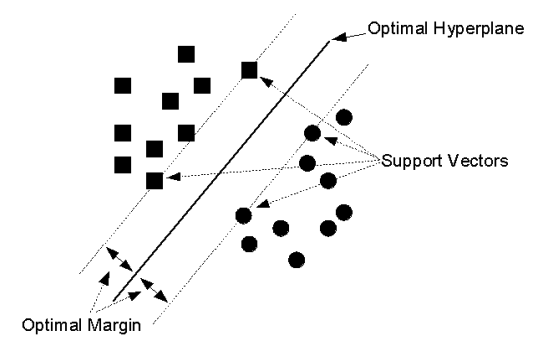
\includegraphics[height=2in]{figures/2d_svm.png}
    \caption{2D linear SVM visualization \cite{2d_svm_Tzotsos}} \label{fig:2d_svm_viz}
\end{figure}

After the second module, R-CNN is able to obtain multiple features for each RoI. Each RoI with extracted features then be given to each trained linear SVM classifier in each class for evaluation. Since each class has its own SVM classifier, thus the SVM only needs to distinguish between objects belonging to the class and objects that are not belonging to the class. Linear SVM classifier can be thought of as trying to draw a $N-1$ dimension separator in the $N$-dimension space where $N$ is the number of features of a specific class. The separator in SVM must be linear, and it tries to separate objects in the class and objects outside of the class. The best-fit separator has the highest margin between any point in the class and any point outside of the class. An example of 2-dimensional linear SVM is visualized by figure \ref{fig:2d_svm_viz} where the circle represents the object in this class, and the square is the object outside the class. Given that the class-specific SVM know what features the class possesses. The separation between objects in and out of the class can be done with little computation power, as we already have the extracted features. Each class SVM is then given the RoI a score representing the likelihood that the object in RoI belongs to this class. Therefore, for each RoI, the class with the highest SVM score is assigned to be the class for the object.

\subsection{R-CNN Result and Drawback}
On the PASCAL VOC dataset 2012, by combining these three modules, R-CNN achieved 53.3\% in \textbf{mean Average Precision (mAP)}. R-CNN also achieves the mAP of 31,4\% and ranks first on the ILSVRC2013 dataset in terms of accuracy \cite{Girshick_R_CNN_2013}. Despite achieving an incredible breakthrough in using Convolutional Networks and having a high object detection accuracy, R-CNN's performance is marred by a number of disadvantages. These issues include multi-stage training, high runtime and space complexity, reliance on non-learnable algorithms, and slowness \cite{fast_rcnn_og}. 

As described by the architecture of R-CNN, the network is divided into three modules and runs sequentially. The network attempts to feed the input of one module with the module's output coming before it. In other words, the first module must completely process the image before the second module is running. Therefore, the network's modules must wait on one another and be trained individually, thus creating the multi-stage training problem. Secondly, since the first module generates 2000 proposed RoIs before the second module can start running, the networks must cache these proposed RoIs on the disk. Similarly, the generated feature for each RoI must be stored on the disk before processing by SVM. The need to write and read multiple time for each RoI cause a high order of runtime and space complexity. The runtime and space complexity is even higher when we consider overlapping RoIs; the network recalculates features and classification for the overlapping portion of overlapping RoIs. Thirdly, the selective search algorithm used in the first module is a non-learnable algorithm. Therefore, the algorithm runtime and accuracy would not improve through training the network. Additionally, through the error analysis, the author notices the mass amount of localization inaccuracy. Thus, for each proposed region, after being scored by the SVMs, the region is piped to a class-specific bounding-box regressor to generate a new bounding box. Finding the bounding box within the region of interest allows the model to improve localization accuracy but exacerbates the model runtime performance as it generates the bounding box at least twice for each object in the image. Lastly, with a processing speed of 47s per image, the R-CNN model is slow and thus has limited real-world application.

\section{Fast R-CNN} \label{sec:fast_rcnn}

The author of R-CNN later implemented Fast R-CNN to reduce the runtime and space complexity while improving detection accuracy. Fast R-CNN is implemented in Python and C++. Like the R-CNN model, Fast R-CNN can be used along with any convolutional neural network. In the proposal Fast R-CNN model, the author utilized VGG16, a one of the deepest CNN in 2015, as the backbone CNN for the model. Comparing the performance of Fast R-CNN with VGG16 versus R-CNN with VGG16 on the PASCAL VOC 2012 dataset, while having the same setup, the experiment showed that Fast R-CNN is 9 times faster at train-time and 213 times faster at test-time while achieving a higher mAP score \cite{fast_rcnn_og}. In the next section, we will mention the keynote of VGG16 architecture, follow by the discussion of Fast R-CNN model and its design decisions that lead to a higher mAP.

\begin{figure}[!ht]
    \centering
    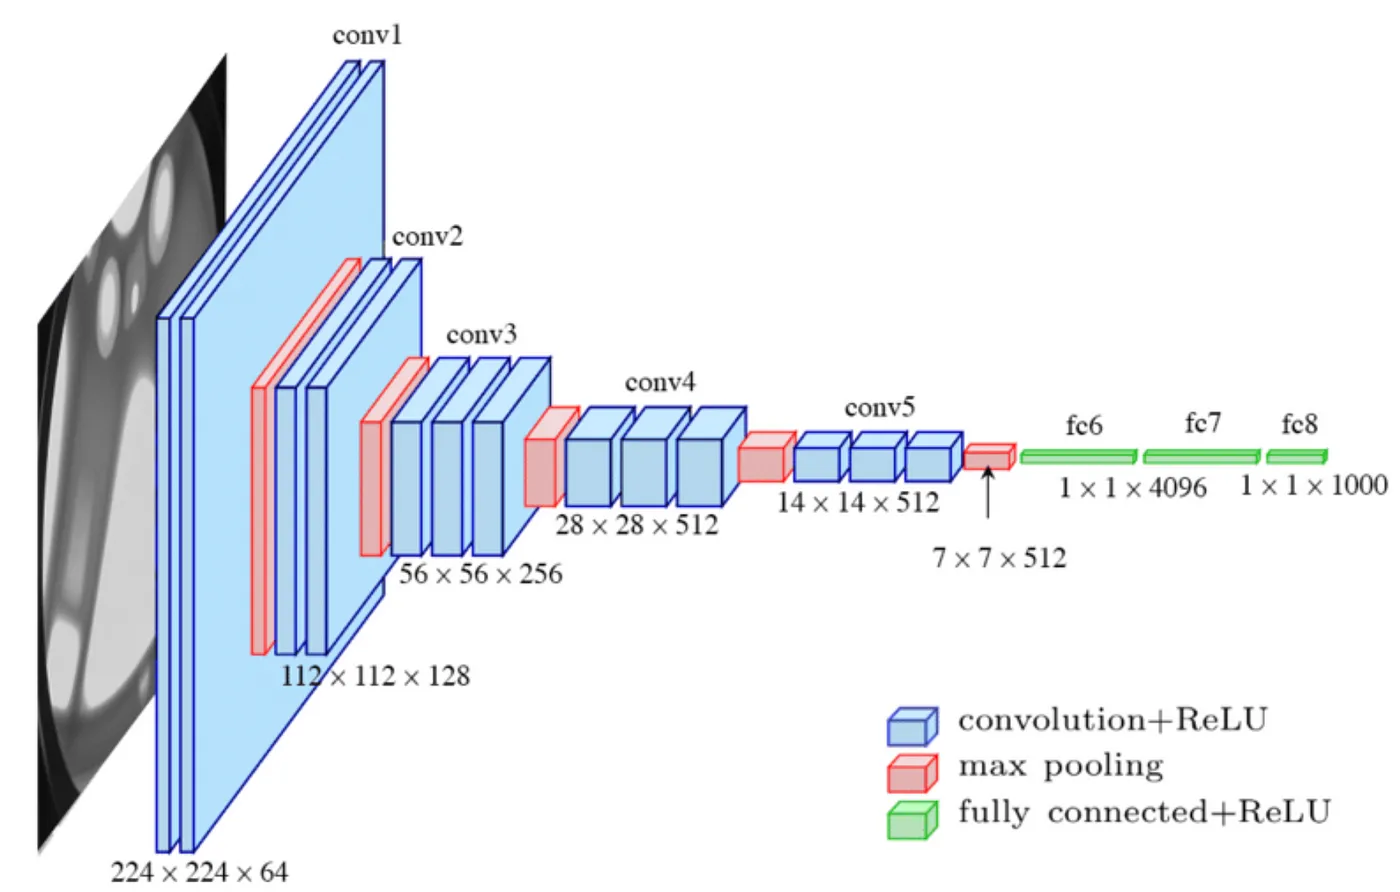
\includegraphics[width=4in]{figures/vgg16_architect.png}
    \caption{VGG16 architecture \cite{vgg16_architect_2014}}
    \label{fig:vgg16_archite}
\end{figure}

The VGG16 is a CNN model developed by the Visual Geometry Group (VGG) at the University of Oxford in 2014 \cite{vgg16_2014}. The VGG16 architecture is notably deeper than AlexNet, comprising 16 learnable layers -- 13 convolutional layers and 3 fully connected layers -- and 5 non-trainable max-pooling layers [Fig. \ref{fig:vgg16_archite}]. VGG16 takes an RGB $224 \times 224$ image as input and generates a $7 \times 7$ feature map, downsampled by a factor of 32 from the input image resolution \cite{deconv_rcnn_2018}. A set of fully connected layers is then processed this feature map to produce the predicted classification label for the image. Unlike AlexNet, which uses a combination of $3 \times 3$ and $5 \times 5$ filters, VGG16 uses only $3 \times 3$ filters throughout the network with smaller strides and padding. By employing a strategy like utilizing a pair of stacked $3 \times 3$ layers in place of a single $5 \times 5$ layer, VGG16's design enabled it to demonstrate that elevating the depth of a network to 16 layers can yield substantial improvements for existing CNNs. Fast R-CNN adapts any CNN model for object detection by performing three changes. The first change is replacing the last pooling layer with an RoI pooling layer (named RoIPool). For VGG16, an RoI will be used in place of the $7 \times 7 \times 512$ max-pool layer in Fast R-CNN. The second change is replacing the last fully connected layer with two sibling layers, i.e., replacing the fc8 layer for VGG16. Lastly, Fast R-CNN will adjust the input layer of the CNN model to accept images of any size and proposed RoIs for that particular image as input. We will discuss these changes in more detail later in this section.

\begin{figure}[!ht]
    \centering
    \subfloat[][Overall architecture \cite{fast_rcnn_og}]{ 
        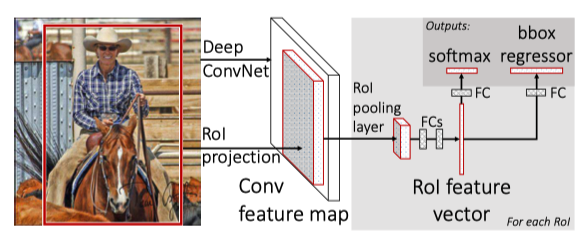
\includegraphics[width=3in]{figures/fast_rcnn_archiet.png} \label{fig:fast_rcnn_archite} 
    }

    \subfloat[][Network flow \cite{rcnn_vari_flow_chart}]{ 
        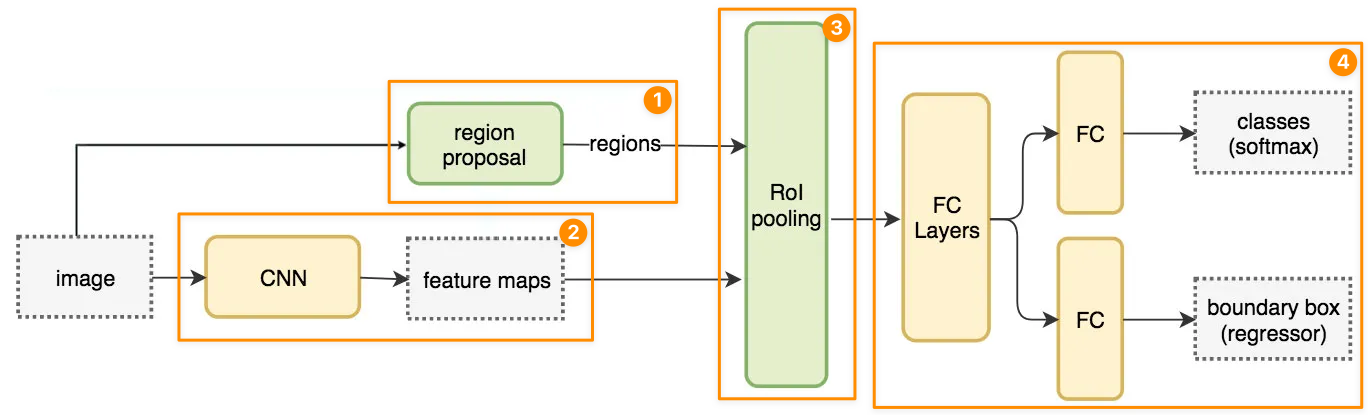
\includegraphics[width=5.5in]{figures/fast_rcnn_flowc.png} \label{fig:fast_rcnn_flowc} 
    }
    \caption{Fast R-CNN overall architecture and network flow} \label{fig:fast_rcnn_archite_flowc}
\end{figure}

The overall architecture of Fast R-CNN can be thought of as four stages [Fig. \ref{fig:fast_rcnn_archite_flowc}]. The network takes an image and a set of RoI as inputs. Comparing Fast R-CNN with R-CNN, which takes an image as an input and then generates RoIs with selective search, the type of input data between the two models is not equivalent. Thus we assume Fast R-CNN takes an image as input and performs the selective search algorithm as the first stage of the model. In the second stage, Fast R-CNN generates a feature map for the entire image by running the input image through a CNN. The CNN used for Fast R-CNN performance measurement in the original paper is VGG16. In the third stage, the model use RoIPool layer to extracts the feature grid corresponding to the proposed RoI from the image feature map generated in stage two for each proposed RoI. The RoIPool layer is also used for downsampling the RoI feature grid of any size to a pre-defined fixed-length feature vector. In the fourth stage, each RoI feature vector is processed by multiple fully connected layers and then branched into the two sibling output layers -- softmax classification and bounding box regression. The model's learning with two output branches is possible with the use of multi-task loss.

\begin{figure}[!ht]
    \centering
    \subfloat[][R-CNN architecture with stages]{ 
        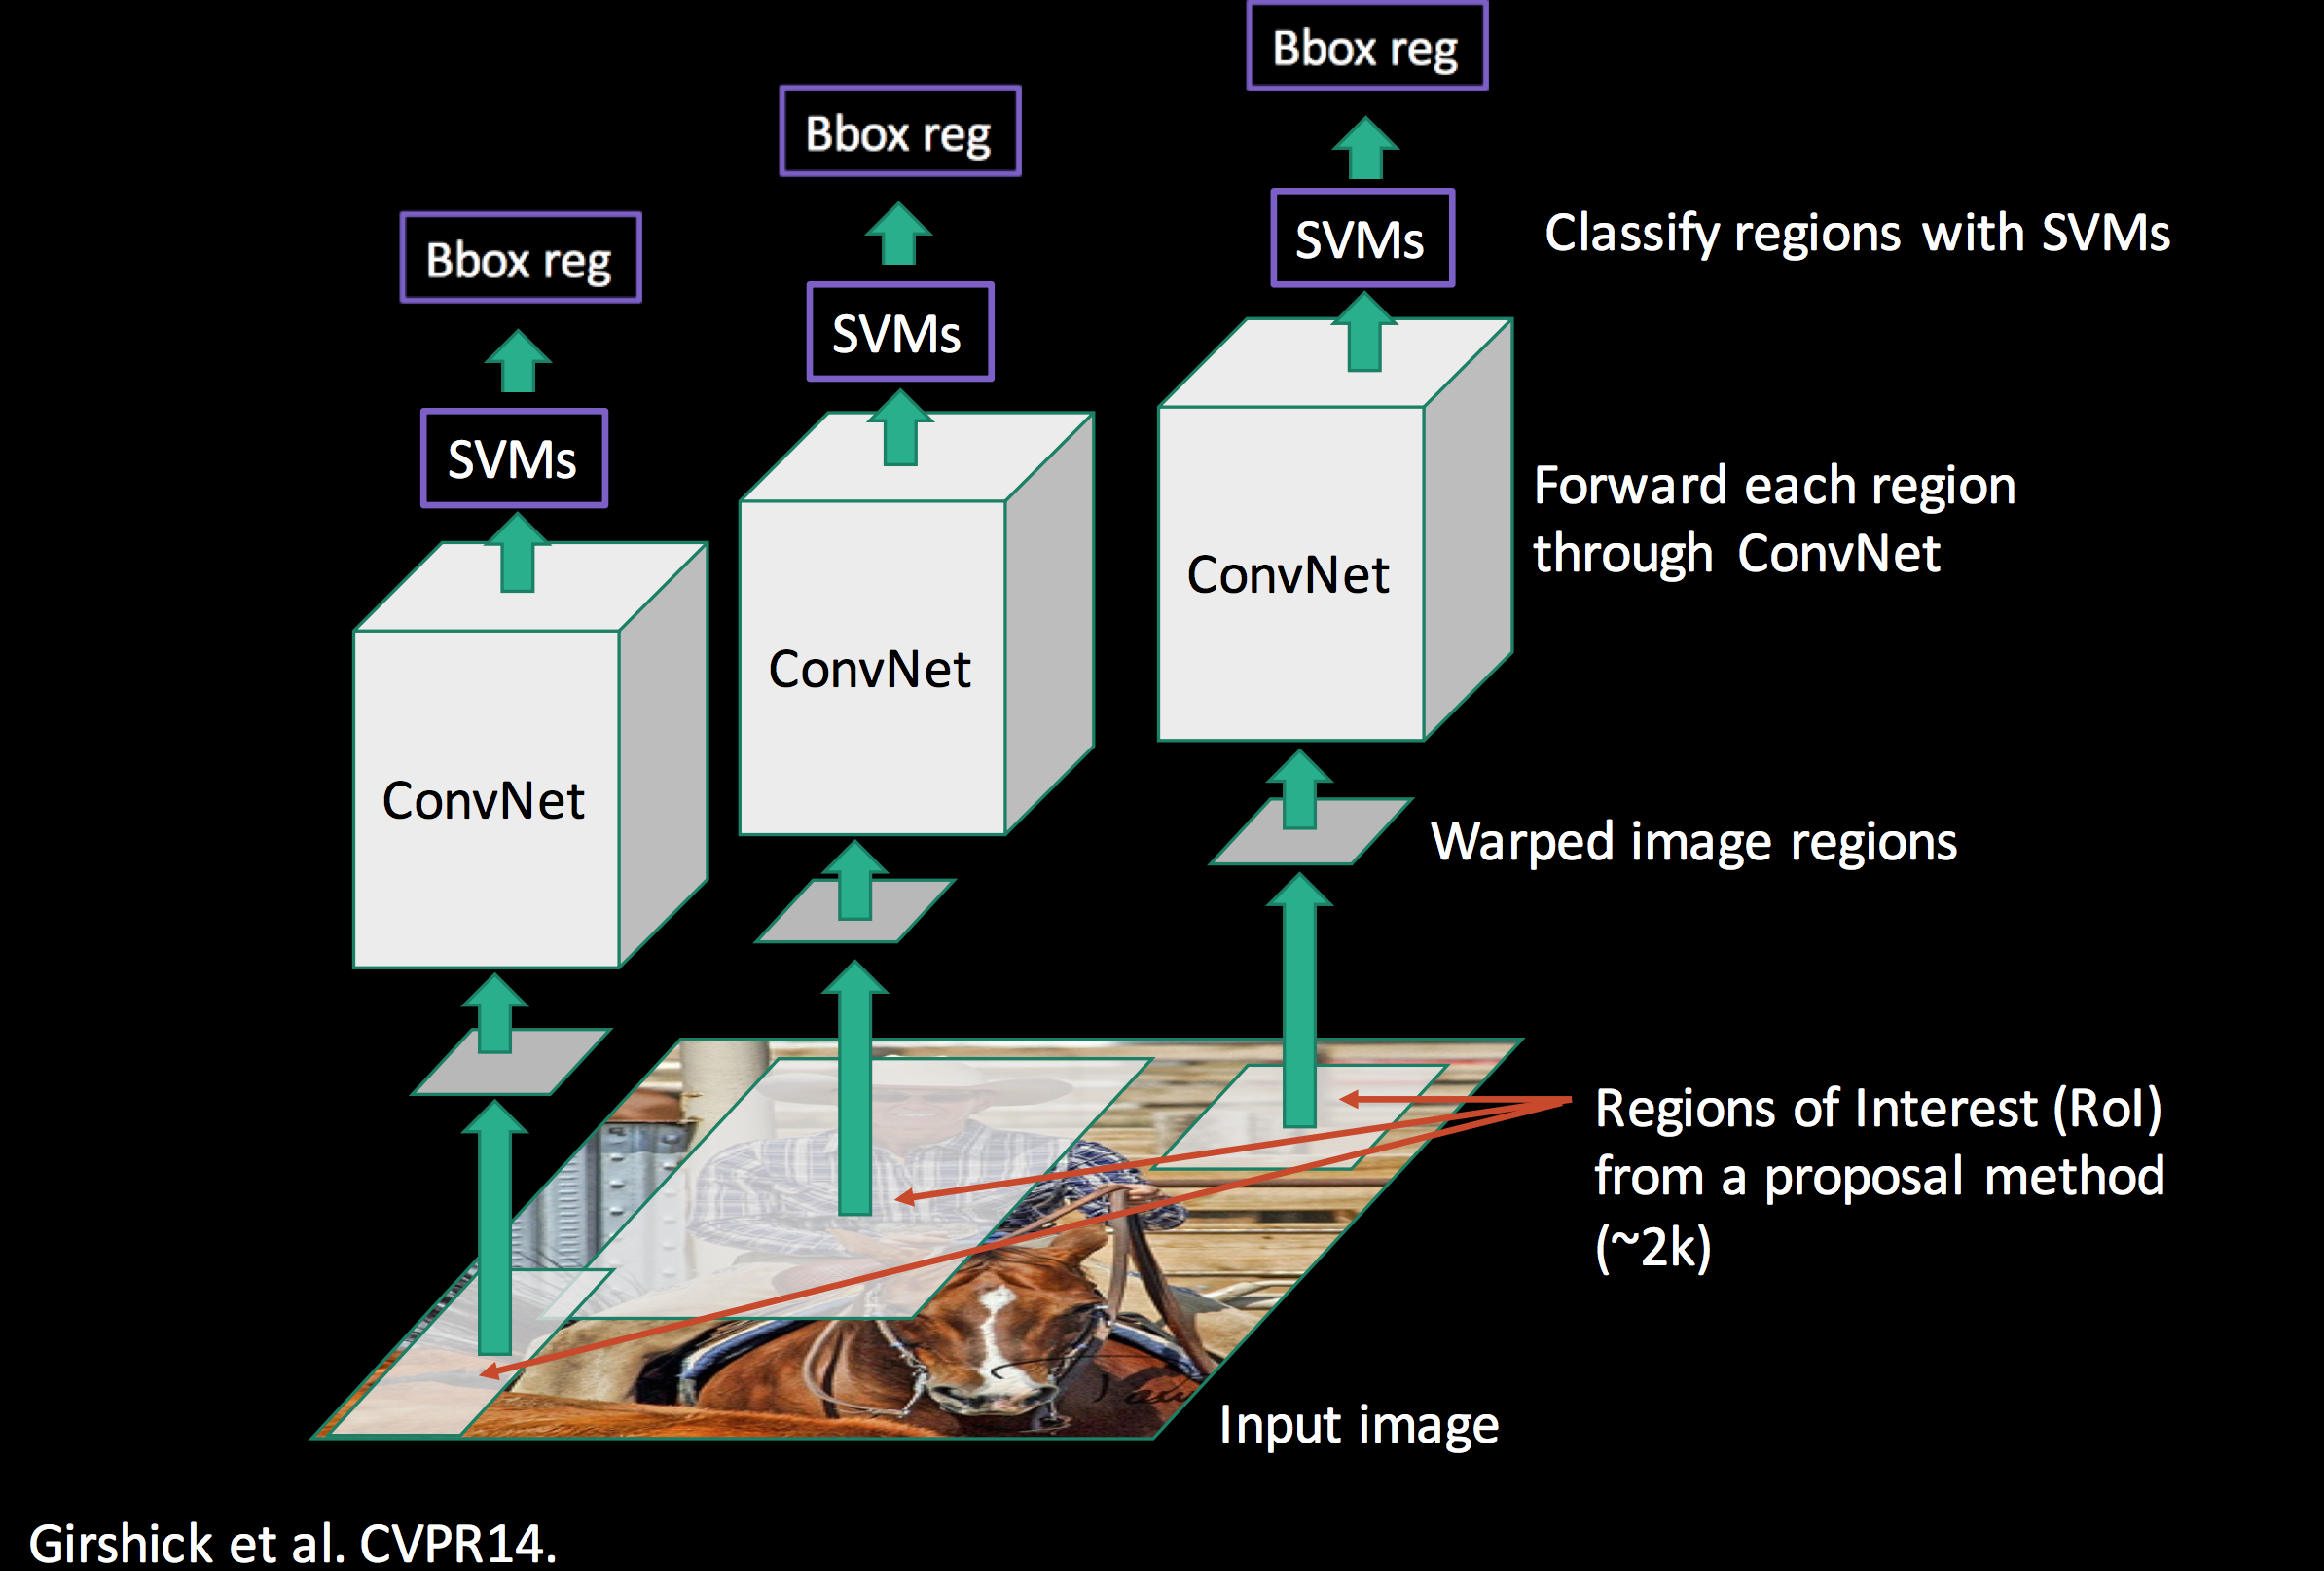
\includegraphics[height=2in]{figures/rcnn_custom_draw.png} \label{fig:rcnn_custom_draw} 
    }
    \subfloat[][Fast R-CNN architecture with stages]{ 
        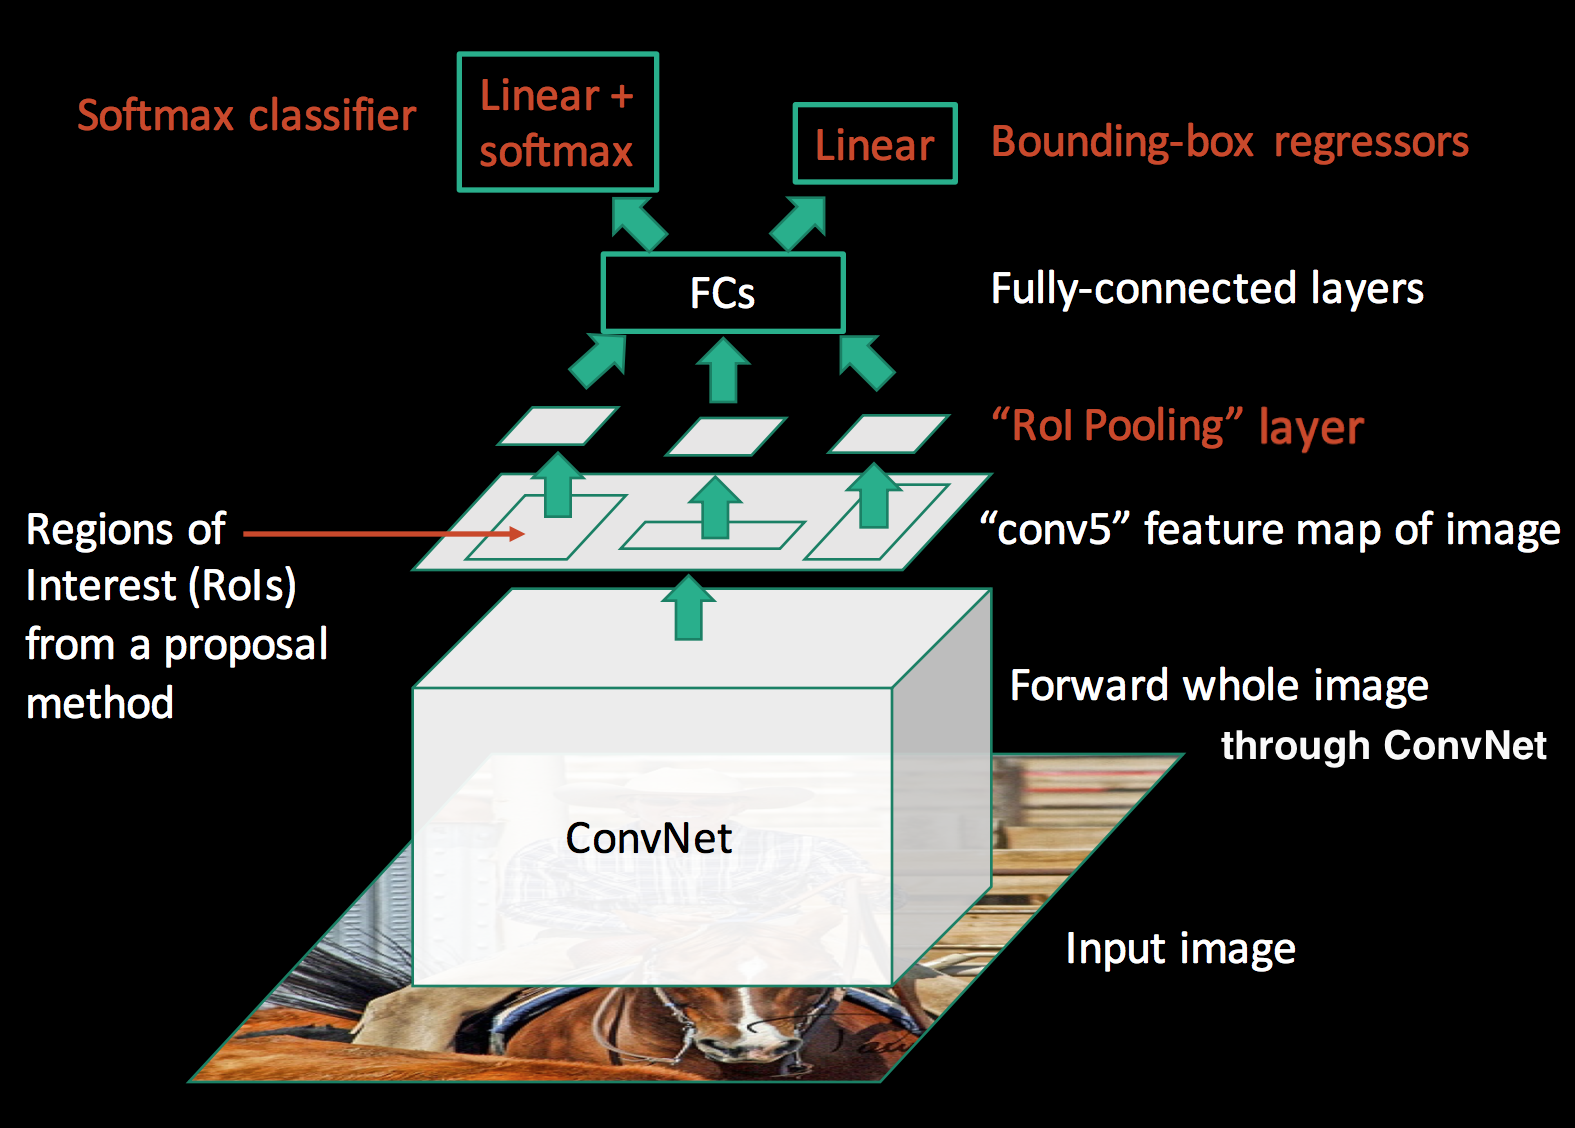
\includegraphics[height=2in]{figures/fast_rcnn_custom_draw.png} \label{fig:fast_rcnn_custom_draw} 
    }
    \caption{R-CNN vs. Fast R-CNN architecture comparision \cite{rcnn_vs_faster_custom_fig}} \label{fig:rcnn_vs_fast}
\end{figure}

Comparing the architecture of R-CNN and Fast R-CNN, there are three main differences between the two models [Fig. \ref{fig:rcnn_vs_fast}]. The first difference is that Fast R-CNN generates the feature map for the entire input image instead of each RoI individually. This means Fast R-CNN only applies CNN to image one and shares the feature maps across RoIs. Fast R-CNN behavior holds several advantages compared to treating RoIs individually, like in the R-CNN model. These advantages are reducing the use of disk storage, reducing redundancy operation performed on overlapping RoI, and sharing computation power and memory used between RoIs in the same image, thus improving the performance at test-time \cite{fast_rcnn_og}. Sharing the feature map and memory data between RoIs also allows the model to be trained faster. The author reported that training Fast R-CNN by examining multiple RoIs in an image allows the model to convert roughly 64 times faster compared to when trained with RoIs from different images. 

The second difference is the inclusion of the RoI pooling layer (named RoIPool). This layer is responsible for extracting RoI feature grids of varying sizes and downsampling them to a fixed pre-defined size. To extract the RoI feature grid for any input RoI, the RoIPool layer first maps the top left corner point of the input RoI box, which is defined on the input image, to a corresponding pixel in the feature map. Then, the width and height of the input RoI are reduced by the same factor that the feature map is downsampled from the original image. As we will perform a max-pooling operation on the pixels' value, the size of the original projected RoI must be rounded down to the nearest integer because we cannot take a partitioned pixel. After projecting the top left corner and rounding the scaled-down RoI size from the input layer onto the feature map, we have the offset rounded projected RoI. The RoI feature grid is then formed by every feature map pixel that lies inside this offset rounded projected RoI. Since objects in the input image can have different sizes and aspect ratios, thus the projected RoI feature grid can also vary in size. However, the input of a fully connected layer must be of the same pre-defined size, which is why the input's size independent downsampling operation is necessary. The RoIPool layer achieves size-independent downsampling by dividing the RoI feature grid into a pre-defined $W \times H$ grid of RoI bin (or RoI bin), where $W \times H$ is the required dimension for the following fully connected layer input. In other words, the layer divides the $w \times h$ RoI feature grid into RoI bins of equal size, each with an approximate size of $\frac{w}{W} \times \frac{h}{H}$. Here, $\frac{w}{W}$ and $\frac{h}{H}$ represent the number of pixels along the width and height of the RoI bin, respectively, and are rounded down to the nearest integer. In contrast to the traditional pooling layer described in Sec. \ref{subsec:pooling_layer}, which used a sliding technique dependent on the input size, the division into a grid of equal RoI bins enables the RoIPool layer to have a fixed output grid size regardless of the size of the layer's input RoI. The RoIPool layer then applies max-pooling to the pixel values in each RoI bin, thereby effectively reducing the size of any projected RoI to a pre-defined $W \times H$ size.

The third difference is going from multi-stage training in R-CNN to single-stage multi-task training in Fast R-CNN. In R-CNN, the model must be completely trained with class-specific SVM before being trained with class-specific bounding box regressor, and these tasks also are performed in the same sequence in the test time. On the contrary, Faster R-CNN has the softmax classifier and bounding box regressor as sibling output layers. Fast R-CNN model generates a multi-task loss $L$ for each RoI and uses the loss $L$ as a metric to jointly train both the softmax classifier and bounding box regressor branches. The multi-task loss $L$ is generated from the difference between the truth label, truth box, and predicted label, predicted box perspectively. The author suggested that employing a multi-task learning scheme would improve performance, as the network's shared components must be general and precise enough to produce correct results for both classifier and bounding box regressor branches \cite{fast_rcnn_og}. The author also reports that Fast R-CNN with multi-task learning consistently achieved higher mAP scores than stage-wise training across different CNN implementations.

These changes in architecture allow the Fast R-CNN model to achieve a processing runtime of 0.3 seconds per image, excluding the time needed for object proposal \cite{fast_rcnn_og}. However, when factoring in the runtime for object proposal, such as the Selective Search algorithm, Fast R-CNN is almost 7.67 times slower, taking 2.3 seconds per image \cite{selective_search_2013}. Additionally, the RoIPool layer in Fast R-CNN causes the model to undergo quantization. Quantization is the process of reducing the precision of an input from a large set of possible values to a smaller set of discrete values. Recall that the RoIPool layer initially projects the input RoI box to the appropriate location, rounded down to the nearest pixel in the feature map. The layer then subdivides the projected RoI, expressing the size of each RoI bin in the projected RoI in terms of pixels. In other words, the RoIPool layer quantizes these sizes and coordinates from the continuous non-negative real number set to the discrete natural number set. While quantization enables the layer to perform a valid max-pooling operation on pixel values, it also introduces a loss of precision and information in our model. The loss in precision is caused by the projected RoI deviating slightly from its actual coordinate. The loss in pixel data is due to the RoI RoI feature grid cannot always be divided perfectly without remainder.

\begin{figure}[!ht]
    \centering
    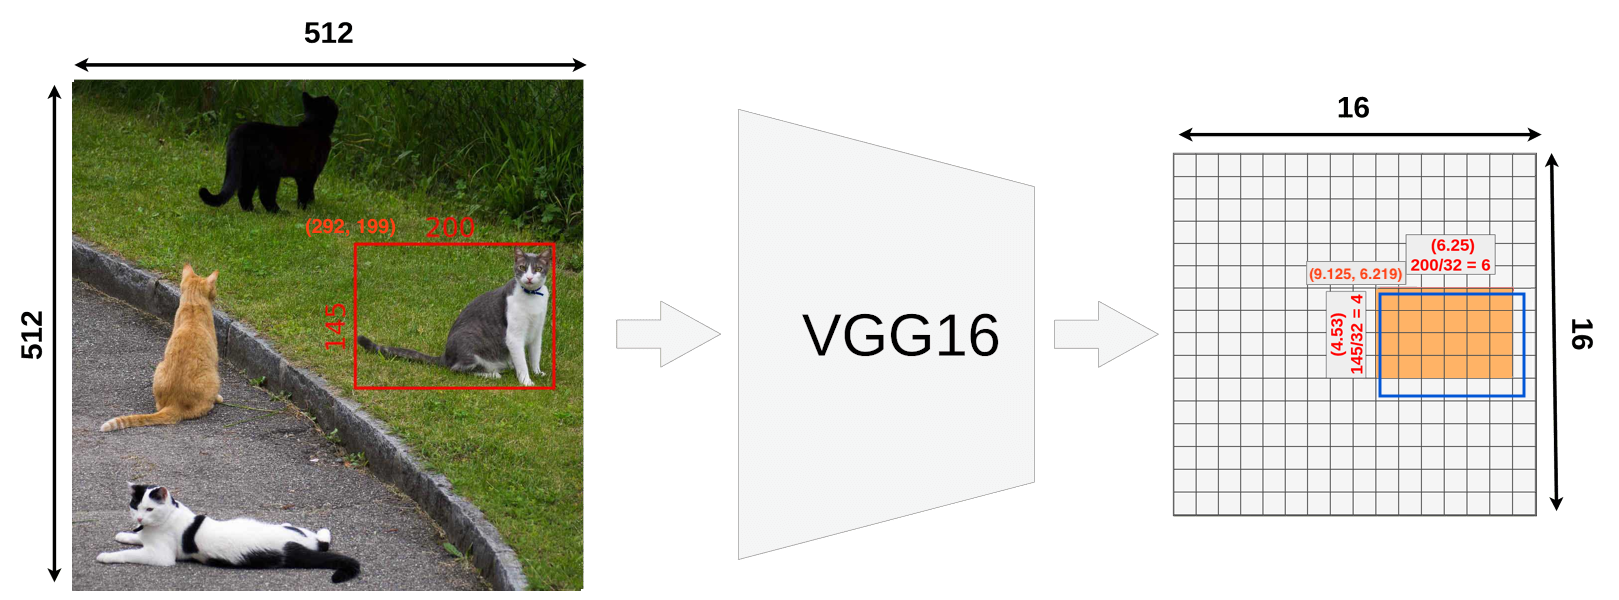
\includegraphics[width=6in]{figures/roi_projection_ex.png}
    \caption{RoI projection to feature map \cite{roi_pooling_problem}}
    \label{fig:roi_projection_ex}
\end{figure}

As an example, assume that we are processing an input image of $512 \times 512$ with VGG16, and the first fully connected layer expects $3 \times 3$ as input [Fig. \ref{fig:roi_projection_ex}]. Consider the input RoI with the top left corner coordinate of $(292, 199)$ and the size of $145 \times 200$. As mentioned earlier, VGG16 has a scale-down factor of $32$ from the input image to the feature map space. With this information, we can compute the corresponding coordinate and size of the input RoI in the feature map as follows:
\begin{align}
    &\text{Feature map RoI corner coordinate: } &\left( \floor{\frac{292}{32}}, \floor{\frac{199}{32}} \right) \ \ &= \ \ \left( \floor{9.125}, \floor{6.21875} \right) \ \ &= \ \ (9, 6) \\
    &\text{Feature map RoI size: } &\floor{\frac{200}{32}} \times \floor{\frac{145}{32}} \ \ &= \ \ \floor{6.25} \times \floor{4.53125} \ \ &= \ \ 6 \times 4
\end{align}
When projecting to the feature map space, Fast R-CNN offsets and resizes the original projected RoI (shown as the blue rectangle in Fig. \ref{fig:roi_projection_ex}) to align perfectly with $n$ feature map pixels (shown as the orange area in Fig. \ref{fig:roi_projection_ex}), where $n$ is the number of feature map pixels that can fit entirely within the original projected RoI. As shown in Fig. \ref{fig:roi_projection_ex}, we lose some pixels data (white part inside the blue rectange), and have additional noise datas (orage part outside the blue rectange). Consider the quantization of the conner's vertical position at 6.21875 to 6 in feature map space. When we factor in the scaling of 32 times, this means our projected RoI is shifted by $(6.21875 - 6) \times 32 = 7$ pixels vertically compared to the input RoI in the original image space. Similarly, the projected RoI is offset by 4 pixels horizontally, and the quantization process results in a loss of $(0.25 + 0.53125) \times 32 = 25$ pixels during projection.

\begin{figure}[!ht]
    \centering
    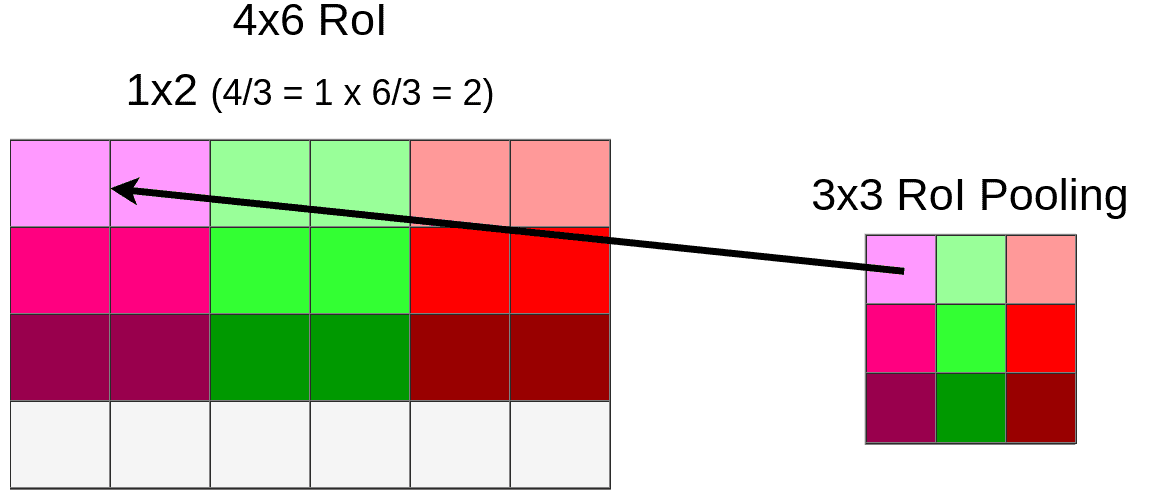
\includegraphics[width=4in]{figures/roi_pool_ex.png}
    \caption{The RoI feature grid is divided into RoI bins, as shown on the left. Performing max-pooling on each RoI bin results in a $3 \times 3$ output matrix, as shown on the right. Each cell in the input image represents a feature map pixel, and each RoI bin contains 2 pixels and has a unique color. Each cell in the output $3 \times 3$ matrix represents the highest feature map pixel out of all pixels in each corresponding RoI bin. The white cells on the left do not belong to any RoI bin and are not used in the RoI pooling process.\cite{roi_pooling_problem}}
    \label{fig:roi_pool_ex}
\end{figure}

After projecting and quantizing the input RoI, we obtain an RoI feature grid. In our example, this grid has dimensions of $6 \times 4$ and is located at position (9, 6). However, the next layer in our network requires inputs of size $3 \times 3$. To accommodate this, we divide the RoI feature grid into a grid of RoI bins, each with a size of $\frac{6}{3} \times \frac{4}{3} \approx 2 \times 1.3333$. Since these sizes are expressed in terms of pixel counts, we must quantize them to the nearest integer values, resulting in RoI bins of size $2 \times 1$. As shown in Fig. \ref{fig:roi_pool_ex}, this quantization results in the loss of information for the bottom row of pixels in the RoI feature grid, corresponding to a loss of $6 \times 32 = 192$ pixels in the input image space. In addition, the pooling operation can also cause small offsets in the position of the RoI bins, leading to further loss of information. Combined every loss happen in the RoIPool layer, the model has loss $192+25=217$ pixels. In addition, the RoI used for classification is offset by 7 pixels vertically and 4 pixels horizontally. While the loss of 217 pixels due to quantization and pooling may seem small compared to 29,000 pixels in the input RoI of size $200 \times 145$, thereby, can be overlooked in the object detection task. However, as the goal of our study lies in the instance segmentation task, where the model outputs a mask containing every pixel belonging to the object, every pixel counts. Nonetheless, these loss in information and offset is for one input RoI. Due to the fact that object identification tasks typically detect multiple objects per image, the loss of information and offset caused by quantization may compromise the quality of the model. 

To address the quantization issue in the RoIPool layer, RoIAlign was proposed as a method for achieving size-independent downsampling without quantization. The RoIAlign is utilized with Mask R-CNN, an instance segmentation model that will be discussed in greater detail in Sec. \ref{sec:mask_rcnn}. Since Mask R-CNN is built on top of Faster R-CNN, which is also the subsequent significant improvement over the Fast R-CNN model, we will discuss the Faster R-CNN model in the following section. Faster R-CNN proposes the addition of the region proposal network (RPN) to resolve the bottleneck in object detection performance caused by object proposal runtime \cite{faster_rcnn_2015}. Instead of attempting to reduce the runtime of the object proposal algorithm, RPN's primary objective is to share computation with the object classification module, thereby allowing the object detection model to generate object proposals at no additional cost. We will further discuss the region proposal network (RPN) used in conjunction with Fast R-CNN to create Faster R-CNN in section \ref{sec:faster_rcnn}.

\section{Faster R-CNN}

\section{Mask R-CNN} \label{sec:mask_rcnn}
%!TEX root = ../username.tex
\chapter{YOLO Variation} \label{chap:yolo_variation}

In addition to the Region-based Convolutional Neural Network (R-CNN) family, the other family of model we will discuss in this section is You Only Look Once (YOLO). Similar to R-CNN family, YOLO family also designed to perform object detection and can be expand to other task like instance segmentation or semantic segmentation. However, unlike R-CNN family, the model in YOLO family frame the object detection task as a single stage regression problem instead of double stage regression problem {\color{red} cite yolov3}. 

The models in R-CNN family is consider as double stage method because the model first try to generate region of interest (RoI), then classify each ROI using two different algorithm or network. That is, while RoI generation can be done with a greedy algorithm (like Selective Search) or a fully connected convolutional network (like RPN), the model use another CNN for feature extraction (like AlexNet, VGG16, and ResNet) and adapt it to perform classfication for each generated RoI \cite{Girshick_R_CNN_2013, fast_rcnn_og, faster_rcnn_2015}. For this reason, the object detection task is seperate into two tasks: localization task and classfication task, where each task is completed by a different network.

On the other hand, the models in YOLO family is utilized a single convolution neural network to simultaneously predict both bounding box and the classfication label for each object in the input image \cite{yolov1_2016}. Therefore YOLO model family is designed to only evaluate an image once with a single CNN for object detection task. Hence the name You Only Look Once. In this chapter we will disscuss different version of YOLO model.

\section{YOLOv1}  \label{sec:yolov1}

The first YOLO model was proposed in the "You Only Look Once: Unified, Real-Time Object Detection" paper in 2015 \cite{yolov1_2016}. Since there will be improvement version of the model, we denote this first model is YOLOv1, which is widely accepted in the computer vision research community \cite{understand_cnn_vs_yolo}. The YOLOv1 is designed to be a realtime object detection model. The YOLOv1 model is a three steps process, as shown in Firgure \ref{fig:yolov1_process}. In the first step, the model take an image of any size as input and resize the image to the fix size of $448 \times 448$. In the second step, the model predict mutiple bounding box, each with a objectiveness confidence score, and multiple classification for each detected object. Since the model predict multiple bounding box and classfication for each detected object, a non-maximum suppression (NMS) algorithm, as described in Subsection \ref{subsec:rpn}, is applied to assign one bounding box and one classification label per predicted object in the last step.

\begin{figure}[!ht]
    \centering
    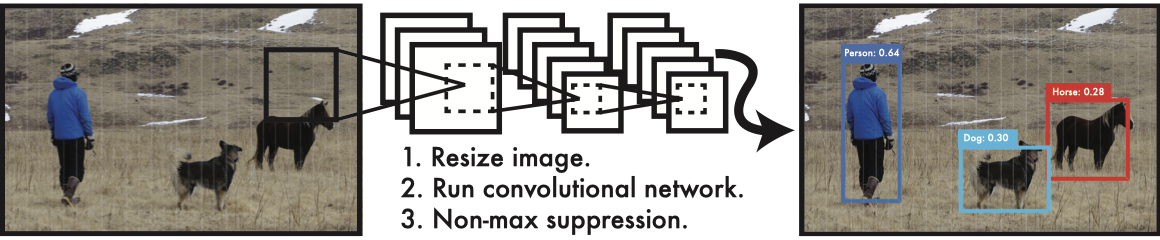
\includegraphics[width=4in]{figures/yolov1_process.png}
    \caption{YOLOv1 object detection process \cite{yolov1_2016}} 
    \label{fig:yolov1_process}
\end{figure}

In the original paper, the authors claim that YOLOv1 model have three main benifit \cite{yolov1_2016}. First, YOLOv1 is extremely fast, processing 45 images per second compare to 7 images per second achieved by the Faster R-CNN model with VGG16 backbone. However, this is achieved at the cost of 9.8\% reduction in mean average precision (mAP) score, i.e., 63.4\% and 73.2\% for mAP score of YOLOv1 and Faster R-CNN, respectively. The second benifit is YOLOv1 learn a general representation of object, thus it tend to perform better compare to R-CNN based model when predicting for other domain like artwork. The third benifit it it see the entire image during bounding box regression and classification compare to R-CNN classifier and bounding box regressor only see the ROI. This change allow YOLOv1 to encodes contextual information about classes and thus reduce the number of false positive.

\subsection{Network Architecture}

\begin{figure}[!ht]
    \centering
    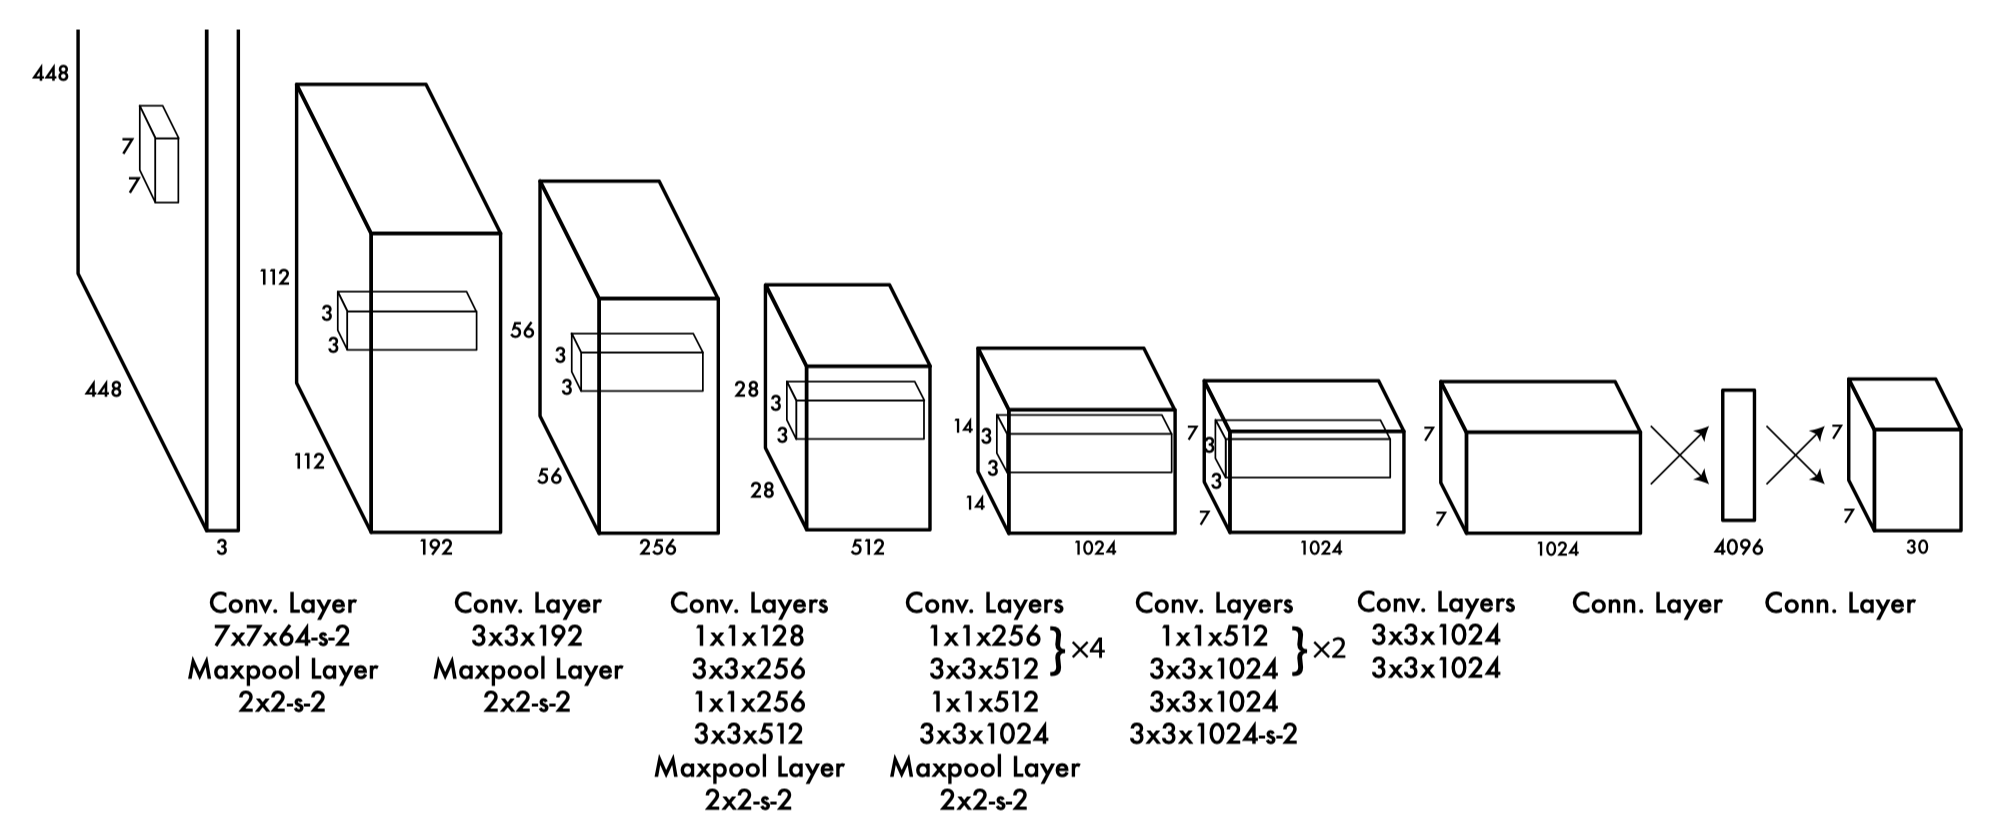
\includegraphics[width=4in]{figures/yolov1_archite.png}
    \caption{YOLOv1 architecture \cite{yolov1_2016}} 
    \label{fig:yolov1_archite}
\end{figure}

The YOLOv1 model is a convolutional neural network (CNN) based on the GoogLeNet model for image classification {\color{red} cite GoogLeNet}. The YOLOv1 model consist of 24 convolutional layer and end with 2 fully connected layer. The overall architecture of YOLOv1 netword is shown in Figure \ref{fig:yolov1_archite}. The author replace the inception layers in GoogLeNet with $1 \times 1$ reduction layer and $3 \times 3$ convolutional layer pair {\color{red} further explain the inception modules and reduction layer}. All the layers in the yolov1 network, with the exception of the final layer, utilize the leaky ReLU activation function {\color{red} cite leaky ReLU}, described as:
\begin{equation*}
    \phi(x) = {\color{red}x if x > 0, 0.1 x otherwise}
\end{equation*}

As we can see in Figure \ref{fig:yolov1_archite}, the last convolutional layers in the network produce a feature map of size $7 \times 7 \times 1024$. This feature map is then processed by two fully connected layers. The last fully connected layer is responsible for predicts both the bounding box and the class label probability \cite{yolov1_2016}. This layer use a linear activation function. The classfication process in the last fully connected layer is simmilar to other CNN where the layer is randomly initialize and can be optimized through training. On the other hand, YOLOv1 proposed a new bounding box regression method that able to  predict all bounding box of all objects present in the image at once, instead of processing each RoI individually one-by-one like the regressor implemented in Faster R-CNN. We will discuss this bouding box generation process in the next subsection.

\subsection{Bounding Box Generation}
To predict bounding box, the YOLOv1 model divide the image into an $S \times S$ grid of equal cells. Each grid cell is then predict $B$ bounding boxes and $C$ probabilities for the $C$ supported classes \cite{yolov1_2016}. The $S$ and $B$ values are hyperparameter and can be fine tune throught experiment. The $C$ value is the number of classes in the training dataset. In other words, $C=20$ if the training dataset is PASCAL VOC \cite{pascal_voc_2015} and $C=80$ if the training dataset is COCO dataset \cite{coco_2014}.

Each bounding box is represented by 5 values: coordinate $x$, coordinate $y$, width $w$, height $h$, and a confidence score. The $(x, y)$ coordinates is the center of the bounding box relative to a grid cell. The width $w$ and height $h$  is the dimension of bouding box in 2D space. The value of $w$ and $h$ are normalized with respect to the input image width and height, thus they are bounded by [0, 1]. The confidence score denote the model confidence in saying there is an object present in this cell, i.e., the objectiveness probability.

\begin{figure}[!ht]
    \centering
    \subfloat[][{\color{red} tobe added}]{ 
        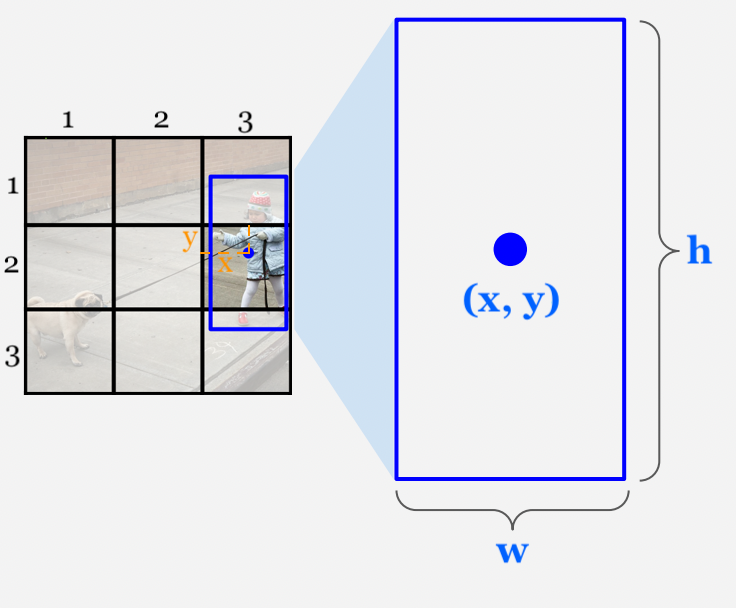
\includegraphics[height=2in]{figures/yolov1_bbox1.png} \label{fig:yolov1_bbox1}
    }
    \qquad \qquad
    \subfloat[][{\color{red} tobe added}]{ 
        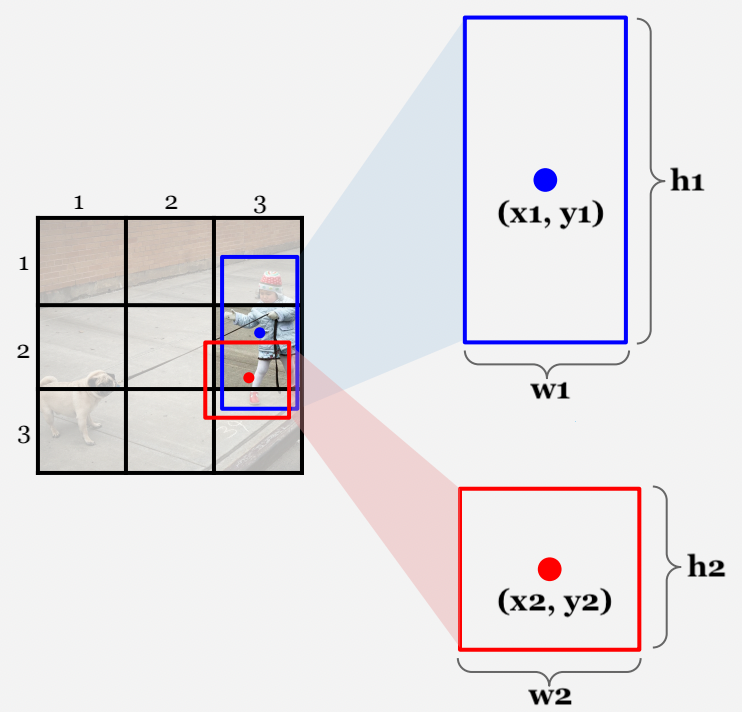
\includegraphics[height=2in]{figures/yolov1_bbox2.png} \label{fig:yolov1_bbox2}
    }
    \caption{{\color{red} tobe added}}
\end{figure}

As an example, consider processing an image with $S=3$, $B=1$, and clasifying between two class human and dog ($C=2$), as demonstrated in Firgure \ref{fig:yolov1_bbox1}. Since $B=1$, which means we only predict one bounding box per cell, then the cell$_{32}$ will return a tensor represent the predicted bounding box as:
\begin{equation*}
    ceil's\ output = \begin{bmatrix}
        {\color{blue} x \quad y \quad w \quad h \quad conf} \quad p_{human} \quad p_{dog}
        \end{bmatrix}
\end{equation*}
where $conf$ is the confidence score, $p_{human}$ and $p_{dog}$ are probability that the object belong to the human and dog class, respectively. Noted that when we only predicting 1 bounding box per ceil, the YOLOv1 model predict $(4+1+2)$ values for each ceil, where 4 value describe the bounding box location, 1 for confidence score, and 2 probality values with one for each class. Therefore we say that when $B=1$, the model predict $(4+1+C)$ for each ceil. 

Now, we consider the example reside in Figure \ref{fig:yolov1_bbox2}, which is the same setup as previous example but with $B=2$. In this second example, we predict two bounding boxes per cell, then the cell$_{32}$ return the following tensor for the two bounding boxes:
\begin{equation*}
    ceil's\ output = \begin{bmatrix}
        {\color{blue} x_1 \quad y_1 \quad w_1 \quad h_1 \quad conf_1} \quad 
        {\color{red} x_2 \quad y_2 \quad w_2 \quad h_2 \quad conf_2} \quad 
        p_{human} \quad p_{dog} 
    \end{bmatrix}
\end{equation*}
The ceil output a $(4+1)*2+C$ elements tensor for when the model predict two bounding boxes per ceil. Therefore, we can generalize the ceil's prediction is encoded as $(4+1)*B+C$ tensor.

The computed prediction for each ceil in the grid is stacked side by side create the depth for the image. That is we divides a 2-dimentional image into a grid of $S \times S$ ceil, we predict a $(4+1)*B+C$ tensor for each ceil, these prediction create the third dimention of the image. Therefore the prediction for the image is encoded as $S \times S \times [(4+1)*B+C]$ tensor. 

The YOLOv1 architecture showned in Figure \ref{fig:yolov1_archite} is for predicting 20 class in PASCAL VOC with $S=7$ and $B=2$, thus the model predicting a $7 \times 7 \times 30$ tensor which encoded multiple bouding boxes and classfication for each ground-truth object. 

\subsection{Training}
The first 20 convolutional layers of YOLOv1 is pretrained with the input size of $224 \times 224$ for classification task on the ImageNet2012 dataset \cite{ImageNet_dataset}. Then four new convolutional layers and 2 fully connected layer are added. These new layers are randomly initialize. Additionally, the input size is increase to $448 \times 448$ for object detection task \cite{yolov1_2016}. With the initialized network, the model generate multiple bounding boxes and classification as described previously. While the YOLOv1 model apply NMS to choose which predicted bounding box to keep at inference time, the author used a different scheme to choose which predicted bounding box to contribute to the loss function. The scheme is choosing the predictor with predicted box that has the highest IoU with a ground truth box. This lead to each predictor have different specilization, which mean each predictor is better at predicting certain size, aspect ratio, or object's class \cite{yolov1_2016}.

The YOLOv1 model is trained to optimize for the sum-square error which encode both the bounding box coordinate loss and the classification loss \cite{yolov1_2016}. While sum-square error allow eazier optimization, it have some shortcomming and not ideal if the model need to optimize for average precision. The first critical shortcomming is the loss weight localization error and classification error equally \cite{yolov1_2016}. In an image, since the majority of the cells does not contain any object, which mean confidence score for these cell are 0, thus cause model always have a poor performance for classification task. This also cause bouding box error to have little affet on the total error. Thus a scalar term is added to the loss to weight the bouding box error higher than the classification error \cite{yolov1_2016}. The second critical shortcomming is sum-squared error weight offset in large bounding box and small bounding box equally \cite{yolov1_2016}. This is not ideal as offset by certain pixels have a larger affect on the smaller bouding box than the larger bounding box, due to total number of pixels in large bounding box is larger than the smaller bounding box. To patially resolve this, the YOLOv1 model perform the error calculation on the squareroot of bounding box width and height instead of the width and height directly.

\section{YOLO9000 (YOLOv2)}  \label{sec:yolov2}

YOLO9000, also known as YOLOv2, is an improvement of the YOLOv1 model \cite{yolo9000_2017}. The real-time object detection model YOLOv2 was first introduced in 2016. The name YOLO9000 stems from the fact that the model is capable of detecting over 9,000 object categories in real time,  which is significantly more than the original YOLO model. This is achieved by finetuning the model with the WordNet language database, which also is the database that the ImageNet labels set pulls from.

\subsection{Accuracy Improvement}
The YOLOv2 model proposes five changes that improve the accuracy of YOLOv1. The first change is the addition of \textbf{batch normalization} on the convolutional layer, which improves the YOLOv1 mAP score by more than 2\%. Batch normalization removes the need for dropout technique \cite{dropout_2014}, which drops certain activated neurons to avoid overfitting problem \cite{szeliski_cv_book}. The second change is utilizing \textbf{higher resolution classifier}. While YOLOv1 only trains on $224 \times 224$ images for the classification task, YOLOv2 further trains the classifier with $448 \times 448$ images. The higher resolution classifier increases the YOLOv1 mAP score by 4\%. The third change is the use of \textbf{passthrough layer}. Since the convolutional layer decreases the image's spatial dimension gradually, thus it becomes more difficult to detect smaller objects in the image as more convolutional layers are used. For this reason, the passthrough layer help brings the image detail from the higher spatial dimension to the lower spatial dimension map, similar to the skip connection in ResNet \cite{resnet_2016}.

Since each divided cell in YOLOv1 only predicts exactly 2 bounding boxes, 1 confidence score, and 1 classification label (the highest probability class), thus the model has poor performance in detecting objects that appear near together, especially small objects. To address this problem, the YOLOv2 model proposes the fourth and fifth changes. 

The fourth change is utilizing \textbf{anchor boxes} at each cell instead of randomly initializing the bounding box like in YOLOv1. The size and aspect ratio of the anchor box heavily depends on the domain that the model will be applied to. For example, when applying the model to the traffic detection task, then the main shape and size the model need to look for are pedestrian and different vehicle. Thus starting the anchor box at these shape and size improve the runtime for both training and inference. For this reason, a k-means clustering algorithm is used to find the top-k common dimension in the training set \cite{yolo9000_2017}. The anchor boxes are then used to predict the bounding box. The YOLOv2 model predicts five parameters for each bounding box $[t_x, t_y, t_w, t_h, and t_o]$, where $t_x, t_y$ and $t_w, t_h$ is the center and the dimension of the bounding box in relation to the cell and the image dimension, respectively. These five parameters are the same as the prediction made by YOLOv1. Given that the cell is $(c_x, x_y)$ offset from the top-left corner of the image, and the anchor box has the dimension of $p_w, p_h$, then the predicted bounding box has the center at $(b_x, b_y)$ with the dimension of $b_w, b_h$, and can be computed with constraint by sigmoid function, as shown in Figure \ref{fig:yolov2_bbox}.

\begin{figure}[!ht]
    \centering
    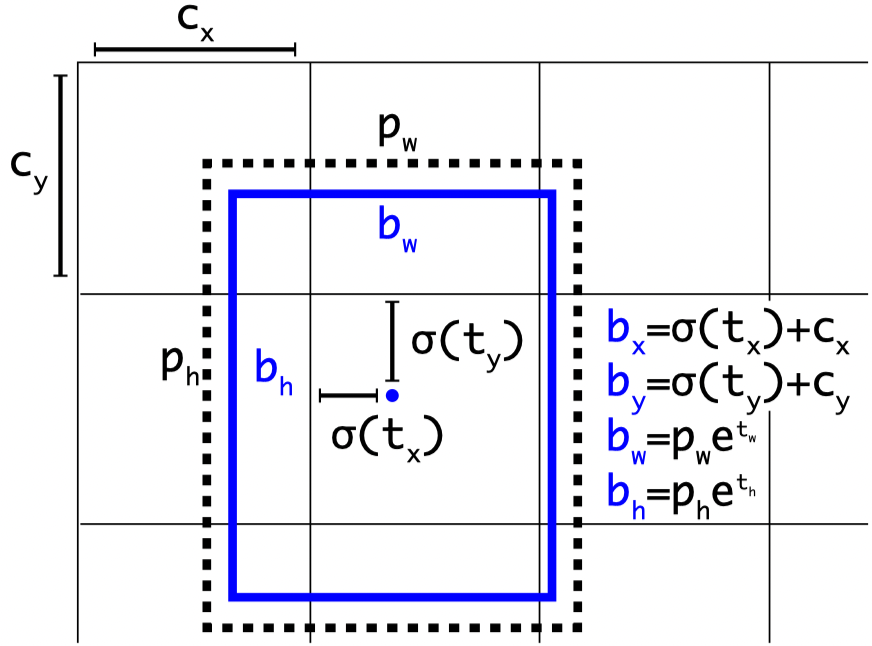
\includegraphics[width=3in]{figures/yolov2_bbox.png}
    \caption{YOLOv2 bounding box (in blue) generation offset from the anchor box (in black) \cite{yolo9000_2017}} 
    \label{fig:yolov2_bbox}
\end{figure}

Since the anchor boxes are used to predict the bounding box, this removes the need for fully connected layers. In addition to the removal of fully connected layers, the YOLOv2 model also moves the classification label from the cell level to the anchor box level. In other words, the YOLOv2 model predicts a classification label for each anchor box \cite{yolo9000_2017}. Let the image be divided into an $S \times S$ cell grid, each cell generates $B$ anchor boxes, and the dataset has $C$ categories, then the image detection is encoded as a $S \times S \times B*(4+1+C)$ tensor. The anchor box scheme removes the assumption of one object per grid cell and improves the mAP score by approximately 5\%.

The fifth change is \textbf{multi-scale training}. Since YOLOv2 remove the fully connected layer, thus it can process images of any size. Therefore, instead of training with a fixed size, the model chooses a new input image dimension every 10 batches. Additionally, since the model is downsampled by 32 times during its process, to avoid quantization, the input image should be a multiple of 32: {320, 352, ..., 608}. This training scheme forces the model to be able to predict object at different resolutions, which train the network to predict object of different scale. In addition to multi-scale training, the model also performs a data augmentation process, including crop, rotation, hue and saturation shift, and exposure shifts to expand the training dataset and further generalize the model.

\subsection{Runtime Improvement}
The YOLOv2 further simplifies the architecture used in YOLOv1. The YOLOv2 model uses a new classification model, namely Darknet-19. The overall architecture of Darknet-19 is shown in Figure \ref{fig:darknet19_archite}. Compared to the GoogLeNet, Darknet-19 is smaller, with 5.58 billion operations instead of 8.52 billion operations, while having higher top-5 accuracy in classification tasks after training \cite{yolo9000_2017}. Compared to YOLOv1's CNN architecture, Darknet-19 only has 19 convolutional layers and 5 max-pooling layers, while YOLOv1's CNN consists of 24 convolutional layers, 4 max-pooling layers, and 2 fully connected layers. The Darknet-19 is first trained with the ImageNet 1000 for the classification task. The Darknet-19 model is then adapted for the object detection task by replacing the last convolutional layer with three $3 \times 3$ convolutional layers that output 1024 channels, followed by $1 \times 1$ convolutional layer to convert $S \times S \times 1024$ to $S \times S \times B*(4+1+C)$.

\begin{figure}[!ht]
    \centering
    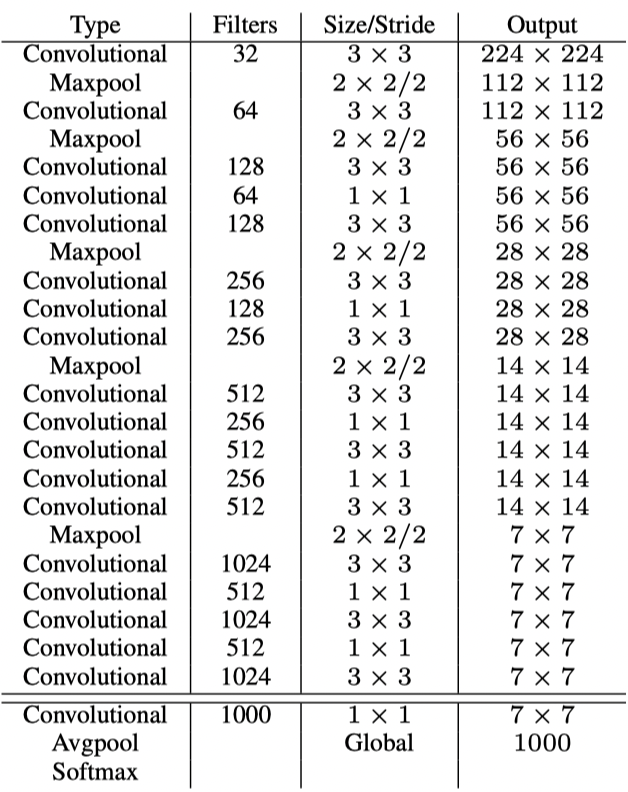
\includegraphics[width=4in]{figures/darknet19_archite.png}
    \caption{Darknet-19 architecture \cite{yolo9000_2017}} 
    \label{fig:darknet19_archite}
\end{figure}

\section{YOLOv3}  \label{sec:yolov3}

The YOLOv3 model is the next incresemental improvement of YOLO family after YOLO9000. The YOLOv3 model is introduced in 2018 \cite{yolov3_2018}, which consist of four main minor changes to YOLOv2 archietecture. 

The first change is replacing the softmax function with independent logistic for the classifier. While the softmax function require the sum of all class's probabilities to 1, independent logistic consider each class independently and the probability of any two class do not affect one another \cite{yolov3_2018}. This improve the model's classifier from multi-class classifier to multi-class and multi-label classifier. That is, when the classifier is multi-class and multi-label, there are no competition between label. For example, if a pedestrian is a women and the supported label include both "pedestrian" and "women", then when use  independent logistic classifier the probability for both label should be high for this object, while softmax classifier will only give high probability to one of the two labels.

While the format of the predicted bounding in YOLOv3 is the same as YOLOv2 (Figure \ref{fig:yolov2_bbox}), the calculation of the confidence score and loss function are different compare to YOLOv2. This is the second change the YOLOv3 proposed compare to YOLOv2. The YOLOv3 predicts the bounding box's confidence (objectness) score is predicted using a logistic regression \cite{yolov3_2018}. This is trained by setting the confidence score of the bounding box anchor to 1 if the anchor box has highest IoU score with the ground-truth box compare to other anchor. During training any anchor box that has IoU score more than 0.5 with a ground-truth box but the IoU score is not the highest among anchor boxes for this object, then that anchor box will not contribute to the loss function. If the model does not predict a bounding box anchor for a ground-truth object, the objectness loss will increase and contribute no affect to localization loss and classification loss. Simmilar to YOLOv1 and YOLOv2, YOLOv3 also optimize for sum-square error loss which combine the localization, classification, and objectness loss into one metric. 

The third change is detection at 3 different scales per cell. At each cell, the model predict $B$ bounding box for each feature map scale i.e., the current feature map and two upscaled feature map. Assume we divide the image into $S \times S$ cells and the dataset is COCO 80 labels, then at each scale the model predict $S \times S \times [3_{bbox} * (4 + 1 + 80)]$, thus the model generate a $S \times N \times [3_{scale} * 3_{bbox} * (4 + 1 + 80)]$ \cite{yolov3_2018}. The YOLOv3 model predict 9 anchor boxes per cell. This 9 anchor boxes is choosen using the k-means clustering algorithm and divided into each scale evenly. For example, the YOLOv3 model trained for COCO dataset will have the following 9 anchor boxes:
\begin{align*}
    Scale-1: &[(10 \times 13), (16 \times 30), (33 \times 23)] \\
    Scale-2: &[(30 \times 61), (62 \times 45), (59 \times 119)] \\
    Scale-3: &[(116  \times  90), (156  \times  198), (373  \times  326)]    
\end{align*}
    
The fourth change is the feature extractor. Inspired by Darknet-19 and ResNet, the author proposed a new CNN archietecture, namely Darknet-53. The overall architechture of Darknet-53 is shown in Firgure \ref{fig:darknet53_archite}.The network consist of 53 convolutional layers, $3 \times 3$ or $1 \times 1$ convolutional layers, and using shortcut connections \cite{yolov3_2018}. The shortcut connections is introduced in ResNet model and is used to skip over certain convolutional layers based on certain conditions, which improve runtime and address problems with high-depth networks \cite{resnet_2016}. The Darknet-53 is two times faster than the ResNet-152 model while perserve the model's accuracy. Other than the loss computation method, the Darknet-53 training is the same as YOLOv2 which include batch normalization, multi-scale training, and data augmentation.
\begin{figure}[!ht]
    \centering
    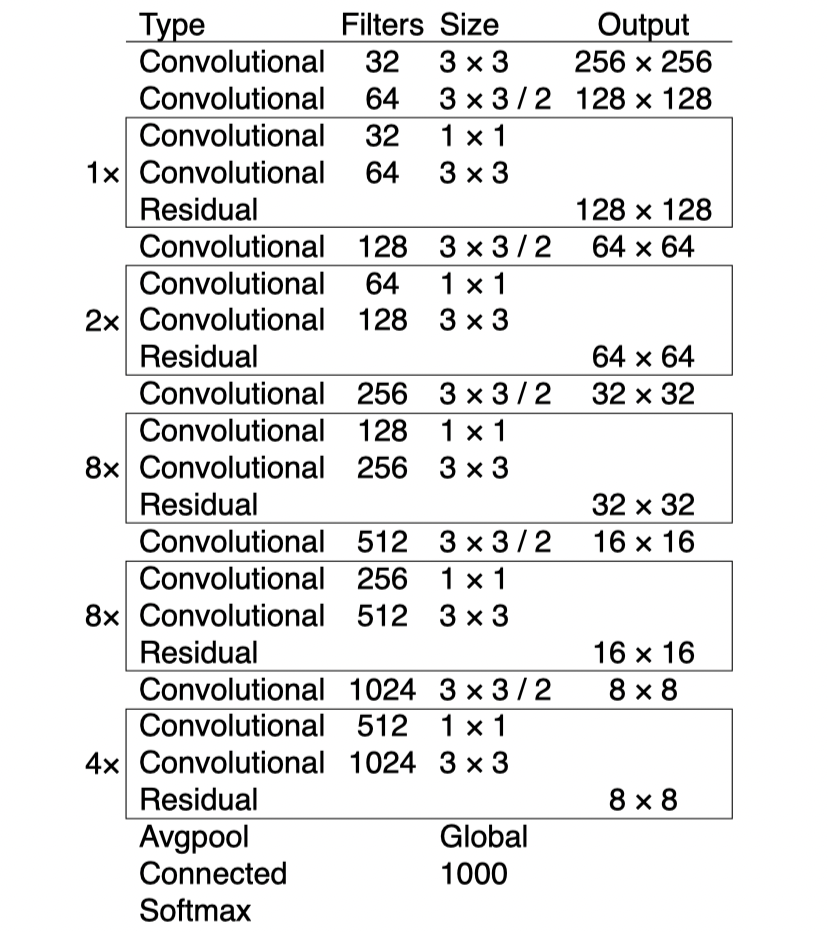
\includegraphics[width=3in]{figures/darknet53_archite.png}
    \caption{Darknet-53 architecture \cite{yolov3_2018}} 
    \label{fig:darknet53_archite}
\end{figure}

\section{YOLOv5}  \label{sec:yolov5}

The YOLOv5 is the fifth entry of the YOLO family. The model is published in 2020 by Ultralytics teams \cite{yolov5_github}. The name YOLOv5 is still controlversal to this date because it is considered as less innovative compare to the YOLOv4 model. While YOLOv4 has a significant change in structure and use some state-of-art algorithm like MISH activation function and GIOU(Generalized Intersection over Union) loss function, YOLOv5 is more focus on ease of use, model size control, and enhancing training data \cite{yolov5_review}. Unfortunately, YOLOv5 model have never had a formal research paper detail explaining the implementation detail, but it has a well documented and supported API developed and maintain by the Ultralytics teams \cite{yolov5_github}. 

At it core, YOLOv5 is YOLOv3 structure with flexible control of model size \cite{yolov5_review}. This is reflected by the API where there are 5 versions of YOLOv5: nano, small, medium, large, and xlarge. Where nano is the smallest version with approximate 12.7 million parameters and xlarge is the largest version with approximate 141.8 million parameters \cite{pytorch_yolov5}. With the different in size, without a doubt, nano version is much faster than the xlarge version at 4.3ms compare to 22.4ms. However, nano version also have a smaller mAP score compare to the xlarge version at 61.9\% compare to 72.0\% on the COCO evaluation set at IoU threshold of 0.5.
%!TEX root = ../username.tex
\chapter{Experiments: Mask R-CNN and YOLOv5 Comparision} \label{chap:experiments}

%!TEX root = ../username.tex
\chapter{Conclusion and Future Work} \label{chap:conclusion}

In this study, we assess the performance of R-CNN and YOLOv5 models for object detection in traffic scenes using pre-trained weights for the COCO 80 labels dataset. However, as we did not train these models specifically for the traffic scene domain, the reported performance may not fully reflect their potential for autonomous vehicle applications. Unfortunately, we were unable to train these models ourselves due to the lack of access to GPU hardware. Therefore, we recommend the next step to be training these models for traffic detection using the software proposed in this study to re-evaluate their performance. Additionally, we could not experiment with YOLOv7, which is an improvement over YOLOv5 with the capability to perform instance segmentation, due to our hardware limitation issue. Comparing Mask R-CNN and YOLOv7 on both object detection and instance segmentation tasks can be a meaningful experiment for the future.

This study covers various computer vision tasks, with a focus on object detection and instance segmentation algorithms, and their applications in autonomous driving. A detailed explanation of the backbone Convolution Neural Network is also provided. Additionally, we discuss the evolution of the R-CNN and YOLO model families and how they improve through each iteration. We followed by a detail explained and example for the metrics used to evaluate these models. Finally, all this knowledge is applied to develop a comparison software between the Mask R-CNN and YOLOv5 models for detecting pedestrians and vehicles in traffic scenes.

%%%%%%%%%%%%%%%%%%%%%%%%%%%%%%%%%%%%%%%%%%%%%%%%%%%%%%%
%
%  This section starts the back matter. The back matter includes appendices, indicies, and the
%  bibliography
%
%%%%%%%%%%%%%%%%%%%%%%%%%%%%%%%%%%%%%%%%%%%%%%%%%%%%%%%

\backmatter

% %!TEX root = ../username.tex
%%%%%%%%%%%%%%%%%%%%%%%%%%%%%%%%%%%%%%%%%%%%%%%%%%%%%%%%%%%%%%%%
% Contents: Math typesetting with LaTeX
% $Id: math.tex,v 1.3 2005/05/21 02:03:43 jonb Exp $
%%%%%%%%%%%%%%%%%%%%%%%%%%%%%%%%%%%%%%%%%%%%%%%%%%%%%%%%%%%%%%%%%

\chapter{Typesetting Mathematical Formulae}\label{math}
\begin{intro}
  This appendix is taken from \citet{ophs03} under the GNU open source documentation license. This appendix addresses the main strength
  of \TeX{}: mathematical typesetting. But be warned, this appendix
  only scratches the surface. While the things explained here are
  sufficient for many people, don't despair if you can't find a
  solution to your mathematical typesetting needs here. It is highly likely
  that your problem is addressed in \AmS-\LaTeX{}%
  \footnote{\texttt{CTAN:/tex-archive/macros/latex/packages/amslatex}}
  or some other package.
\end{intro}
  
\section{General}

\LaTeX{} has a special mode for typesetting mathematics\index{mathematics}.
Mathematical text within a paragraph is entered between \verb|\(|\index{\(@\verb+\(+}
and \verb|\)|\index{\)@\verb+\)+}, %$
between \texttt{\$} and \texttt{\$} or between
\verb|\begin{|{math}\verb|}| and \verb|\end{math}|.\index{formulae}

\begin{singlespace}
\begin{example}
Add $a$ squared and $b$ squared 
to get $c$ squared. Or, using 
a more mathematical approach:
$c^{2}=a^{2}+b^{2}$
\end{example}
\end{singlespace}

\begin{singlespace}
\begin{example}
\TeX{} is pronounced as 
$\tau\epsilon$.\\[6pt]
100~m$^{3}$ of water\\[6pt]
This comes from my $\heartsuit$
\end{example}
\end{singlespace}

It is preferable to \emph{display} larger mathematical equations or formulae,
rather than to typeset them on separate lines. This means you enclose them
in \verb|\[| \index{\[@\verb+\[+} and \verb|\]| \index{\]@\verb+\]+} or between
\verb|\begin{|displaymath\index{displaymath}\verb|}| and
  \verb|\end{displaymath}|.  This produces formulae which are not
numbered. If you want \LaTeX{} to number them, you can use the
equation\index{equation} environment.


\begin{singlespace}
\begin{example}
Add $a$ squared and $b$ squared 
to get $c$ squared. Or, using 
a more mathematical approach:
\begin{displaymath}
c^{2}=a^{2}+b^{2}
\end{displaymath}
And just one more line.
\end{example}
\end{singlespace}

You can reference an equation with \ic{label} and \ic{ref}

\begin{singlespace}
\begin{example}
\begin{equation} \label{eq:eps}
\epsilon > 0
\end{equation}
From (\ref{eq:eps}), we gather 
\ldots
\end{example}
\end{singlespace}

Note that expressions will be typeset in a different style if displayed:

\begin{singlespace}
\begin{example}
$\lim_{n \to \infty} 
\sum_{k=1}^n \frac{1}{k^2} 
= \frac{\pi^2}{6}$
\end{example}
\end{singlespace}
\begin{singlespace}
\begin{example}
\begin{displaymath}
\lim_{n \to \infty} 
\sum_{k=1}^n \frac{1}{k^2} 
= \frac{\pi^2}{6}
\end{displaymath}
\end{example}
\end{singlespace}

There are differences between \emph{math mode} and \emph{text mode}. For
example in \emph{math mode}: 

\begin{enumerate}

\item Most spaces and linebreaks do not have any significance, as all spaces
either are derived logically from the mathematical expressions or
have to be specified using special commands such as \verb|\,| \index{''\,@\verb+\,+}, \ic{quad}, or \ic{qquad}.
 
\item Empty lines are not allowed. Only one paragraph per formula.

\item Each letter is considered to be the name of a variable and will be
typeset as such. If you want to typeset normal text within a formula
(normal upright font and normal spacing) then you have to enter the
text using the \verb|\textrm{...}| commands.
\end{enumerate}


\begin{singlespace}
\begin{example}
\begin{equation}
\forall x \in \mathbf{R}:
\qquad x^{2} \geq 0
\end{equation}
\end{example}
\end{singlespace}

\begin{singlespace}
\begin{example}
\begin{equation}
x^{2} \geq 0\qquad
\textrm{for all }x\in\mathbf{R}
\end{equation}
\end{example}
\end{singlespace}

Mathematicians can be very fussy about which symbols are used:
it would be conventional here to use `blackboard bold\index{blackboard bold}',
bold symbols\index{bold symbols} which is obtained using \ic{mathbb} from the
package \ip{amsfonts} or \ip{amssymb}.

\ifx\mathbb\undefined\else
The last example becomes
\begin{singlespace}
\begin{example}
\begin{displaymath}
x^{2} \geq 0\qquad
\textrm{for all }x\in\mathbb{R}
\end{displaymath}
\end{example}
\end{singlespace}
\fi

\section{Grouping in Math Mode}

Most math mode commands act only on the next character. So if you
want a command to affect several characters, you have to group them
together using curly braces: \verb|{...}|.

\begin{singlespace}
\begin{example}
\begin{equation}
a^x+y \neq a^{x+y}
\end{equation}
\end{example}
\end{singlespace}
 
\section{Building Blocks of a Mathematical Formula}

In this section, the most important commands used in mathematical
typesetting will be described. Take a look at \citet{kd03} for a detailed list of commands for typesetting
mathematical symbols.

\textbf{Lowercase Greek letters\index{Greek letters}} are entered as \verb|\alpha|,
 \verb|\beta|, \verb|\gamma|, \ldots, uppercase letters
are entered as \verb|\Gamma|, \verb|\Delta|, \ldots\footnote{There is no
  uppercase Alpha defined in \LaTeXe{} because it looks the same as a
  normal roman A. Once the new math coding is done, things will
  change.} 

\begin{singlespace}
\begin{example}
$\lambda,\xi,\pi,\mu,\Phi,\Omega$
\end{example}
\end{singlespace}
 
\textbf{Exponents and Subscripts} can be specified using\index{exponent}\index{subscript}
the \verb|^|\index{^@\verb+^+} and the \verb|_|\index{_@\verb+_+} character.

\begin{singlespace}
\begin{example}
$a_{1}$ \qquad $x^{2}$ \qquad
$e^{-\alpha t}$ \qquad
$a^{3}_{ij}$\\
$e^{x^2} \neq {e^x}^2$
\end{example}
\end{singlespace}

The \textbf{square root\index{square root}} is entered as \ic{sqrt}, the
$n^\mathrm{th}$ root is generated with \verb|\sqrt[|$n$\verb|]|. The size of
the root sign is determined automatically by \LaTeX. If just the sign
is needed, use \ic{surd}.

\begin{singlespace}
\begin{example}
$\sqrt{x}$ \qquad 
$\sqrt{ x^{2}+\sqrt{y} }$ 
\qquad $\sqrt[3]{2}$\\[3pt]
$\surd[x^2 + y^2]$
\end{example}
\end{singlespace}

The commands \ic{overline} and \ic{underline} create
\textbf{horizontal lines} directly over or under an expression.
\index{horizontal!line}

\begin{singlespace}
\begin{example}
$\overline{m+n}$
\end{example}
\end{singlespace}

The commands \ic{overbrace} and \ic{underbrace} create
long \textbf{horizontal braces} over or under an expression.
\index{horizontal!brace}

\begin{singlespace}
\begin{example}
$\underbrace{ a+b+\cdots+z }_{26}$
\end{example}
\end{singlespace}

\index{mathematical!accents} To add mathematical accents such as small
arrows or {tilde} signs to variables, you can use the commands
given in \citet{kd03}.  Wide hats and
tildes covering several characters are generated with \ic{widetilde}
and \ic{widehat}.  The \verb|'|\index{'@\verb+'+} symbol gives a
prime\index{prime}.
% a dash is --

\begin{singlespace}
\begin{example}
\begin{displaymath}
y=x^{2}\qquad y'=2x\qquad y''=2
\end{displaymath}
\end{example}
\end{singlespace}

\textbf{Vectors}\index{vectors} often are specified by adding a small
arrow symbol\index{arrow symbols} on top of a variable. This is done with the
\ic{vec} command. The two commands \ic{overrightarrow} and
\ic{overleftarrow} are useful to denote the vector from $A$ to $B$.

\begin{singlespace}
\begin{example}
\begin{displaymath}
\vec a\quad\overrightarrow{AB}
\end{displaymath}
\end{example}
\end{singlespace}

Names of log-like functions are often typeset in an upright
font and not in italic like variables. Therefore \LaTeX{} supplies the
following commands to typeset the most important function names:
\index{mathematical!functions}

\begin{singlespace}
\begin{verbatim}
\arccos   \cos    \csc   \exp   \ker     \limsup  \min   \sinh
\arcsin   \cosh   \deg   \gcd   \lg      \ln      \Pr    \sup
\arctan   \cot    \det   \hom   \lim     \log     \sec   \tan
\arg      \coth   \dim   \inf   \liminf  \max     \sin   \tanh
\end{verbatim}
\end{singlespace}

\begin{singlespace}
\begin{example}
\[\lim_{x \rightarrow 0}
\frac{\sin x}{x}=1\]
\end{example}
\end{singlespace}

For the modulo function\index{modulo function}, there are two commands: \ic{bmod} for the
binary operator ``$a \bmod b$'' and \ic{pmod}
for expressions
such as ``$x\equiv a \pmod{b}$.''

A built-up \textbf{fraction\index{fraction}} is typeset with the
\ic{frac}\verb|{...}{...}| command.
Often the slashed form $1/2$ is preferable, because it looks better
for small amounts of `fraction material.'

\begin{singlespace}
\begin{example}
$1\frac{1}{2}$~hours
\begin{displaymath}
\frac{ x^{2} }{ k+1 }\qquad
x^{ \frac{2}{k+1} }\qquad
x^{ 1/2 }
\end{displaymath}
\end{example}
\end{singlespace}

To typeset binomial coefficients or similar structures, you can use
either the command \linebreak \ic{binom}\{\emph{num}\}\{\emph{denom}\} or \ic{genfrac}\{\emph{ldelim}\}\{\emph{rdelim}\}\{\emph{thickness}\}\{\emph{style}\}\{\emph{num}\}\{\emph{denom}\}. The second command can be used to produce customized fraction like output and more information can be found in \citet{mgbcr04}.

\begin{singlespace}
\begin{example}
\begin{displaymath}
\binom{n}{k}\qquad 
\genfrac{}{}{0pt}{}{x}{y+2}
\end{displaymath}
\end{example}
\end{singlespace}
 
\medskip

The \textbf{integral operator\index{integral operator}} is generated with \ic{int}, the
\textbf{sum operator\index{sum operator}} with \ic{sum}. The upper and lower limits
are specified with~\verb|^|\index{^@\verb+^+} and~\verb|_|\index{_@\verb+_+} like subscripts and superscripts.

\begin{singlespace}
\begin{example}
\begin{displaymath}
\sum_{i=1}^{n} \qquad
\int_{0}^{\frac{\pi}{2}} \qquad
\end{displaymath}
\end{example}
\end{singlespace}

For \textbf{braces\index{braces}} and other delimiters\index{delimiters}, there exist all
types of symbols in \TeX{} (e.g.~$[\;\langle\;\|\;\updownarrow$).
Round and square braces can be entered with the corresponding keys,
curly braces with \verb|\{|, all other delimiters are generated with
special commands (e.g.~\verb|\updownarrow|). For a list of all
delimiters available, check \citet{kd03}.

\begin{singlespace}
\begin{example}
\begin{displaymath}
{a,b,c}\neq\{a,b,c\}
\end{displaymath}
\end{example}
\end{singlespace}

If you put the command \ic{left} in front of an opening delimiter or
\ic{right} in front of a closing delimiter, \TeX{} will automatically
determine the correct size of the delimiter. Note that you must close
every \ic{left} with a corresponding \ic{right}, and that the size is
determined correctly only if both are typeset on the same line. If you
don't want anything on the right, use the invisible `\verb|\right .|\index{commands!right@\verb+right .+}'!

\begin{singlespace}
\begin{example}
\begin{displaymath}
1 + \left( \frac{1}{ 1-x^{2} }
    \right) ^3
\end{displaymath}
\end{example}
\end{singlespace}

In some cases it is necessary to specify the correct size of a
mathematical delimiter\index{mathematical!delimiter} by hand,
which can be done using the commands \ic{big}, \ic{Big}, \ic{bigg} and
\ic{Bigg} as prefixes to most delimiter commands.\footnote{These
  commands do not work as expected if a size changing command has been
  used, or the \texttt{11pt} or \texttt{12pt} option has been
  specified.  Use the exscale\index{exscale} or amsmath\index{amsmath} packages to
  correct this behaviour.}

\begin{singlespace}
\begin{example}
$\Big( (x+1) (x-1) \Big) ^{2}$\\
$\big(\Big(\bigg(\Bigg($\quad
$\big\}\Big\}\bigg\}\Bigg\}$\quad
$\big\|\Big\|\bigg\|\Bigg\|$
\end{example}
\end{singlespace}

To enter \textbf{three dots\index{three dots}} into a formula, you can use several
commands. \ic{ldots} typesets the dots on the baseline, \ic{cdots}
sets them centered. Besides that, there are the commands \ic{vdots} for
vertical and \ic{ddots} for diagonal dots\index{diagonal dots}.\index{vertical
  dots}\index{horizontal!dots} You can find another example in section~\ref{sec:vert}.

\begin{singlespace}
\begin{example}
\begin{displaymath}
x_{1},\ldots,x_{n} \qquad
x_{1}+\cdots+x_{n}
\end{displaymath}
\end{example}
\end{singlespace}
 
\section{Math Spacing}

\index{math spacing} If the spaces within formulae chosen by \TeX{}
are not satisfactory, they can be adjusted by inserting special
spacing commands. There are some commands for small spaces: \verb|\,| \index{\,@\verb+\,+} for
$\frac{3}{18}\:\textrm{quad}$ (\demowidth{0.166em}), \verb|\:| \index{\:@\verb+\:+} for $\frac{4}{18}\:
\textrm{quad}$ (\demowidth{0.222em}) and \verb|\;| \index{\;@\verb+\;+} for $\frac{5}{18}\:
\textrm{quad}$ (\demowidth{0.277em}).  The escaped space character
\verb*.\ . generates a medium sized space and \ic{quad}
(\demowidth{1em}) and \ic{qquad} (\demowidth{2em}) produce large
spaces. The size of a quad corresponds to the width of the
character `M' of the current font.  The \verb|\!|\index{"\"!@\texttt{\bs"!}} command produces a
negative space of $-\frac{3}{18}\:\textrm{quad}$ (\demowidth{0.166em}).

\begin{singlespace}
\begin{example}
\newcommand{\rd}{\mathrm{d}}
\begin{displaymath}
\int\!\!\!\int_{D} g(x,y)
  \, \rd x\, \rd y 
\end{displaymath}
instead of 
\begin{displaymath}
\int\int_{D} g(x,y)\rd x \rd y
\end{displaymath}
\end{example}
\end{singlespace}
Note that `d' in the differential is conventionally set in roman.

\AmS-\LaTeX{} provides another way for fine tuning
the spacing between multiple integral signs,
namely the \ic{iint}, \ic{iiint}, \ic{iiiint}, and \ic{idotsint} commands.
With the \ip{amsmath} package loaded, the above example can be
typeset this way:

\begin{singlespace}
\begin{example}
\newcommand{\rd}{\mathrm{d}}
\begin{displaymath}
\iint_{D} \, \rd x \, \rd y
\end{displaymath}
\end{example}
\end{singlespace}

See the electronic document testmath.tex (distributed with
\AmS-\LaTeX) or Chapter 8 of ``The LaTeX Companion''\footnote{
available at \texttt{CTAN:/tex-archive/info/ch8.*}.} for further details.

\section{Vertically Aligned Material}
\label{sec:vert}

To typeset \textbf{arrays}, use the \texttt{array}\index{array} environment. It works
somewhat similar to the \texttt{tabular} environment. The \verb|\\| command is
used to break the lines.

\begin{singlespace}
\begin{example}
\begin{displaymath}
\mathbf{X} =
\left( \begin{array}{ccc}
x_{11} & x_{12} & \ldots \\
x_{21} & x_{22} & \ldots \\
\vdots & \vdots & \ddots
\end{array} \right)
\end{displaymath}
\end{example}
\end{singlespace}

The \texttt{array}\index{array} environment can also be used to typeset expressions which have one
big delimiter by using a ``\verb|.|'' as an invisible right\index{commands!right@\verb+right .+} 
delimiter:

\begin{singlespace}
\begin{example}
\begin{displaymath}
y = \left\{ \begin{array}{ll}
 a & \textrm{if $d>c$}\\
 b+x & \textrm{in the morning}\\
 l & \textrm{all day long}
  \end{array} \right.
\end{displaymath}
\end{example}
\end{singlespace}


For formulae running over several lines or for equation systems\index{equation systems},
you can use the environments \texttt{eqnarray}\index{eqnarray}, and \verb|eqnarray*|
instead of \texttt{equation}. In \texttt{eqnarray} each line gets an
equation number. The \verb|eqnarray*| does not number anything.

The \texttt{eqnarray} and the \verb|eqnarray*| environments work like
a 3-column table of the form \verb|{rcl}|, where the middle column can
be used for the equal sign or the not-equal sign. Or any other sign
you see fit. The \verb|\\| command breaks the lines.

\begin{singlespace}
\begin{example}
\begin{eqnarray}
f(x) & = & \cos x     \\
f'(x) & = & -\sin x   \\
\int_{0}^{x} f(y)dy &
 = & \sin x
\end{eqnarray}
\end{example}
\end{singlespace}

\noindent Notice that the space on either side of the 
the equal signs is rather large. It can be reduced by setting
\verb|\setlength\arraycolsep{2pt}|, as in the next example.

\index{long equations} \textbf{Long equations} will not be
automatically divided into neat bits.  The author has to specify
where to break them and how much to indent. The following two methods
are the most common ones used to achieve this.

\begin{singlespace}
\begin{example}
{\setlength\arraycolsep{2pt}
\begin{eqnarray}\notag
\sin x & = & x -\frac{x^{3}}{3!}
     +\frac{x^{5}}{5!}-{}
                   \\\notag
 & & {}-\frac{x^{7}}{7!}+{}\cdots
\end{eqnarray}}
\end{example}
\end{singlespace}
\pagebreak[1]

\begin{singlespace}
\begin{example}
\begin{eqnarray}\notag
\lefteqn{ \cos x = 1
     -\frac{x^{2}}{2!} +{} }
                   \\\notag
 & & {}+\frac{x^{4}}{4!}
     -\frac{x^{6}}{6!}+{}\cdots
\end{eqnarray}
\end{example}
\end{singlespace}

\enlargethispage{\baselineskip}

\noindent The \ic{notag} command causes \LaTeX{} to not generate a number for
this equation.

It can be difficult to get vertically aligned equations to look right
with these methods; the package amsmath\index{amsmath} provides a more
powerful set of alternatives.

\section{Math Font Size}

\index{math font size} In math mode, \TeX{} selects the font size
according to the context. Superscripts, for example, get typeset in a
smaller font. If you want to typeset part of an equation in roman,
don't use the \ic{textrm} command, because the font size switching
mechanism will not work, as \verb|\textrm| temporarily escapes to text
mode. Use \verb|\mathrm| instead to keep the size switching mechanism
active. But pay attention, \ic{mathrm} will only work well on short
items. Spaces are still not active and accented characters do not
work.\footnote{The \AmS-\LaTeX{} package makes the textrm command
  work with size changing.}

\begin{singlespace}
\begin{example}
\begin{equation}
2^{\textrm{nd}} \quad 
2^{\mathrm{nd}}
\end{equation}
\end{example}
\end{singlespace}

Nevertheless, sometimes you need to tell \LaTeX{} the correct font
size. In math mode, the font size is set with the four commands:
\begin{center}
{displaystyle}~($\displaystyle 123$),
{textstyle}~($\textstyle 123$), 
{scriptstyle}~($\scriptstyle 123$) and
{scriptscriptstyle}~($\scriptscriptstyle 123$).
\end{center}

Changing styles also affects the way limits are displayed.

\begin{singlespace}
\begin{example}
\begin{displaymath}
\mathop{\mathrm{corr}}(X,Y)= 
 \frac{\displaystyle 
   \sum_{i=1}^n(x_i-\overline x)
   (y_i-\overline y)} 
  {\displaystyle\biggl[
 \sum_{i=1}^n(x_i-\overline x)^2
\sum_{i=1}^n(y_i-\overline y)^2
\biggr]^{1/2}}
\end{displaymath}    
\end{example}
\end{singlespace}
% This is not a math accent, and no maths book would be set this way.
% mathop gets the spacing right.

\noindent This is one of those examples in which we need larger
brackets than the standard \verb|\left[  \right]| provides.


\section{Theorems, Laws, \ldots}

When writing mathematical documents, you probably need a way to
typeset ``Lemmas'', ``Definitions'', ``Axioms'' and similar
structures. \LaTeX{} supports this with the command
\begin{command}
{newtheorem}\verb|{|\emph{name}\verb|}[|\emph{counter}\verb|]{|%
         \emph{text}\verb|}[|\emph{section}\verb|]|
\end{command}
The \emph{name} argument, is a short keyword used to identify the
``theorem''. With the \emph{text} argument, you define the actual name
of the ``theorem'' which will be printed in the final document.

The arguments in square brackets are optional. They are both used to
specify the numbering used on the ``theorem''. With the \emph{counter}
argument you can specify the \emph{name} of a previously declared
``theorem''. The new ``theorem'' will then be numbered in the same
sequence.  The \emph{section} argument allows you to specify the
sectional unit within which you want your ``theorem'' to be numbered.

After executing the {newtheorem} command in the preamble of your
document, you can use the following command within the document.

\begin{code}
\verb|\begin{|\emph{name}\verb|}[|\emph{text}\verb|]|\\
This is my interesting theorem\\
\verb|\end{|\emph{name}\verb|}|     
\end{code}

This should be enough theory. The following examples will hopefully
remove the final remains of doubt and make it clear that the
\verb|\newtheorem| environment is way too complex to understand.

\begin{singlespace}
\begin{example}
% definitions for the document
% preamble
\newtheorem{law}{Law}
\newtheorem{jury}[law]{Jury}
%in the document
\begin{law} \label{law:box}
Don't hide in the witness box
\end{law}
\begin{jury}[The Twelve]
It could be you! So beware and
see law~\ref{law:box}\end{jury}
\begin{law}No, No, No\end{law}
\end{example}
\end{singlespace}

The ``Jury'' theorem uses the same counter as the ``Law''
theorem. Therefore it gets a number which is in sequence with
the other ``Laws''. The argument in square brackets is used to specify 
a title or something similar for the theorem.

\begin{singlespace}
\begin{example}
\flushleft
\newtheorem{mur}{Murphy}[section]
\begin{mur}
If there are two or more 
ways to do something, and 
one of those ways can result 
in a catastrophe, then 
someone will do it.\end{mur}
\end{example}
\end{singlespace}

The ``Murphy'' theorem gets a number which is linked to the number of
the current section. You could also use another unit, for example chapter or
subsection.

\section{Bold symbols}
\index{bold symbols}

It is quite difficult to get bold symbols in \LaTeX{}; this is 
probably intentional as amateur typesetters tend to overuse them.
The font change command \verb|\mathbf| gives bold letters, but these are
roman (upright) whereas mathematical symbols are normally italic.
There is a \ic{boldmath} command, but \emph{this can only be
used outside mathematics mode}. It works for symbols too.

\begin{singlespace}
\begin{example}
\begin{displaymath}
\mu, M \qquad \mathbf{M} \qquad
\mbox{\boldmath $\mu, M$}
\end{displaymath}
\end{example}
\end{singlespace}

\noindent
Notice that the comma is bold too, which may not be what is required.

The package \ip{amsbsy} (included by \ip{amsmath}) makes this much
easier as it includes a \ic{boldsymbol} command.

\ifx\boldsymbol\undefined\else
\begin{singlespace}
\begin{example}
\begin{displaymath}
\mu, M \qquad
\boldsymbol{\mu}, \boldsymbol{M}
\end{displaymath}
\end{example}
\end{singlespace}
\fi

\section{List of Mathematical Symbols}  \label{symbols}
 
In the following tables, you find all the symbols normally accessible
from \emph{math mode}.  

%
% Conditional Text in case the AMS Fonts are installed
%
\ifx\noAMS\relax To use the symbols listed in
Tables~\ref{AMSD}--\ref{AMSNBR},\footnote{These tables were derived
  from \texttt{symbols.tex} by David~Carlisle and subsequently changed
extensively as suggested by Josef~Tkadlec.} the package
\ip{amssymb} must be loaded in the preamble of the document and the
AMS math fonts must be installed, on the system. If the AMS package and
fonts are not installed, on your system, have a look at\\ 
\texttt{CTAN:/tex-archive/macros/latex/required/amslatex}\fi
 
\begin{table}[!ht]
\caption{Math Mode Accents.}  \label{mathacc}
\begin{symbols}{*4{cl}}
\W{\hat}{a}     & \W{\check}{a} & \W{\tilde}{a} & \W{\acute}{a} \\
\W{\grave}{a} & \W{\dot}{a} & \W{\ddot}{a}    & \W{\breve}{a} \\
\W{\bar}{a} &\W{\vec}{a} &\W{\widehat}{A}&\W{\widetilde}{A}\\  
\end{symbols}
\end{table}
 
\begin{table}[!ht]
\caption{Lowercase Greek Letters.}
\begin{symbols}{*4{cl}}
 \X{\alpha}     & \X{\theta}     & \X{o}          & \X{\upsilon}  \\
 \X{\beta}      & \X{\vartheta}  & \X{\pi}        & \X{\phi}      \\
 \X{\gamma}     & \X{\iota}      & \X{\varpi}     & \X{\varphi}   \\
 \X{\delta}     & \X{\kappa}     & \X{\rho}       & \X{\chi}      \\
 \X{\epsilon}   & \X{\lambda}    & \X{\varrho}    & \X{\psi}      \\
 \X{\varepsilon}& \X{\mu}        & \X{\sigma}     & \X{\omega}    \\
 \X{\zeta}      & \X{\nu}        & \X{\varsigma}  & &             \\
 \X{\eta}       & \X{\xi}        & \X{\tau} 
\end{symbols}
\end{table}

\begin{table}[!ht]
\caption{Uppercase Greek Letters.}
\begin{symbols}{*4{cl}}
 \X{\Gamma}     & \X{\Lambda}    & \X{\Sigma}     & \X{\Psi}      \\
 \X{\Delta}     & \X{\Xi}        & \X{\Upsilon}   & \X{\Omega}    \\
 \X{\Theta}     & \X{\Pi}        & \X{\Phi} 
\end{symbols}
\end{table}
\clearpage 

\begin{table}[!tbp]
\caption{Binary Relations.}
\bigskip
You can produce corresponding negations by adding a \verb|\not| command
as prefix to the following symbols.
\begin{symbols}{*3{cl}}
 \X{<}           & \X{>}           & \X{=}          \\
 \X{\leq}or \verb|\le|   & \X{\geq}or \verb|\ge|   & \X{\equiv}     \\
 \X{\ll}         & \X{\gg}         & \X{\doteq}     \\
 \X{\prec}       & \X{\succ}       & \X{\sim}       \\
 \X{\preceq}     & \X{\succeq}     & \X{\simeq}     \\
 \X{\subset}     & \X{\supset}     & \X{\approx}    \\
 \X{\subseteq}   & \X{\supseteq}   & \X{\cong}      \\
 \X{\sqsubset}$^a$ & \X{\sqsupset}$^a$ & \X{\Join}$^a$    \\
 \X{\sqsubseteq} & \X{\sqsupseteq} & \X{\bowtie}    \\
 \X{\in}         & \X{\ni}, \verb|\owns|  & \X{\propto}    \\
 \X{\vdash}      & \X{\dashv}      & \X{\models}    \\
 \X{\mid}        & \X{\parallel}   & \X{\perp}      \\
 \X{\smile}      & \X{\frown}      & \X{\asymp}     \\
 \X{:}           & \X{\notin}      & \X{\neq}or \verb|\ne|
\end{symbols}
\centerline{\footnotesize $^a$Use the \texttt{latexsym} package to access this symbol}
\end{table}

\begin{table}[!tbp]
\caption{Binary Operators.}
\begin{symbols}{*3{cl}}
 \X{+}              & \X{-}              & &                 \\
 \X{\pm}            & \X{\mp}            & \X{\triangleleft} \\
 \X{\cdot}          & \X{\div}           & \X{\triangleright}\\
 \X{\times}         & \X{\setminus}      & \X{\star}         \\
 \X{\cup}           & \X{\cap}           & \X{\ast}          \\
 \X{\sqcup}         & \X{\sqcap}         & \X{\circ}         \\
 \X{\vee}, \verb|\lor|     & \X{\wedge}, \verb|\land|  & \X{\bullet}       \\
 \X{\oplus}         & \X{\ominus}        & \X{\diamond}      \\
 \X{\odot}          & \X{\oslash}        & \X{\uplus}        \\
 \X{\otimes}        & \X{\bigcirc}       & \X{\amalg}        \\
 \X{\bigtriangleup} &\X{\bigtriangledown}& \X{\dagger}       \\
 \X{\lhd}$^a$         & \X{\rhd}$^a$         & \X{\ddagger}      \\
 \X{\unlhd}$^a$       & \X{\unrhd}$^a$       & \X{\wr}
\end{symbols}
 
\end{table}

\begin{table}[!tbp]
\caption{BIG Operators.}
\begin{symbols}{*4{cl}}
 \X{\sum}      & \X{\bigcup}   & \X{\bigvee}   & \X{\bigoplus}\\
 \X{\prod}     & \X{\bigcap}   & \X{\bigwedge} &\X{\bigotimes}\\
 \X{\coprod}   & \X{\bigsqcup} & &             & \X{\bigodot} \\
 \X{\int}      & \X{\oint}     & &             & \X{\biguplus}
\end{symbols}
 
\end{table}


\begin{table}[!tbp]
\caption{Arrows.}
\begin{symbols}{*3{cl}}
 \X{\leftarrow}or \verb|\gets|& \X{\longleftarrow}     & \X{\uparrow}          \\
 \X{\rightarrow}or \verb|\to|& \X{\longrightarrow}    & \X{\downarrow}        \\
 \X{\leftrightarrow}    & \X{\longleftrightarrow}& \X{\updownarrow}      \\
 \X{\Leftarrow}         & \X{\Longleftarrow}     & \X{\Uparrow}          \\
 \X{\Rightarrow}        & \X{\Longrightarrow}    & \X{\Downarrow}        \\
 \X{\Leftrightarrow}    & \X{\Longleftrightarrow}& \X{\Updownarrow}      \\
 \X{\mapsto}            & \X{\longmapsto}        & \X{\nearrow}          \\
 \X{\hookleftarrow}     & \X{\hookrightarrow}    & \X{\searrow}          \\
 \X{\leftharpoonup}     & \X{\rightharpoonup}    & \X{\swarrow}          \\
 \X{\leftharpoondown}   & \X{\rightharpoondown}  & \X{\nwarrow}          \\
 \X{\rightleftharpoons} & \X{\iff}(bigger spaces)& \X{\leadsto}$^a$

\end{symbols}
\centerline{\footnotesize $^a$Use the \texttt{latexsym} package to access this symbol}
\end{table}

\begin{table}[!tbp]
\caption{Delimiters.}\label{tab:delimiters}
\begin{symbols}{*4{cl}}
 \X{(}            & \X{)}            & \X{\uparrow} & \X{\Uparrow}    \\
 \X{[}or \verb|\lbrack|   & \X{]}or \verb|\rbrack|  & \X{\downarrow}   & \X{\Downarrow}  \\
 \X{\{}or \verb|\lbrace|  & \X{\}}or \verb|\rbrace|  & \X{\updownarrow} & \X{\Updownarrow}\\
 \X{\langle}      & \X{\rangle}  & \X{|}or \verb|\vert| &\X{\|}or \verb|\Vert|\\
 \X{\lfloor}      & \X{\rfloor}      & \X{\lceil}       & \X{\rceil}      \\
 \X{/}            & \X{\backslash}   & &. (dual. empty)
\end{symbols}
\end{table}

\begin{table}[!tbp]
\caption{Large Delimiters.}
\begin{symbols}{*4{cl}}
 \Y{\lgroup}      & \Y{\rgroup}      & \Y{\lmoustache}  & \Y{\rmoustache} \\
 \Y{\arrowvert}   & \Y{\Arrowvert}   & \Y{\bracevert} 
\end{symbols}
\end{table}


\begin{table}[!tbp]
\caption{Miscellaneous Symbols.}
\begin{symbols}{*4{cl}}
 \X{\dots}       & \X{\cdots}      & \X{\vdots}      & \X{\ddots}     \\
 \X{\hbar}       & \X{\imath}      & \X{\jmath}      & \X{\ell}       \\
 \X{\Re}         & \X{\Im}         & \X{\aleph}      & \X{\wp}        \\
 \X{\forall}     & \X{\exists}     & \X{\mho}$^a$      & \X{\partial}   \\
 \X{'}           & \X{\prime}      & \X{\emptyset}   & \X{\infty}     \\
 \X{\nabla}      & \X{\triangle}   & \X{\Box}$^a$     & \X{\Diamond}$^a$ \\
 \X{\bot}        & \X{\top}        & \X{\angle}      & \X{\surd}      \\
\X{\diamondsuit} & \X{\heartsuit}  & \X{\clubsuit}   & \X{\spadesuit} \\
 \X{\neg}or \verb|\lnot| & \X{\flat}       & \X{\natural}    & \X{\sharp}

\end{symbols}
\centerline{\footnotesize $^a$Use the \texttt{latexsym} package to access this symbol}
\end{table}

\begin{table}[!tbp]
\caption{Non-Mathematical Symbols.}
\bigskip
These symbols can also be used in text mode.
\begin{symbols}{*3{cl}}
\SC{\dag} & \SC{\S} & \SC{\copyright}  \\
\SC{\ddag} & \SC{\P} & \SC{\pounds}  \\
\end{symbols}
\end{table}

%
%
% If the AMS Stuff is not available, we drop out right here :-)
%
\noAMS

\begin{table}[!tbp]
\caption{AMS Delimiters.}\label{AMSD}
\bigskip
\begin{symbols}{*4{cl}}
\X{\ulcorner}&\X{\urcorner}&\X{\llcorner}&\X{\lrcorner}
\end{symbols}
\end{table}

\begin{table}[!tbp]
\caption{AMS Greek and Hebrew.}
\begin{symbols}{*5{cl}}
\X{\digamma}     &\X{\varkappa} & \X{\beth}& \X{\daleth}     &\X{\gimel}
\end{symbols}
\end{table}

\begin{table}[!tbp]
\caption{AMS Binary Relations.}
\begin{symbols}{*3{cl}}
 \X{\lessdot}           & \X{\gtrdot}            & \X{\doteqdot}or \verb|\Doteq| \\
 \X{\leqslant}          & \X{\geqslant}          & \X{\risingdotseq}     \\
 \X{\eqslantless}       & \X{\eqslantgtr}        & \X{\fallingdotseq}    \\
 \X{\leqq}              & \X{\geqq}              & \X{\eqcirc}           \\
 \X{\lll}or \verb|\llless|      & \X{\ggg}or \verb|\gggtr| & \X{\circeq}  \\
 \X{\lesssim}           & \X{\gtrsim}            & \X{\triangleq}        \\
 \X{\lessapprox}        & \X{\gtrapprox}         & \X{\bumpeq}           \\
 \X{\lessgtr}           & \X{\gtrless}           & \X{\Bumpeq}           \\
 \X{\lesseqgtr}         & \X{\gtreqless}         & \X{\thicksim}         \\
 \X{\lesseqqgtr}        & \X{\gtreqqless}        & \X{\thickapprox}      \\
 \X{\preccurlyeq}       & \X{\succcurlyeq}       & \X{\approxeq}
 \end{symbols}
 \end{table}
 
 \begin{table}[!tbp]
\caption{AMS Binary Relations Continued.}
\begin{symbols}{*3{cl}}
 \X{\curlyeqprec}       & \X{\curlyeqsucc}       & \X{\backsim}          \\
 \X{\precsim}           & \X{\succsim}           & \X{\backsimeq}        \\
 \X{\precapprox}        & \X{\succapprox}        & \X{\vDash}            \\
 \X{\subseteqq}         & \X{\supseteqq}         & \X{\Vdash}            \\
 \X{\Subset}            & \X{\Supset}            & \X{\Vvdash}           \\
 \X{\sqsubset}          & \X{\sqsupset}          & \X{\backepsilon}      \\
 \X{\therefore}         & \X{\because}           & \X{\varpropto}        \\
 \X{\shortmid}          & \X{\shortparallel}     & \X{\between}          \\
 \X{\smallsmile}        & \X{\smallfrown}        & \X{\pitchfork}        \\
 \X{\vartriangleleft}   & \X{\vartriangleright}  & \X{\blacktriangleleft}\\
 \X{\trianglelefteq}    & \X{\trianglerighteq}   &\X{\blacktriangleright}
\end{symbols}
\end{table}

\begin{table}[!tbp]
\caption{AMS Arrows.}
\begin{symbols}{*3{cl}}
 \X{\dashleftarrow}      & \X{\dashrightarrow}     & \X{\multimap}          \\
 \X{\leftleftarrows}     & \X{\rightrightarrows}   & \X{\upuparrows}        \\
 \X{\leftrightarrows}    & \X{\rightleftarrows}    & \X{\downdownarrows}    \\
 \X{\Lleftarrow}         & \X{\Rrightarrow}        & \X{\upharpoonleft}     \\
 \X{\twoheadleftarrow}   & \X{\twoheadrightarrow}  & \X{\upharpoonright}    \\
 \X{\leftarrowtail}      & \X{\rightarrowtail}     & \X{\downharpoonleft}   \\
 \X{\leftrightharpoons}  & \X{\rightleftharpoons}  & \X{\downharpoonright}  \\
 \X{\Lsh}                & \X{\Rsh}                & \X{\rightsquigarrow}   \\
 \X{\looparrowleft}      & \X{\looparrowright}     &\X{\leftrightsquigarrow}\\
 \X{\curvearrowleft}     & \X{\curvearrowright}    & &                      \\
 \X{\circlearrowleft}    & \X{\circlearrowright}   & &
\end{symbols}
\end{table}

\begin{table}[!tbp]
\caption{AMS Negated Binary Relations and Arrows.}\label{AMSNBR}
\begin{symbols}{*3{cl}}
 \X{\nless}           & \X{\ngtr}            & \X{\varsubsetneqq}  \\
 \X{\lneq}            & \X{\gneq}            & \X{\varsupsetneqq}  \\[-0.5ex]
 \X{\nleq}            & \X{\ngeq}            & \X{\nsubseteqq}     \\
 \X{\nleqslant}       & \X{\ngeqslant}       & \X{\nsupseteqq}     \\[-0.5ex]
 \X{\lneqq}           & \X{\gneqq}           & \X{\nmid}           \\
 \X{\lvertneqq}       & \X{\gvertneqq}       & \X{\nparallel}      \\[-0.5ex]
 \X{\nleqq}           & \X{\ngeqq}           & \X{\nshortmid}      \\
 \X{\lnsim}           & \X{\gnsim}           & \X{\nshortparallel} \\[-0.5ex]
 \X{\lnapprox}        & \X{\gnapprox}        & \X{\nsim}           \\
 \X{\nprec}           & \X{\nsucc}           & \X{\ncong}          \\[-0.5ex]
 \X{\npreceq}         & \X{\nsucceq}         & \X{\nvdash}         \\
 \X{\precneqq}        & \X{\succneqq}        & \X{\nvDash}         \\[-0.5ex]
 \X{\precnsim}        & \X{\succnsim}        & \X{\nVdash}         \\
 \X{\precnapprox}     & \X{\succnapprox}     & \X{\nVDash}         \\[-0.5ex]
 \X{\subsetneq}       & \X{\supsetneq}       & \X{\ntriangleleft}  \\
 \X{\varsubsetneq}    & \X{\varsupsetneq}    & \X{\ntriangleright} \\[-0.5ex]
 \X{\nsubseteq}       & \X{\nsupseteq}       & \X{\ntrianglelefteq}\\
 \X{\subsetneqq}      & \X{\supsetneqq}      &\X{\ntrianglerighteq}\\[-0.5ex]
 \X{\nleftarrow}      & \X{\nrightarrow}     & \X{\nleftrightarrow}\\
 \X{\nLeftarrow}      & \X{\nRightarrow}     & \X{\nLeftrightarrow}
\end{symbols}
\end{table}

\begin{table}[!tbp]
\caption{AMS Binary Operators.}
\begin{symbols}{*3{cl}}
 \X{\dotplus}        & \X{\centerdot}      & \X{\intercal}      \\
 \X{\ltimes}         & \X{\rtimes}         & \X{\divideontimes} \\
 \X{\Cup}or \verb|\doublecup|& \X{\Cap}or \verb|\doublecap|& \X{\smallsetminus} \\
 \X{\veebar}         & \X{\barwedge}       & \X{\doublebarwedge}\\
 \X{\boxplus}        & \X{\boxminus}       & \X{\circleddash}   \\
 \X{\boxtimes}       & \X{\boxdot}         & \X{\circledcirc}   \\
 \X{\leftthreetimes} & \X{\rightthreetimes}& \X{\circledast}    \\
 \X{\curlyvee}       & \X{\curlywedge}  
\end{symbols}
\end{table}

\begin{table}[!tbp]
\caption{AMS Miscellaneous.}
\begin{symbols}{*3{cl}}
 \X{\hbar}             & \X{\hslash}           & \X{\Bbbk}            \\
 \X{\square}           & \X{\blacksquare}      & \X{\circledS}        \\
 \X{\vartriangle}      & \X{\blacktriangle}    & \X{\complement}      \\
 \X{\triangledown}     &\X{\blacktriangledown} & \X{\Game}            \\
 \X{\lozenge}          & \X{\blacklozenge}     & \X{\bigstar}         \\
 \X{\angle}            & \X{\measuredangle}    & \X{\sphericalangle}  \\
 \X{\diagup}           & \X{\diagdown}         & \X{\backprime}       \\
 \X{\nexists}          & \X{\Finv}             & \X{\varnothing}      \\
 \X{\eth}              & \X{\mho}       
\end{symbols}
\end{table}



\begin{table}[!tbp]
\caption{Math Alphabets.}
\begin{symbols}{@{}*3l@{}}
Example& Command &Required package\\
\hline
\rule{0pt}{1.05em}$\mathrm{ABCdef}$
        & \verb|\mathrm{ABCdef}|
        &       \\
$\mathit{ABCdef}$
        & \verb|\mathit{ABCdef}|
        &       \\
$\mathnormal{ABCdef}$
        & \verb|\mathnormal{ABCdef}|
        &       \\
$\mathcal{ABC}$
        & \verb|\mathcal{ABC}|
        &       \\
\ifx\MathRSFS\undefined\else
$\MathRSFS{ABC}$
        &\verb|\mathcal{ABC}|
        &\pai{mathrsfs}\\
\fi
\ifx\EuScript\undefined\else
$\EuScript{ABC}$
        & \verb|\mathcal{ABC}|
        &\ip{eucal} with option: \index{mathcal}  \quad or\\
        & \verb|\mathscr{ABC}|  
        &\ip{eucal}  with option: mathscr\index{mathscr}\\
$\mathfrak{ABCdef}$
        & \verb|\mathfrak{ABCdef}|
        &\ip{eufrak}                \\
\fi
$\mathbb{ABC}$
        & \verb|\mathbb{ABC}|
        &\ip{amsfonts} or \ip{amssymb}        \\
\end{symbols}
\end{table}

%%% Local Variables: 
%%% mode: latex
%%% TeX-master: "lshort2e"
%%% End: 



% %!TEX root = ../username.tex
\chapter{Examples of Java Code}
Here are some examples of Java source using the \texttt{listings} package. I have entered the following before any code examples to format the code as shown.

\begin{singlespace}
\begin{verbatim}
\lstset{language=java}
\lstset{backgroundcolor=\color{white},rulecolor=\color{black}}
\lstset{linewidth=.95\textwidth,breaklines=true}
\lstset{commentstyle=\textit,stringstyle=\upshape,showspaces=false}
\lstset{frame = trbl, frameround=tttt}
\lstset{numbers=left,numberstyle=\tiny,basicstyle=\small}
\lstset{commentstyle=\normalfont\itshape,breakautoindent=true}
\lstset{abovecaptionskip=1.2\baselineskip,xleftmargin=30pt}
\lstset{framesep=6pt}
\end{verbatim}
\end{singlespace}

I have included the code by entering
\begin{singlespace}
\begin{verbatim}
\begin{singlespace}
\lstinputlisting[caption=Clock Code,label=clock]{source/Clock.java}
\end{singlespace}
\end{verbatim}
\end{singlespace}

\lstset{language=java}
\lstset{backgroundcolor=\color{white},rulecolor=\color{black}}
\lstset{linewidth=.95\textwidth,breaklines=true}
\lstset{commentstyle=\textit,stringstyle=\upshape,showspaces=false}
\lstset{frame = trbl, frameround=tttt}
\lstset{numbers=left,numberstyle=\tiny,basicstyle=\small}
\lstset{commentstyle=\normalfont\itshape,breakautoindent=true}
\lstset{abovecaptionskip=1.2\baselineskip,xleftmargin=30pt}
\lstset{framesep=6pt}

\begin{singlespace}
\lstinputlisting[caption=Clock Code, label=clock]{source/Clock.java}
\end{singlespace}
\newpage

\begin{singlespace}
\lstinputlisting[caption=Consumer, label=consumer]{source/Consumer.java}
\end{singlespace}

\begin{singlespace}
\lstinputlisting[caption=EvilEmpire Code, label=evil]{source/EvilEmpire.java}
\end{singlespace}

% %!TEX root = ../username.tex
\chapter{C++ Examples}
This appendix demonstrates the \texttt{listings} packages ability to format C++ code.

\lstset{language =[ANSI]C++}
\lstset{backgroundcolor=\color{white},rulecolor=\color{black}}
\lstset{linewidth=.95\textwidth,breaklines=true}
\lstset{commentstyle=\textit,stringstyle=\upshape,showspaces=false}
\lstset{frame = trbl, frameround=tttt}
\lstset{numbers=left,numberstyle=\tiny,basicstyle=\small}
\lstset{commentstyle=\normalfont\itshape,breakautoindent=true}
\lstset{abovecaptionskip=1.2\baselineskip,xleftmargin=30pt}
\lstset{framesep=6pt}


\begin{singlespace}
\lstinputlisting[caption=Motion Class, label=motion]{source/Motion.cpp}
\end{singlespace}

\begin{singlespace}
\lstinputlisting[caption=Plotter Class, label=plot]{source/Plotter.cpp}
\end{singlespace}

\begin{singlespace}
\lstinputlisting[caption=Simulation Class, label=sim]{source/Simulation.cpp}
\end{singlespace}

\begin{singlespace}
\lstinputlisting[caption=Simulation Class, label=sim2]{source/Simulation.cpp}
\end{singlespace}

\begin{singlespace}
\lstinputlisting[caption=Simulation Class, label=sim3]{source/Simulation.cpp}
\end{singlespace}

\begin{singlespace}
\lstinputlisting[caption=Simulation Class, label=sim4]{source/Simulation.cpp}
\end{singlespace}

\begin{singlespace}
\lstinputlisting[caption=Simulation Class, label=sim5]{source/Simulation.cpp}
\end{singlespace}

\begin{singlespace}
\lstinputlisting[caption=Simulation Class, label=sim6]{source/Simulation.cpp}
\end{singlespace}

\begin{singlespace}
\lstinputlisting[caption=Simulation Class, label=sim7]{source/Simulation.cpp}
\end{singlespace}
% %!TEX root = ../username.tex
\chapter*{Afterword}\label{after}
\addcontentsline{toc}{chapter}{Afterword}
\markboth{Afterword}{Afterword}
So how does a \lt session work? \lt loads the document class with any specified options and uses the information in the document class to decide on how the document will be formatted. At this point \lt loads any packages that the user has specified. Packages extend the basic \lt commands and formatting for special situations. \verb|woosterthesis| loads a number of packages by default and several others through class options; it is assumed you have these installed on your system. They are:
\ip{alltt},
\ip{amsfonts},
\ip{amsmath},
\ip{amssymb},
\ip{amsthm},
\ip{babel},
\ip{biblatex},
\ip{biblatex-chicago},
\ip{caption},
\ip{csquotes},
\ip{eso-pic},
\ip{eucal},
\ip{eufrak},
\ip{fancyhdr},
\ip{float},
\ip{floatflt},
\ip{fontenc},
\ip{fontspec},
\ip{geometry},
\ip{graphicx},
\ip{hyperref},
\ip{ifpdf},
\ip{ifthen},
\ip{ifxetex},
\ip{inputenc},
\ip{lettrine},
\ip{listings},
\ip{lmodern},
\ip{makeidx},
\ip{maple2e},
\ip{microtype},
\ip{pdftex},
\ip{polyglossia},
\ip{pxfonts},
\ip{setspace},
\ip{subfig},
\ip{textpos},
\ip{Ti\emph{k}Z},
\ip{verbatim},
\ip{wrapfig},
\ip{xcolor},
\ip{xltxtra},
and \ip{xunicode}.
The \texttt{woosterthesis} class assumes you are using pdfTeX (support for postscript based TeX has been dropped as of 2006/17/11).

The \texttt{hyperref} package will make your thesis a linked document. \texttt{amsthm} is for altering the Theorem environments. \texttt{amsmath} implements almost all of the mathematical symbols. \texttt{amssymb} adds the mathematical symbols not present in \texttt{amsmath}. \texttt{graphicx} and \texttt{eso-pic} are used to place graphics files in the thesis. \texttt{geometry} is used to set up the margins for the thesis. \texttt{setspace} is used to alter spacing by allowing a \texttt{singlespace}, \texttt{doublespace}, and \texttt{onehalfspace} environments. \texttt{biblatex} formats citations and references.  Documentation is included for some of the packages in the \verb|doc| folder.

These packages should all be installed with a full installation of TeXLive on OS X or XP. On OS X one can use the the MacTeX installer as i-Installer is no longer supported as of 2007/1/1. On XP/Vista one can use MikTeX to install all available packages which will install all of the above. By default the MikTeX install does a minimal installation. You will need to run the updater to make your MikTeX installation aware of all the new packages.

There is also a new \TeX{} engine called \xt which allows one to use the native fonts on your system as text fonts in the document. More information can be found at the \href{http://scripts.sil.org/cms/scripts/page.php?site_id=nrsi&id=xetex}{\xt homepage}. If using \xt you will also need \ip{fontspec}, \ip{xunicode}, and \ip{xltxtra} which should be installed with \xt.

Once the packages are loaded, \lt begins to process the commands contained between the \texttt{document} tags. As it processes the commands, a number of auxiliary files are created. These files contain information needed for things like the Bibliography, Table of Contents, List of Figures, etc. We then process the file a second time to allow \lt to use its auxiliary files to fill in information. Some information may require three passes before it is displayed. Once \lt is done you are presented with a PDF of the output.

%%%%%%%%%%%%%%%%%%%%%%%%%%%%%%%%%%%%%%%%%%%%%%%%%%%%%%%
%
%  We used BibLaTeX and Biber to generate a Bibliography.
%
%%%%%%%%%%%%%%%%%%%%%%%%%%%%%%%%%%%%%%%%%%%%%%%%%%%%%%%

% \nocite{*} % This command forces all the bibliography references to be printed -- not just 
              % those that were explicitly cited in the text.  If you comment this out, the bibliography
              % will only include cited references.
\printbibliography[title=References,heading=bibintoc]% load our Bibliography file

%%%%%%%%%%%%%%%%%%%%%%%%%%%%%%%%%%%%%%%%%%%%%%%%%%%%%%%
%
%                                                                Index
%
%  Uncomment the lines below to include an index. To get an index you must put 
%  \index{index text} after any words that you want to appear in the index.
%  Subentries are entered as \index{index text!subentry text}. You must also run the
%  makeindex program to generate the index files that LaTeX uses. The PCs are set to run
%  makeindex automatically.
%
%%%%%%%%%%%%%%%%%%%%%%%%%%%%%%%%%%%%%%%%%%%%%%%%%%%%%%%

% \ifthenelse{\boolean{index}}{
% \cleardoublepage
% \phantomsection
% \addcontentsline{toc}{chapter}{Index}
% \printindex}{}

%%%%%%%%%%%%%%%%%%%%%%%%%%%%%%%%%%%%%%%%%%%%%%%%%%%%%%%
%
%                                                                Colophon
%
%  A Colophon is a section of a printed document that acknowledges the designers and printers of the work.
% The colophon also includes information about the fonts and paper used in the printing. It is not required 
% for your IS and can be commented out.
%
%%%%%%%%%%%%%%%%%%%%%%%%%%%%%%%%%%%%%%%%%%%%%%%%%%%%%%%

% \ifthenelse{\boolean{colophon}}{
% \begin{colophon}
% This Independent Study was designed by Dr. Jon Breitenbucher.\newline
% It was edited and set into type in Wooster, Ohio,\newline
% using the \ifthenelse{\boolean{xetex}}{\XeTeX\ typesetting system designed by Jonathan Kew}{\LaTeX\ typesetting system designed by Leslie Lamport}\newline
% and based on the original \TeX\ system of Donald Knuth.\newline
% It was printed and bound by Office Services at The College of Wooster.

% The text face is Adobe Garamond Pro, designed by Robert Slimbach.\newline
% This is the Opentype version distributed by Adobe Systems\newline
% and purchased as part of the Adobe Type Classics for Learning.

% The paper is standard laser copier paper and not of archival quality.
% \end{colophon}}{}

\clearpage\thispagestyle{empty}\null\clearpage
\end{document}